\chapter{Systematic Uncertainties}%
\label{ch:systematics}

So far the only errors considered are the random statistical errors on the data
and Monte-Carlo predictions. Systematic errors enter into the analysis in a
large number of places, in this chapter the systematic errors considered in the
analysis are detailed. In general the systematic errors come in one of two
forms, either a shape effect or a normalisation effect. Normalisation effects
alter the number of events in a given sample across the entire sample simply
changing the total number of events. Shape effects change where events lie in a
given distribution causing events to migrate between bins of a histogram, and
potentially across boundaries that are used to define analysis regions described
in~\ref{sec:ana-regions}.

A sub-category of normalisation effect is the acceptance effect which deals with
the normalisation in a particular region or set of regions. The purpose of the
acceptance uncertainties is to account for any mismodelling in the theoretical
prediction of the quantities used to categorise events into regions be it the
leptonic channel, jet multiplicity or an analysis region. Nuisance parameters in
the profile likelihood fit are used to control the acceptance, they are
implemented as Gaussian probability densities whose priors are estimated in
advance. The priors of all of these so called acceptance uncertainties are
calculated using the double ratio
\begin{equation}
  \left. \dfrac{N_{A}^{\text{nominal}}}{N_{B}^{\text{nominal}}} \middle/ \dfrac{N_{A}^{\text{alternative}}}{N_{B}^{\text{alternative}}} \right.,
  \label{eq:acceptance-dr}
\end{equation}
where the formula has been written agnostic of the specific application so
$N_{A}^{nominal}$ is the number of  events in the nominal prediction in some
region or category called $A$ and so on.

Another variant of the normalisation effect are the flavour composition
uncertainties. Rather than impacting the normalisation of an entire background
in terms of how they are categorised in the analysis plots, for example in the
plots in section~\ref{sec:prefit}, they impact the sub-processes split by
flavour of the decay products individually. A heavy flavour process is defined as
one where the two leading jets have flavour (b,~b), (b,~c), (b,~l), or (c,~c),
this categorisation is often written as hf for short for example when
considering all heavy flavour sub-process of the V + jets background one could
write V + hf. Flavour composition uncertainties affect the normalisation of one
of the flavour sub-processes with respect to one of the others, specific details
will follow under the sections relating to the relevant backgrounds.

The rest of this chapter will detail the sources of systematic error broken down
into groups of similar origin. Before breaking down each group of systematic
errors a technique called the Boosted Decision Tree Re-weighting method will be
explained as it used across a number of the different groups. The author's
contributions include the determination of all of the Z + jets systematic
errors, determination of systematic errors relating to the flavour composition
of simulated top process events, and development and testing of the Boosted
Decision Tree Re-weighting method.

\section{Parametrising Variance Due To Shape Uncertainties}
\label{sec:re-weighting}

The predictions entering into the profile-likelihood fit of the analysis can be
written as a probability density $p(\vec{x}|\vec{\theta})$, where $\vec{x} =
[x_{1},..., x_{i}]$ is a vector of observable quantities, with $N$ elements and
$\vec{\theta}$ represents the theoretical parameters of the model. The
parameters may come from the Standard Model theory or phenomenological
considerations that must be taken into account to turn that theory into a usable
prediction.

As described above, shape effects may impact the prediction of a given
Monte-Carlo generator that has a particular set of parameters. The choice of
generator will change the prediction due to different choices made by the
generator creators, including but not limited to, the parton shower model,
hadronisation model and non-perturbative processes. One way to get a handle on
the variance of a particular generator is therefore to literally vary these
choices by picking an alternative generator and drawing a comparison to the
alternative prediction. This method is flawed in ways which will be discussed
but is nonetheless fairly common and often one of the few choices available to
analysers when they are trying to get an idea of what the systematic errors on
the modelling of complex physics processes are. Two such methods of comparison
will be detailed here as they are used in this analysis, they the single
dimension parameterisation described in section~\ref{sec:1D-reweight} and a
multi-dimensional parameterisation described in section~\ref{sec:ND-reweight}.
Following this a hybrid approach which uses both methods will be described in
section~\ref{sec:hybrid-reweight}. These methods are described here in general
and then the specific implementations are discussed later under sections
relevant to the systematic errors they are used to calculate.

\subsection{Single Dimension Parameterisation}
\label{sec:1D-reweight}

The single dimension parameterisation uses the ratio of probability densities
\begin{equation}
  r(\vec{x}) = \frac{p(\vec{x}|\vec{\theta}_{1})}{p(\vec{x}|\vec{\theta}_{0})},
  \label{eq:DensityRatio}
\end{equation}
where the subscripts on $\vec{\theta}$ number different choices of the
parameters which govern the model, for example due to different choice of
generator. Here the subscript 0 denotes the nominal prediction and 1 denotes an
alternative. In order to map the nominal to the alternative it is clear that the
one can multiply $p(\vec{x}|\vec{\theta}_{0})$ by the ratio.

The only way that this calculation is tractable is to consider a single
dimension of the probability density function, specifically a single observable
chosen from the vector $\vec{x}$. The ratio then becomes
\begin{equation}
  r(x_{i}) = \frac{p(x_{i}|\vec{\theta}_{1})}{p(x_{i}|\vec{\theta}_{0})},
  \label{eq:1D-ratio}
\end{equation}
which can in turn be calculated for as many or as few as the elements of
$\vec{x}$ as is desired. It should be noted that when the ratio is calculated
using only a single variable it can still be used to map the $N$ dimensional
nominal prediction to the alternative, however the mapping is only guaranteed to
be successful in the dimension chosen to calculate the ratio and in general
agreement between the two predictions in the other variables can not be relied
upon.

Figure~\ref{fig:1d-rw-illustration} shows a graphical illustration of how this
single dimensional ratio is calculated. In practice the ratio is used to derive
a systematic shape uncertainty by weighting each event in the nominal
prediction as a function of the variable $x_{i}$ whose distribution was used to
calculate the ratio. Limitations on the sample size of each prediction mean that
in practice it is better to smooth the ratio via the use of a parametric fit in
order to mitigate any large statistical fluctuations in a single bin of the
ratio (arising from a large fluctuation in one of the predictions in that bin).
In figure~\ref{fig:1d-rw-illustration} the parametric fit is represented by the
solid line in the ratio.
\begin{figure}[t]
  \centering
  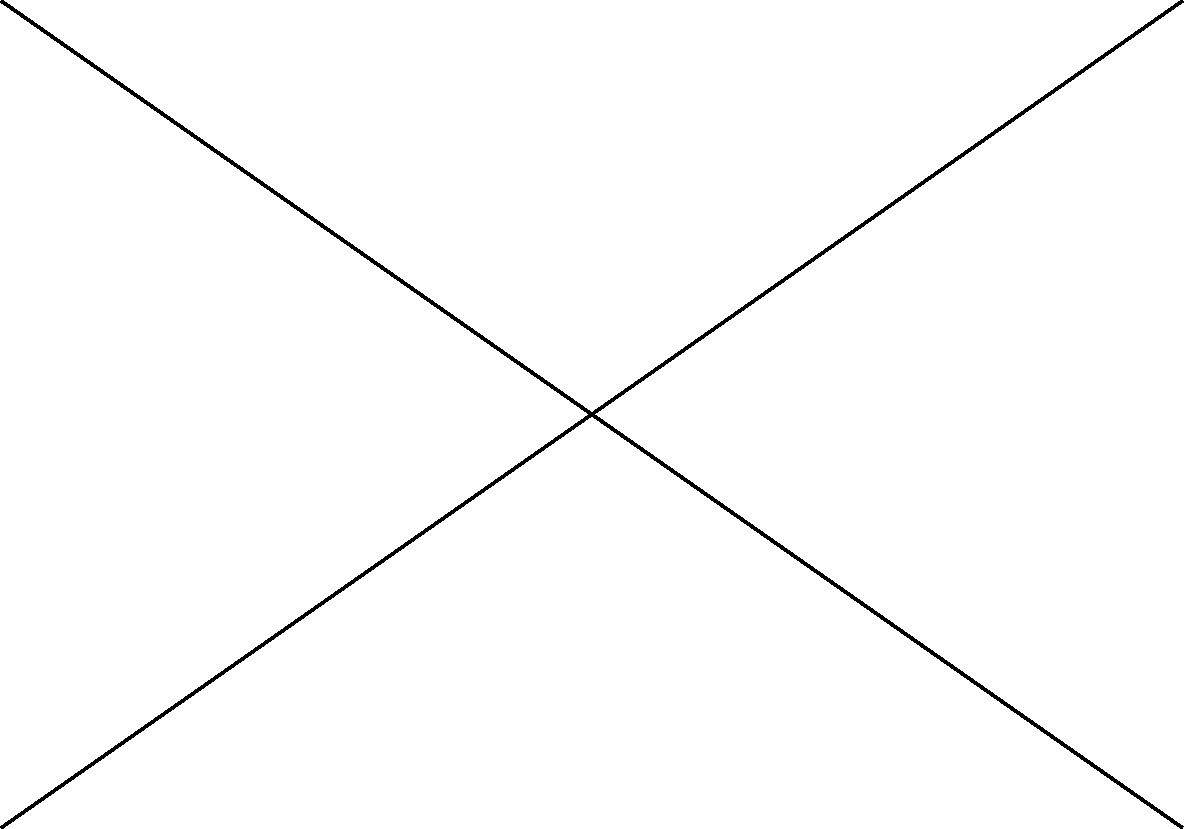
\includegraphics[width=.65\linewidth]{placeholder}
  \caption[An illustration of the N--dimensional parametrisation of a shape
  difference between two datasets.]{Illustration of the calculation of a ratio
    of probability densities in a single dimension.}
  \label{fig:1d-rw-illustration}
\end{figure}

\subsection{$N$-dimensional Parametrisation}
\label{sec:ND-reweight}

As already alluded to in the previous section there are issues with the
parametrisation in a single dimension. Not only is the mapping only guaranteed
to work in a single dimension but if the technique is applied sequentially on
one variable after another the mapping from the first step can be undone by the
second. That is to say that if one calculates the ratio~\ref{eq:1D-ratio} with
$i=1$ and $i=2$ the re-weighting by $r(x_2)$ will not preserve the agreement
between the two predictions that would be achieved by the re-weighting with
$r(x_1)$. It is clear that this is because a ratio for a given $x_i$ only encode
information relating to the PDFs $p(x_i|\theta_0)$ and $p(x_i|\theta_1)$ whereas
what is wanted is something that encodes the multi-variate distributions
$p(\vec{x}|\theta_0)$ and $p(\vec{x}|\theta_1)$.

A function capable of providing compression of the full multi-variate
distribution has already been discussed, these are the functions that one
obtains when training a machine learning algorithm such as those mentioned
in chapter~\ref{ch:ml}. Functions of the form given in
equation~\ref{eq:ml-general} can encode information from the multi-variate
input $\vec{x}$ into a lower dimensional $\vec{y}$ that captures the
correlations between the different elements of the inputs $\vec{x}$.
Specifically for this parametrisation the model is trained to classify events as
coming from either the Monte-Carlo generator with parameters $\theta_0$ or
$\theta_1$, the output is therefore written as $\vec{y} = [y_0, y_1]$ where each
term in the vector represents the probability that an event comes from
$p(\vec{x} | \theta_0)$ or $p(\vec{x} | \theta_1)$ respectively. Note that the
choice of output function in the model ensure that probability is conserved,
i.e. $y_0 + y_1 = 1$. This technique has been demonstrated in the
literature~\cite{cranmer2016approximating} where the mathematical details are
discussed in more detail.

Our setup allows to create the following approximation
\begin{equation}
  r(\vec{x}) =  \frac{p(\vec{x}|\vec{\theta}_{1})}{p(\vec{x}|\vec{\theta}_{0})}
  \approx \frac{F(\vec{x}, \vec{w})[1]}{F(\vec{x}, \vec{w})[0]},
  \label{eq:bdtr-approximation}
\end{equation}
where $F$ is our trained model whose hyper-parameters we can considered fixed
and drop from the notation (previously denoted $\vec{\theta}$ in
chapter~\ref{ch:ml}). The numbers in the square brackets indicate which element
of the $\vec{y}$ is being selected. Once the above approximation is made the
steps to generate weights and perform a parameterisation of the difference in
shape between two predictions is the same as in the one dimensional case. By
placing certain restrictions on $F$ one can turn the approximation into an
equivalence, this is discussed in~\cite{VHModellingNote2019}, however for what
is considered here the approximation will be the focus.
Figure~\ref{fig:nd-rw-illustration} shows an illustration of the
$N$--dimensional parametrisation procedure.
\begin{figure}[t]
  \centering
  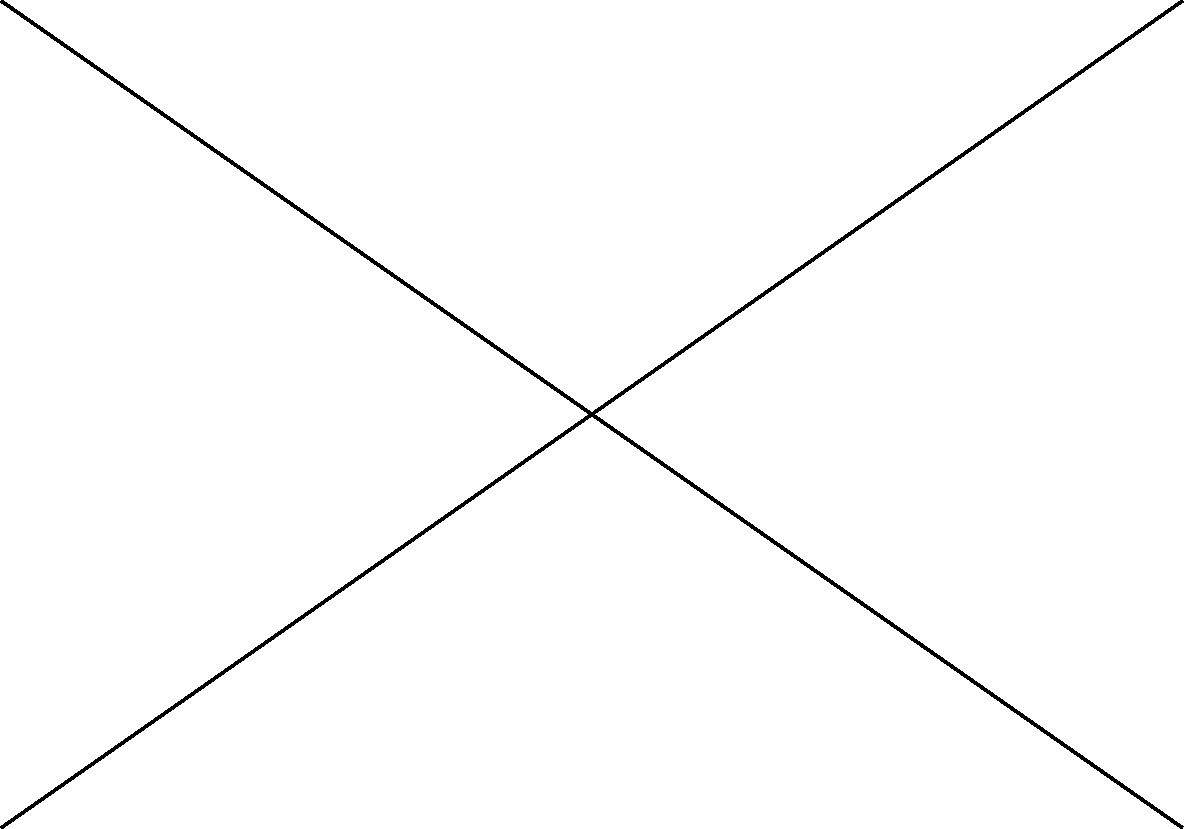
\includegraphics[width=.65\linewidth]{placeholder}
  \caption{Illustration of the calculation of a ratio of probability densities
    using a trained classifier $F$ as a means to compress the multi-variate
    distributions into a single variate one.}
  \label{fig:nd-rw-illustration}
\end{figure}
This parametrisation will be referred to in the analysis as the BDTr method
short for BDT re-weighting as the choice of classifier is a BDT.

\subsection{Hybrid $\mathbf{(N - 1)}$--Dimensional Parametrisation}
\label{sec:hybrid-reweight}

It is possible to combine the aforementioned parametrisation strategies into a
single strategy. This is achieved by first re-weighting using the 1--dimensional
technique and then training the classifier on the re-weighted distributions and
proceeding with the $N$--dimensional parametrisation as usual. In principle the
1--dimensional re-weighting can be performed a number of times sequentially
before training the classifier and so therefore a general $(N-k)$--dimensional
strategy can be formed, however in this analysis the 1--dimensional re-weighting
is only applied once before training.

The hybrid approach yields two parametrisations one that parametrising the
difference between the two samples in the single variable used in the
1--dimensional re-weighting and a second that parametrises the remaining
variables using the density ratio formed by using the classifier trained on the
re-weighted distributions. This approach will be referred to as the factorised
BDTr method as the single variable that is not included in the classifier that
is used to generate the multi-dimensional parametrisation is considered to be
factored out.

There are a number of reasons why one might want to factor out a single variable
from the multi-dimensional procedure that naively looks superior in every way to
the 1--dimensional approach. One must considered that when comparing two
Monte-Carlo based generators internal parameters may be used in one of those
generators that are not used in other, this is one reason why a smooth
interpolation between generators may not actually exist. Given that the
parametrisation generated by any of these methods will be input into a
profile-likelihood fit as a Gaussian constrained nuisance parameter that is
varied in a smooth and continuous manner there is therefore incongruity between
the nature of the nuisance parameter and the underlying mapping between
generators. A second nuisance parameter arising from the factorised variable
therefore at least allows the profile-likelihood fit to control more precisely
the histograms relating to that variable. The choice of factorised variable is
also relevant to the choice of using the hybrid method, for example in the fit
the histograms entering in the control regions are of $P_T^V$ and so it may be
sensible to give the fit a parameter to directly control the shape of this
variable.

\section{Experimental Systematic Uncertainties}
\label{sec:experimental-systs}

This section describes experimental systematic uncertainties, these arise due to
limitations of the hardware discussed in chapter~\ref{ch:detector} and
reconstruction algorithms described in chapter~\ref{ch:recon}. All of these
uncertainties are provided by different combined performance (CP) groups and
made centrally available to members of the ATLAS collaboration, this ensures a
consistent understanding of the performance of the detector and centrally
provided reconstruction algorithms in Athena. A summary of all of the
experimental systematic uncertainties used in the analysis can be found in
table~\ref{tab:expSyst}.
\begin{longtabu}{XX}
  \caption[A summary of experimental systematic uncertainties.]{A summary of the
    experimental systematic uncertainties considered in the analysis. They are
    listed by the name of the nuisance parameter entering into the
    profile-likelihood fit and a short description is provided of each
    uncertainty.}
  \label{tab:expSyst}\\
  \toprule
  {\bfseries Systematic uncertainty} & {\bfseries Short description} \\
  \midrule
  \endfirsthead
  \toprule
  {\bfseries Systematic uncertainty} & {\bfseries Short description} \\
  \midrule
  \endhead
  \midrule
  \multicolumn{2}{c}{Continued}\\   \bottomrule
  \endfoot
  \bottomrule
  \endlastfoot
  {\bfseries Event} & \\
  Luminosity & uncertainty on total integrated luminosity \\
  Pileup Re-weighting & uncertainty on pileup re-weighting \\
  {\bfseries Triggers} & \\
  \texttt{EL\_EFF\_Trigger\_Total\_1NPCOR\_PLUS\_UNCOR} &  electron trigger efficiency uncertainty\\
  \texttt{MUON\_EFF\_TrigStatUncertainty} &  \multirow{2}{*}{muon trigger efficiency uncertainty} \\
  \texttt{MUON\_EFF\_TrigSystUncertainty} & \\
  \texttt{METTrigStat}  &  \multirow{2}{*}{$E_{\mathrm{T}}^{\text{miss}}$trigger efficiency uncertainty} \\
  \texttt{METTrigTop/Z} & \\
  \texttt{METTrigSumpt} & \\
  {\bfseries Electrons}&\\%&\\
  \texttt{EL\_EFF\_Reco\_Total\_1NPCOR\_PLUS\_UNCOR} &  reconstruction efficiency uncertainty \\
  \texttt{EL\_EFF\_ID\_Total\_1NPCOR\_PLUS\_UNCOR} &  ID efficiency uncertainty \\
  \texttt{EL\_EFF\_Iso\_Total\_1NPCOR\_PLUS\_UNCOR} &  isolation efficiency uncertainty \\
  \texttt{EG\_SCALE\_ALL} &        energy scale uncertainty \\
  \texttt{EG\_RESOLUTION\_ALL} &    energy resolution uncertainty \\
  {\bfseries Muons}&\\
  \texttt{MUON\_EFF\_RECO\_STAT} &  \multirow{2}{*}{reconstruction and ID efficiency uncertainty for muons with $p_{\mathrm{T}}$\ $>$ 15 \GeV} \\
  \texttt{MUON\_EFF\_RECO\_SYS} &  \\
  \texttt{MUON\_EFF\_RECO\_STAT\_LOWPT} & \multirow{2}{*}{reconstruction and ID efficiency uncertainty for muons with $p_{\mathrm{T}}$\ $<$ 15 \GeV} \\
  \texttt{MUON\_EFF\_RECO\_SYS\_LOWPT} &  \\
  \texttt{MUON\_EFF\_TTVA\_STAT} &  \multirow{2}{*}{track-to-vertex association efficiency uncertainty} \\
  \texttt{MUON\_EFF\_TTVA\_SYS} &                      \\
  \texttt{MUON\_ISO\_STAT} &  \multirow{2}{*}{isolation efficiency uncertainty} \\
  \texttt{MUON\_ISO\_SYS} &                     \\
  \texttt{MUON\_ID} & momentum resolution uncertainty from inner detector        \\
  \texttt{MUON\_MS} &  momentum resolution uncertainty from muon system        \\
  \texttt{MUON\_SCALE} &   momentum scale uncertainty         \\
  \texttt{MUON\_SAGITTA\_RHO} & \multirow{2}{*}{charge dependent momentum scale uncertainty} \\
  \texttt{MUON\_SAGITTA\_RESBIAS} &  \\
  {\bfseries Jets and $\bm{b}$-tagging}&\\
  \texttt{JET\_CR\_JET\_EffectiveNP\_Detector1,2} & energy scale uncertainty from the in situ analyses (detector) \\
  \texttt{JET\_CR\_JET\_EffectiveNP\_Modelling1,...,4} & energy scale uncertainty from the in situ analyses (modelling) \\
  \texttt{JET\_CR\_JET\_EffectiveNP\_Statistical1,...,6} & energy scale uncertainty from the in situ analyses (stat) \\
  \texttt{JET\_CR\_JET\_EffectiveNP\_Mixed1,2,3} & energy scale uncertainty from the in situ analyses (mixed terms) \\
  \texttt{JET\_CR\_JET\_EtaIntercalibration\_Modeling} & energy scale uncertainty on eta-intercalibration (modelling)\\
  \texttt{JET\_CR\_JET\_EtaIntercalibration\_TotalStat} & energy scale uncertainty on eta-intercalibrations (statistics/method) \\
  \texttt{JET\_CR\_JET\_EtaIntercalibration\_NonClosure\_highE} & \multirow{3}{*}{energy scale uncertainty on eta-intercalibrations (non-closure)} \\
  \texttt{JET\_CR\_JET\_EtaIntercalibration\_NonClosure\_negEta} &\\
  \texttt{JET\_CR\_JET\_EtaIntercalibration\_NonClosure\_posEta} &\\
  \texttt{JET\_CR\_JET\_BJES\_Response} &  \\
  \texttt{JET\_CR\_JET\_Flavor\_Composition} & energy scale uncertainty on $V\!V$ and \VH\ sample's flavour composition \\
  & {$\rightarrow$ Independent NP for : "\texttt{\_Top}", "\texttt{\_Vjets}", "\texttt{\_VV}" processes } \\
  \texttt{JET\_CR\_JET\_Flavor\_Response} & energy scale uncertainty on samples' flavor response \\
  \texttt{JET\_CR\_JET\_Pileup\_OffsetMu} & energy scale uncertainty on pile-up (Mu dependent) \\
  \texttt{JET\_CR\_JET\_Pileup\_OffsetNPV} & energy scale uncertainty on pile-up (NPV dependent) \\
  \texttt{JET\_CR\_JET\_Pileup\_PtTerm} & energy scale uncertainty on pile-up (pt term) \\
  \texttt{JET\_CR\_JET\_Pileup\_RhoTopology} & energy scale uncertainty on pile-up (density $\rho$) \\
  \texttt{JET\_CR\_JET\_PunchThrough\_MC16} & energy scale uncertainty for punch-through jets \\
  \texttt{JET\_CR\_JET\_SingleParticle\_HighPt} & energy scale uncertainty from the behavior of high-pT jets \\
  \texttt{JET\_CR\_JET\_JER\_EffectivNP\_1,...6,7restTerm} & energy resolution uncertainty split into 7 components \\
  \texttt{JET\_CR\_JET\_JER\_DataVsMC} & energy resolution additional uncertainty difference between data than MC resolutions \\
  \texttt{JET\_JvtEfficiency} & JVT efficiency uncertainty \\
  \texttt{FT\_EFF\_Eigen\_B0,...,45} & \multirow{3}{*}{\parbox{11cm}{$b$-tagging efficiency uncertainties (``BTAG\_LOOSE'') in continuous mode: 45 components for $b$ jets, 20 for $c$ jets and 20 for light jets}} \\
  \texttt{FT\_EFF\_Eigen\_C0,...,20} &\\
  \texttt{FT\_EFF\_Eigen\_L0,...,20} &\\
  \texttt{FT\_EFF\_Eigen\_extrapolation} & $b$-tagging efficiency uncertainty on the extrapolation to high-$p_{\mathrm{T}}$\ jets \\
  \texttt{FT\_EFF\_Eigen\_extrapolation\_from\_charm} & $b$-tagging efficiency uncertainty on tau jets \\
  {\bfseries $\bm{E}_{\mathrm{T}}^{\text{miss}}$}&\\
  \texttt{MET\_SoftTrk\_ResoPara} & track-based soft term related longitudinal resolution uncertainty \\
  \texttt{MET\_SoftTrk\_ResoPerp} &  track-based soft term related transverse resolution uncertainty \\
  \texttt{MET\_SoftTrk\_Scale} & track-based soft term related longitudinal scale uncertainty \\
  \texttt{MET\_JetTrk\_Scale} & track MET scale uncertainty due to tracks in jets \\
  {\bfseries Taus}&\\
  \texttt{TAUS\_TRUEHADTAU\_SME\_TES\_DETECTOR} & energy scale uncertainty: single-particle response + threshold \\
  \texttt{TAUS\_TRUEHADTAU\_SME\_TES\_INSITU} & energy scale uncertainty: total from in-situ measurement \\
  \texttt{TAUS\_TRUEHADTAU\_SME\_TES\_MODEL} & energy scale uncertainty: modelling + closure \\
  \bottomrule
\end{longtable}

\subsection{Luminosity and Pile-up}
\label{sec:lumisys}

As discussed in chapter~\ref{ch:detector} luminosity is used to measure how much
data is recorded by the detector in any span of time. The uncertainty is
calculated for each year of running and is determined to be  2.1\%, 2.6\%,
2.4\%, and 2.0\% for the years 2015, 2016, 2017, 2018 respectively. A combined
uncertainty is calculated for the entire period 2015--2018 at 1.7\%. The
methodology used to calculate this figure is similar to that detailed
in~\cite{lumiDetermine}, from calibrations of the luminosity scale using x--y
beam-separation scans~\cite{lumiTwiki}.

Pile-up uncertainties are computed by changing the nominal data scale of
$1.0/1.03$ to $1.0/1.00$ and $1.0/1.18$ to get the up and down variations
respectively~\cite{puTWiki}.

\subsection{Triggers}
\label{sec:trigsys}

\subsubsection{\texorpdfstring{$E_T^{\text{miss}}$}{MET} Triggers}

Scale factors are derived for the $E_T^{\text{miss}}$ triggers using
$W(\mu,\nu)$ + jets events as outlined in~\cite{VHObjectNote2019}.

Three uncertainties are taken into account, the statistical error on the dataset
used to derived the scale factor \texttt{METTrigStat}, a parameter used to
account for the choice of physics process and the effect that might have on the
determination of the scale factor \texttt{METTrigTop} and \texttt{METTrigSumPt}
which aims to account for dependence of the offline $S_T$ (as defined
in~\ref{sec:0lep-selection}) on the trigger efficiency. The uncertainty
\texttt{METTrigTop} is named as such because it is derived from a comparison of
the scale factors as calculated with a $t\bar{t}$ sample and compared to the
nominal sample. The uncertainty relating to $S_T$ is only applied to events
recorded in 2017 due to a specific trigger used in this year.

\subsubsection{Lepton trigger}

The CP group recommendations for the lepton triggers can be found
in~\cite{VHObjectNote2019}. The group provide a tool for determining the lepton
trigger systematic error which is implemented in the CxAOD Framework (mentioned
in section~\ref{sec:cxaod}). The nuisance parameter
\texttt{EL\_EFF\_Trigger\_Total\_1NPCOR\_PLUS\_UNCOR} is used to control the overall
uncertainty on the electron trigger. For the muons, the tool returns two components
\texttt{MUON\_EFF\_TrigSystUncertainty} and \texttt{MUON\_EFF\_TrigStatUncertainty}
which account for the systematic error and the statistical error on scale factor
respectively. An up and down variation of 1-$\sigma$ are used for all of the
aforementioned nuisance parameters.

\subsection{Electrons}

\subsubsection{Electron Efficiency Uncertainties}

The efficiency of the electron reconstruction and identification (discussed
in~\ref{subsec:electrons}) has a systematic uncertainty provided by the relevant
CP group called \texttt{ElectronEfficiencyCorrection}~\cite{electronTWiki}.
These have been calculated using the full run 2 data. Reconstruction is 97-99\%
efficient across the full $p_T$~spectrum. Identification has an efficiency scale
factor is available from $p_T>7$~\GeV. An isolation efficiency scale factor is
also included. The latest uncertainties that are available include scale factors
for $p_T>150$~\GeV\ that are unity due to the available sample being to small in
statistics to measure a scale factor~\footnote{Check if this is for all electron
  systs}. An additional systematic uncertainty of $\pm 2\%$ is assigned above
150~\GeV\ to over this shortcoming. The above uncertainties are controlled by
\texttt{EL\_EFF\_ID\_Total\_1NPCOR\_PLUS\_UNCOR},
\texttt{EL\_EFF\_Reco\_Total\_1NPCOR\_PLUS\_UNCOR}, and
\texttt{EL\_EFF\_Iso\_Total\_1NPCOR\_PLUS\_UNCOR} in the profile-likelihood fit.

\subsubsection{Electron Energy Scale and Resolution Uncertainties}

Energy scale and resolution systematic uncertainties have been provided by the
relevant CP group~\cite{EgammaCalibTWiki}. Whilst there are a large number of
uncertainties provided by the group, this analysis is not very sensitive to the
energy scale or resolution of electrons and therefore only two uncertainties are
considered which are called \texttt{EG\_RESOLUTION\_ALL} and
\texttt{EG\_SCALE\_ALL}.

\subsection{Muons}

\subsubsection{Muon Efficiency Systematic Uncertainties}

Samples of $Z \to \mu\mu$ and $J/\psi \to \mu\mu$ events from the full 2015
dataset (corresponding to 3.2~fb$^{-1}$) are used to calculate scale factors to
account for uncertainties in the reconstruction, isolation and track-to-vertex
association~\cite{muonTWiki}. These scale factors are valid in the full $p_T$
spectrum with the $J/psi$ measurement providing more accurate determination in
the $p_T$<15~\GeV\ region and the Z measurement being more accurate in the
$p_T$>15~\GeV\ region. Four independent systematic uncertainties are considered
which are called \texttt{MUON\_EFF\_RECO\_STAT},

\texttt{MUON\_EFF\_RECO\_STAT\_LOWPT}, \texttt{MUON\_EFF\_RECO\_SYS},
\texttt{MUON\_EFF\_RECO\_SYS\_LOWPT}, which are split based on whether or not
they come from the high or low $p_T$ measurement. Statistical and systematic
uncertainties to the isolation scale factor are controlled by
\texttt{MUON\_EFF\_ISO\_STAT} and \texttt{MUON\_EFF\_ISO\_SYS} respectively.
They are supported in the range of $10 < p_T < 500$~\GeV. For muons outside of
this range, a scale factor of 1$\pm$0.05 is used.
\texttt{MUON\_EFF\_TTVA\_STAT} and \texttt{MUON\_EFF\_TTVA\_SYS} control the
systematic uncertainty on the scale factor of the cuts on the impact parameter
significance and the $|z_0\sin\theta|$ which estimate the error on
track-to-vertex association. All of the above systematic uncertainties are
derived using $\pm 1\sigma$ variations in the relevant samples.

\subsubsection{Muon Momentum Scale and Resolution Uncertainties}

Similarly to the electron energy scale and resolution uncertainties described
above the muon momentum scale and resolution uncertainties are provided by the
relevant CP group~\cite{muonTWiki}. Measurements of muons have been calibrated
using a sample of  $Z\rightarrow \mu\mu$ events in the region with
$p_T$~>~20~\GeV\ and with a sample of $J/\psi\rightarrow \mu\mu$ events in region
with $p_T$~<~20~\GeV. The nuisance parameters control the uncertainties due to
the inner detector, muon system and the overall momentum scale, they are called
\texttt{MUONS\_ID}, \texttt{MUONS\_MS} and \texttt{MUONS\_SCALE} respectively.
These systematic uncertainties are derived by varying the momentum scale and the
track position in the detector by $\pm 1\sigma$. Two parameters which account
for the charge dependence of the of the momentum scale uncertainty
\texttt{MUON\_SAGITTA\_RHO} and \texttt{MUON\_SAGITTA\_RESBIAS} are also included.

\subsection{Taus}

Taus are not crucial to the analysis and therefore the systematic uncertainties
on the measurement of taus does not have a large effect on the result. The
systematic uncertainties considered in the analysis relating to taus are
\texttt{TAUS\_TRUEHADTAU\_SME\_TES\_DETECTOR},
\texttt{TAUS\_TRUEHADTAU\_SME\_TES\_INSITU} and
\texttt{TAUS\_TRUEHADTAU\_SME\_TES\_MODEL}, which all account for different
sources of energy scale uncertainty.

\subsection{Jets}

As with the other reconstructed objects discussed so far the systematic
uncertainties for jets are provided through a central tool written by the
relevant CP group that is interfaced in the CxAOD Framework. Analyses may choose
between a number of different schemes, the choice for the \VHbb\ analysis is to
use a reduced set of 23 nuisance parameters comi
ng from a reduction using
principal component analysis of the baseline set of parameters. The baseline set
accounts for effects due to eta calibration, high-$p_T$ jets, pile-up, flavour
composition, flavour response, $b$-jets, and punch-through jets. The 23 nuisance
parameters and a short description of each are displayed in
table~\ref{tab:expSyst} under the category jets and $b$-tagging where all of the
relevant nuisance parameters start with \texttt{JET} and
\texttt{JET\_CR\_Flavour\_Composition} represents three independent nuisance
parameters as explained in its short description.

The largest source of uncertainty amongst the chosen set come from the jet
energy scale and the jet energy resolution. The determination of the former is
documented in~\cite{JetCalibration2015} and the latter is determined from data
versus Monte-Carlo prediction comparisons.

\subsection{$E_T^{\text{miss}}$}

Once again $E_T^{\text{miss}}$ systematic uncertainties are implemented via a
centrally available tool written by the relevant CP group and interfaced in the
CxAOD Framework. The tool is configured to account for calorimeter and track
based jets, the uncertainties considered in this analysis are under the heading
$E_T^{\text{miss}}$ in table~\ref{tab:expSyst} and start with \texttt{MET}.

\subsection{Flavour Tagging}

The uncertainties relating to the flavour tagging procedure detailed
in~\ref{sec:btagging} are very important to consider in the analysis as the
tagging itself has a central role in selecting events in all of the leptonic
channels. Each event that has been passed through the tagging algorithms has
event weights that encode the systematic error on the tagging. The following
describes how these scale factors are calculated with reference to the tool
provided by the relevant CP group. For each signal events apply the scale factor
from the CP tool if it has been tagged as a $b$-jet, otherwise apply the
inefficiency scale factor provided by the same tool (which yields the nominal
event weight). For each of the systematic uncertainties considered vary the
scale factor and inefficiency scale factor by the variations provided by the CP
tool and repeat the previous method (note the varied inefficiency scale factor
will no longer yield the nominal event weight). For all histograms that would
enter the profile-likelihood fit a separate histogram is created for each
systematic uncertainty (both an up and down variation where the uncertainties
are two-sided).

Similarly to in the determination of the systematic uncertainties on the jets, a
large number of individual systematics are available (about 40 per jet flavour)
and so in order to have a smaller set to work with a principle component
analysis of the full set is performed by the CP group. For the working point
(70~\%) and reduction scheme chosen in this analysis there are 3 variations for
$b$-jets, 3 variations for $c$-jets and 5 variations for light-jets. These are
named \texttt{FT\_EFF\_Eigen\_Light0}, \texttt{FT\_EFF\_Eigen\_Light1},
\texttt{FT\_EFF\_Eigen\_Light2}, \texttt{FT\_EFF\_Eigen\_Light3},\\
\texttt{FT\_EFF\_Eigen\_Light4}, \texttt{FT\_EFF\_Eigen\_B0},
\texttt{FT\_EFF\_Eigen\_B1}, \texttt{FT\_EFF\_Eigen\_B2},
\texttt{FT\_EFF\_Eigen\_C0}, \texttt{FT\_EFF\_Eigen\_C1} and
\texttt{FT\_EFF\_Eigen\_C2}.

Two additional systematic uncertainties irrespective of reduction scheme are
considered that relate to the $p_T$ extrapolation~\cite{BTaggingExtrap2015} and
charm-to-bottom quark extrapolation, they are called
\texttt{FT\_EFF\_Eigen\_extrapolation}, and
\texttt{FT\_EFF\_Eigen\_extrapolation\_from\_charm} respectively.

\section{Systematic Uncertainties on V + jets Events}
\label{sec:vjets}
Whilst the physics of the W and Z + jets processes leads to them being in
different channels and needing to be treated differently in the analysis, the
underlying theory means that simulation of these processes is coupled,
particularly as they are simulated with the same software.

The V + jets processes are simulated with
\textsc{Sherpa}~2.2.1~\cite{1126-6708-2009-02-007} as mentioned in
section~\ref{sec:composition}, which is interfaced with the
NNPDFs~\cite{Ball:2012cx} for both the matrix element calculation and the parton shower
tuning. Events with many additional jets produced in association with the vector
boson largely contribute to the background in this analysis, therefore a feature
of \textsc{Sherpa}~2.2.1 is used in which it provides a combination of matrix
elements with different parton multiplicities. Up to 2 extra partons are
included in the next-to-leading order matrix element, and 3 or 4 extra partons
are included at leading order in QCD. In order to combine different patron
multiplicities a matching scheme based on the CKKW-L~\cite{Lonnblad:2001iq,
  Lavesson:2005xu} merging technique is used, with a merging scale of $Q_{cut} =
20$~\GeV. Simulation of events with more than 4 extra partons relies on the
parton shower algorithm of \textsc{Sherpa}. The parton shower and underlying
events models are included in \textsc{Sherpa} whose generator adopts a full
5--flavour scheme with b- and c-quarks being treated as massless in the matrix
element, in the version used. Massive quarks can be produced in the parton
shower and heavy flavours (quarks as heavy or heavier than a c-quark) can be
produced directly in the scattering process of the underlying event.

The analysis gains a lot of sensitivity from high $p_T^V$ regions of phase
space, and also has the requirement of two b-tagged jets in the event selection
as mentioned in section~\ref{sec:selection}. It is therefore important to ensure
that a large statistical sample in these regions is available such that
fluctuations are smaller than those that would be found in the data. In order to
achieve this two methods are used, firstly samples are simulated in specific
slices of the larger of the $p_T$ of the vector boson or the $H_T$ of the event.
Events are simulated in the following slices
\begin{equation}
  \text{max}(p_T^V, H_T) = [0\text{--}70, 70\text{--}140, 140\text{--}280, 280\text{--}500, 500\text{--}1000, >1000]~\GeV.
\end{equation}
The dedicated slices at high $\text{max}(p_T^V, H_T)$ ensure a large number of
events are simulated in the high $p_T^V$ region of phase space. Secondly filters
are applied on the flavour of the jets that produced in association with the
vector boson.  The filters used for these samples are shown in
table~\ref{tab:bc-filters}.
\begin{table}[!htb]
  \centering
  \resizebox{0.95\textwidth}{!}{
    \begin{tabular}{lll}
      \toprule
      {\bfseries Filter} & {\bfseries Description} \\
      \midrule
      $b$-filter & at least 1 $b$-hadron with $p_{\mathrm{T}} >$0~GeV and $|\eta|<$4 \\
                         & at least 1 $b$-hadron with $p_{\mathrm{T}} >$5~GeV and $|\eta|<$2.9$^{\dagger}$ \\
      $c$-filter-$b$-veto & at least 1 $c$-hadron with $p_{\mathrm{T}}>$4~GeV and $|\eta|<$3   \\
                         & veto events which pass the $b$-filter  \\
      $c$-veto-$b$-veto & veto events which pass the $b$-filter or the $c$-filter-$b$-veto  \\
      \bottomrule
    \end{tabular}
  }
  \caption{Flavour filters used in the simulation of $V+$jets events. $\dagger$
    this tighter filter is only applied to $Z\to\nu\nu$ samples.}
  \label{tab:bc-filters}
\end{table}
The filters are not applied to the highest slices in $\text{max}(p_T^V, H_T)$.
The filtering strategy for $Z\nu\nu$ samples differs in the mc16e campaign using
a combination of $p_T^Z$ and $m_{jj}$ to better populate the region above the
MET trigger thresholds, and VBF phase spaces with high $m_{jj}$. These samples
also use a tighter b-filter compared to their mc16a/d counterpart which is also
described in table~\ref{tab:bc-filters}. All nominal V + jets samples with the
corresponding max($H_T$,$p_T^V$) slices and flavour filters are listed in
tables~\ref{tabular:mc_samples_Wjets} \ref{tabular:mc_samples_Zlljets}, and
\ref{tabular:mc_samples_Zvvjets} in the appendices.
+
A set of alternative predictions are used for a number of purposes in the
analysis, one such purpose is to investigate any discrepancies that may arise
between data and the nominal prediction. If the same discrepancy is present when
comparing he alternative prediction to data then the discrepancy may arise from
experimental error rather than weaknesses in the modelling. One kind of
modelling uncertainty also relies on the comparison of two predictions, for
example the nominal versus the alternative.

The alternative samples are generated using
\textsc{MadGraph}~5~\cite{MADGRAPH5_aMC@NLO} interfaced to \textsc{Pythia}~8 for
the modelling of the parton shower and the underlying event. The
\textsc{MadGraph}~5 v2 generator provides a LO (QCD) description of these
processes, merging together matrix-element calculations with different parton
multiplicities, up to 4 additional jets, higher jet multiplicities are modelled
by the parton shower algorithm. The merging scheme applied to combine different
parton multiplicities is the same as for the nominal samples, the CKKW-L scheme,
but has a merging scale of $Q_{cut} = 30$~\GeV. For the LO ME calculation the
NNPDF2.3 LO PDFs are used, with $\alpha_S = 1.3$.  Similarly to
\textsc{Sherpa}~2.2.1, also \textsc{MadGraph}~adopts a full 5-flavour scheme
with massless quarks in the ME calculation, while massive quarks can be produced
by the parton shower. All alternative V + jets samples are listed in
tables~\ref{tabular:zjetsAlternativeSamples} and
\ref{tabular:wjetsAlternativeSamples} in the appendices.

As well as using an alternative Monte-Carlo generator the nominal generator,
\textsc{Sherpa}, includes systematic variations internally. Every
\textsc{Sherpa}~2.2.1 V + jets sample has an event weight corresponding to each
of the variations detailed in table~\ref{tab:sherpa-variations}\footnote{Some of
the variations cannot be produced by \textsc{Sherpa}~2.2.1 and so
\textsc{Sherpa}~2.1 is used instead. For these variations half of the variation
in each direction is taken as the uncertainty rather than comparing to the
central value of the \textsc{Sherpa}~2.2.1 prediction.}.
\begin{table}
  \centering
  \begin{tabular}{ l l l }
    \toprule
    \bfseries{Variation} & \multicolumn{2}{l}{\bfseries{Values}} \\
    \midrule
    \multicolumn{3}{l}{\bfseries{Sherpa 2.2.1}} \\
    Factorisation scale ($\mu_F$) & $2\mu_F$ & 0.5$\mu_F$ \\
    Renormalisation scale ($\mu_R$) & $2\mu_R$ & 0.5$\mu_R$ \\
    PDF Variation & MMHT2014nnlo68cl & CT14nnlo \\
    &&\\
    \multicolumn{3}{l}{\bfseries{Sherpa 2.1}} \\
    Re-summation scale ($\mu_S$) & $2\mu_S$ & 0.5$\mu_S$ \\
    CKKW Merging scale & 15 \GeV & 30 \GeV \\
    \bottomrule
  \end{tabular}
  \caption{A summary of the Sherpa 2.2.1 and Sherpa 2.1 internal variations that
  are used to model V + jets processes.}
  \label{tab:sherpa-variations}
\end{table}

\subsubsection{V + jets Cross Section}
The V + jets cross sections are known at NNLO (QCD)~\cite{Butterworth:1287902},
the higher order cross sections are used to normalise the V+jets samples in the
analysis. For the W + jets samples the total cross section from \textsc{Sherpa} or
from \textsc{MadGraph}, averaged across all 3 lepton flavours taking into account the
different hadron filter efficiencies, is scaled to the NNLO prediction obtaining
scaling factor of $k_{\text{NNLO}}^{\text{QCD}} = 0.9702$.

For Z + jets some subtleties must be considered. For $Z \to \ell\ell$ + jets the
cut at generator level, $m_{\ell\ell}>40$ \GeV, must be taken into account. The
NNLO calculation uses a cut of $66<m_{\ell\ell}<116$ \GeV, which can be applied
at truth level to the samples of this analysis in order to get the scaling
correct as follows:
\begin{equation}
  k_{\text{NNLO}}^{\text{QCD}} = \frac{\sigma_{\text{NNLO}}(66<m_{\ell\ell}<116\,{\GeV})}{\sigma_{\textsc{Sherpa},\textsc{MadGraph}}(66<m_{\ell\ell}<116\,{\GeV})},
  \label{eq:nnlo-vjets-k}
\end{equation}
hence the scaling factor is found to be $0.9751$. For $Z \to \nu\nu$ +jets the
NNLO no theoretical cross section is available. Values from the
Particle Data Group (PDG)~\cite{PDG} are used to correct for the difference
between the BR($Z \to \nu\nu$) and BR($Z \to \ell\ell$), and the NNLO cross
section is used without any mass cuts and with the $Z/\gamma^*$ interference
removed. The scaling factor is therefore calculated to be $0.9728$. It is not
necessarily expected that the scaling factors should be different for $Z \to
\ell \ell$ and $Z \to \nu \nu$ events but this can be explained as both
\textsc{Sherpa} and \textsc{MadGraph} used different branching ratios for these
two processes in their generators compared with those used by the higher order
theoretical calculations.

\subsection{Systematic Uncertainties on W + jets Events}
A number of nuisance parameters are introduced to account for modelling
uncertainties on the W + jets background process. These uncertainties are
considered and derived in the 0-- and 1-- lepton channels only as the amount of
W + jets background present in the 2--lepton channel is negligible. A summary of
all of the uncertainties for this background can be found in
table~\ref{tab:wjets_systematics}.

The nominal and alternative predictions described in~\ref{sec:vjets} are used to
in the determination of all of the values described in the following. 

\subsubsection{Normalisation and Acceptance Uncertainties}

A summary of the normalisation uncertainties is shown in
table~\ref{tab:wjetsnorm}.
\begin{table}[!htb]
  \centering
  \resizebox{\textwidth}{!}{
    \begin{tabular}{llS[table-format=3.2]S[table-format=3.2]S[table-format=3.2]S[table-format=3.2]S[table-format=3.2]S[table-format=3.2]}
      \toprule
      &  & \multicolumn{3}{c}{\bfseries 2--jet} & \multicolumn{3}{ c }{\bfseries 3--jets} \\
      {\bfseries Name} & {\bfseries Process} & {\bfseries CR$_{\text{low}}$} & {\bfseries SR} & {\bfseries CR$_{\text{high}}$} &  {\bfseries CR$_{\text{low}}$} & {\bfseries SR} & {\bfseries CR$_{\text{high}}$} \\
      \midrule
      {\bfseries 0-Lepton} & & & & & & & \\
      {\texttt{SysWbbNorm\_L0}}    & W+hf   &  5\% &  5\% & N/A  &  N/A & N/A & N/A    \\
      {\texttt{SysWbbCRSRextrap}}        & W+hf   &   -7.7\% &  N/A & 14.9\%  &  -5.6\% & N/A & 7.0\%    \\
      {\bfseries 1-Lepton} & & & & & & & \\
      {\texttt{SysWclNorm}}             & W+l    &   \multicolumn{6}{ c }{   32\% } \\
      {\texttt{SysWlNorm}}              & W+cl   &   \multicolumn{6}{ c }{  37\%  }\\
      {\texttt{norm\_Wbb\_J2}}           & W+hf   &   \multicolumn{3}{ c }{ Floating Normalisation} & N/A & N/A & N/A \\
      {\texttt{norm\_Wbb\_J3}}           & W+hf   &  N/A & N/A & N/A & \multicolumn{3}{ c }{ Floating Normalisation} \\
      {\texttt{SysWbbCRSRextrap}}        & W+hf   &   -11.5\% &  N/A & 14.8\%  &  -3.6\% & N/A & 5.1\%    \\
      \bottomrule
    \end{tabular}
  }
  \caption[$W+$jets normalisation and acceptance uncertainties.]{A summary of the
    nuisance parameters used to account for the uncertainty on the normalisation
    of simulated $W+$jets predictions. The values shown correspond to a prior
    representing a 1--$\sigma$ shift in the relevant Gaussian penalty term.}
  \label{tab:wjetsnorm}
\end{table}
A single nuisance parameter is introduced for each of the W + cl and W + l
processes which are both heavily suppressed by the analysis requirement of two
b-tagged jets. There is a large mismodelling of the normalisation of the W + hf
process and so floating normalisations are used separately in the 2--jet and
3--jet categories. Priors for several acceptance uncertainties are calculated using
equation~\ref{eq:acceptance-dr}\footnote{Whilst the priors are obtained with the
  double ratio formula involving two regions, the effect of the uncertainty is
  applied to only one of the two regions. This does not affect the result but
  only the interpretation of the resulting acceptance factor.} which are used to
control the migration of events between the 0-- and 1--lepton channels and the
migration between the $\Delta R(b, \bar{b})$ regions.

The parameter controlling migration between the two leptonic channels
\texttt{SysWbbNorm\_L0} is applied to both the 2--jet and 3--jet regions of the
0--lepton channel. The choice to apply to the 0--lepton channel and not the
1--lepton channel is made because the 1--lepton channel provides a better
constraint on the W + hf process. Whilst all alternative predictions are
considered the size of this prior is dominated by the difference between the
nominal prediction and \textsc{MadGraph}.

Migration between the $\Delta R(b, \bar{b})$ control regions and the signal
region is controlled by one parameter per control region. Named
\texttt{SysWbbCRSRextrap} it can be seen in table~\ref{tab:wjetsnorm} that it is
applied in each of the control regions, it is also correlated across jet
multiplicity and leptonic channel. The shape uncertainty which uses the BDTr
method discussed in section~\ref{sec:ND-reweight} induces migration effects
across the analysis regions, however in order to increase the degrees of freedom
available to the profile-likelihood fit that systematic is taken as a shape only
effect. The migrations induced by the shape uncertainty agree well with those
derived from comparisons between nominal and alternative predictions, and the
sign of the final priors is determined by migration due to the shape
uncertainty. The magnitude of the prior is calculated as the quadrature sum of
the difference between the nominal prediction and \textsc{MadGraph} as well as
the scale and parton density function variations included in \textsc{Sherpa}.
There is no dedicated nuisance parameter to control the migration between the
$p_T^V$ regions of the analysis as this migration is controlled by the $p_T^V$
shape uncertainty.

\subsubsection{Flavour Composition Uncertainties}

As introduced at the start of this chapter the W + jets background has a W + hf
component that is comprised of the $bb$, $bc$, $bl$ and $cc$ sub-components. The
fractional contribution of each of these sub-components is detailed in
table~\ref{tab:whf-comp}.
\begin{table}[h]
  \centering
  \begin{tabular}{lS[table-format=3.2]S[table-format=3.2]S[table-format=3.2]S[table-format=3.2]S[table-format=3.2]S[table-format=3.2]}
    \toprule
    & \multicolumn{3}{c}{\bfseries 2 jet}  &  \multicolumn{3}{c}{\bfseries 3 jet} \\
    {\bfseries Process} & {\bfseries CRLow} & {\bfseries CRHigh} & {\bfseries SR} & {\bfseries CRLow} & {\bfseries CRHigh} & {\bfseries SR} \\
    \midrule
    {\bfseries 0-lepton} & & & & & & \\
    $Wcc$ & 0.03 & 0.02 & 0.03 & 0.03 & 0.03 & 0.04\\
    $Wbl$ & 0.01 & 0.03 & 0.09 & 0.01 & 0.02 & 0.07\\
    $Wbc$ & 0.02 & 0.05 & 0.10 & 0.02 & 0.04 & 0.10\\
    $Wbb$ & 0.94 & 0.90 & 0.78 & 0.94 & 0.91 & 0.79\\
    {\bfseries 1-lepton} & & & & & & \\
    $Wcc$ & 0.03 & 0.05 & 0.03 & 0.03 & 0.04 & 0.03\\
    $Wbl$ & 0.01 & 0.03 & 0.01 & 0.01 & 0.05 & 0.02\\
    $Wbc$ & 0.03 & 0.15 & 0.07 & 0.03 & 0.13 & 0.05\\
    $Wbb$ & 0.93 & 0.77 & 0.89 & 0.94 & 0.77 & 0.90\\
    \bottomrule
  \end{tabular}
  \caption[A breakdown of flavour subprocesses making up the W + heavy flavour
  process.]{The contribution of each $W$+hf subprocesses to the total $W$+hf
    yields in all 1-lepton and 0-lepton channels analysis regions expressed as a
    decimal.}
  \label{tab:whf-comp}
\end{table}
Flavour composition uncertainties are computed using
equation~\ref{eq:acceptance-dr} for each sub-component, the calculated priors
are summarised in tables~\ref{tab:wjets-flavour-comp} separately in the 0-- and
1--lepton channels~\footnote{Whilst these numbers were calculated using the
  categorisation and samples of this analysis, due to incomplete availability of
  \textsc{Sherpa} internal variations a set of numbers calculated in a previous
  iteration of the analysis are displayed and used.}.
\begin{table}[!htbp]
  \centering
  \begin{tabular}{llll}
    \toprule
    {\bfseries Name} & {\bfseries Ratio} & {\bfseries Prior} & {\bfseries Region}\\ 
    \midrule
    \multirow{ 2}{*}{\texttt{SysWbcWbbRatio}}  & \multirow{ 2}{*}{$W$+bc/$W$+bb} & 15\% & 0-Lepton \\
             &    & 30\% & 1-Lepton \\
    \multirow{ 2}{*}{\texttt{SysWblWbbRatio}}  & \multirow{ 2}{*}{$W$+bl/$W$+bb} &  10\% & 0-Lepton \\
             &    & 30\% & 1-Lepton \\
    \multirow{ 2}{*}{\texttt{SysWccWbbRatio}} & \multirow{ 2}{*}{$W$+cc/$W$+bb} &  26\% & 0-Lepton\\
             &    &  23\% & 1-Lepton\\
    \bottomrule
  \end{tabular}
  \caption{A summary of the flavour composition uncertainties applied to the
    components of the W + hf process. All uncertainties are only applied to
    events belonging to the component in the numerator of the ratio in the
    region specified.}
  \label{tab:wjets-flavour-comp}
\end{table}
The flavour composition uncertainties are dominated by the difference between
\textsc{Sherpa} and \textsc{MadGraph}. Individual uncertainties for different
jet multiplicities or analysis regions are not considered necessary due to a
small amount of non-$bb$ events remaining after the 2 b-tag requirement is
imposed.

\subsubsection{Shape Uncertainties}

The hybrid $(N-1)$--dimensional parametrisation technique described
in~\ref{sec:hybrid-reweight} is used to generate uncertainties on the shape of
the distributions of the W + jets background. The variable that has been
factorised out is $p_T^V$ and so there are nuisance parameters which control the
$p_T^V$ shape in each of the 2-- and 3--jet categories as well as a nuisance
parameter that controls the multi-variate shape uncertainty across all regions
and jet multiplicities. These nuisance parameters are summarised in
table~\ref{tab:wjets-shapes}.
\begin{table}
  \centering
  \resizebox{\textwidth}{!}{
    \begin{tabular}{lllll}
      \toprule
      {\bfseries Nuisance Parameter} & {\bfseries Description} & {\bfseries Samples/Categories} & {\bfseries Effect} \\
      \midrule
      \texttt{SysWPtV\_J2} & $p_T^V$\ shape & W + jets, $2$-jet region & Migration+Shape \\
      \texttt{SysWPtV\_J3} & $p_T^V$\ shape & W + jets, $3$-jet region & Migration+Shape \\
      \texttt{SysBDTr\_W\_SHtoMG5} & Multi-variate shape from $p_T^V$-factorised BDTr method & W + jets, all regions & Shape \\
      \bottomrule
    \end{tabular}
  }
  \caption{Systematic uncertainties aiming to account for differences in the
    shape between predictions and data.}
  \label{tab:wjets-shapes}
\end{table}

Shapes are derived in regions split by leptonic channel and heavy flavour
sub-component, yielding eight regions total. The W + l and W + cl components of
the W + jets backgrounds are not considered as they account for less than 1~\%
of all background events in any region.

In all regions the initial 1--dimensional re-weighting is performed by comparing
the ratio of the nominal \textsc{Sherpa}~2.2.1 $(p_T^V, E_T^{\text{miss}})$
prediction with that of \textsc{MadGraph}. The requirement of $p_T^V~>~75$~\GeV\
is applied to all distributions in the 1--lepton channel and in the 0--lepton
channel the requirement of $E_T^{\text{miss}}~>~150$~\GeV\~is imposed instead.

Figures~\ref{fig:wjets_1lep_2jet_SysWPtVBDTr}
and~\ref{fig:wjets_1lep_3jet_SysWPtVBDTr} show the comparison between
\textsc{Sherpa} and \textsc{MadGraph} in the  $p_T^V$ variable in the 2-- and
3--jet categories, respectively. 
 \begin{figure}[htbp] \centering
  \begin{tabular}{cc} \subfloat[$bb$ events]{\includegraphics[width=0.45\textwidth]{1Lep_pTVreweighting_shapes/1lepton_2tag2jet_75ptv_SR+CR_pTV_bb.pdf}}&
\subfloat[$bc$ events]{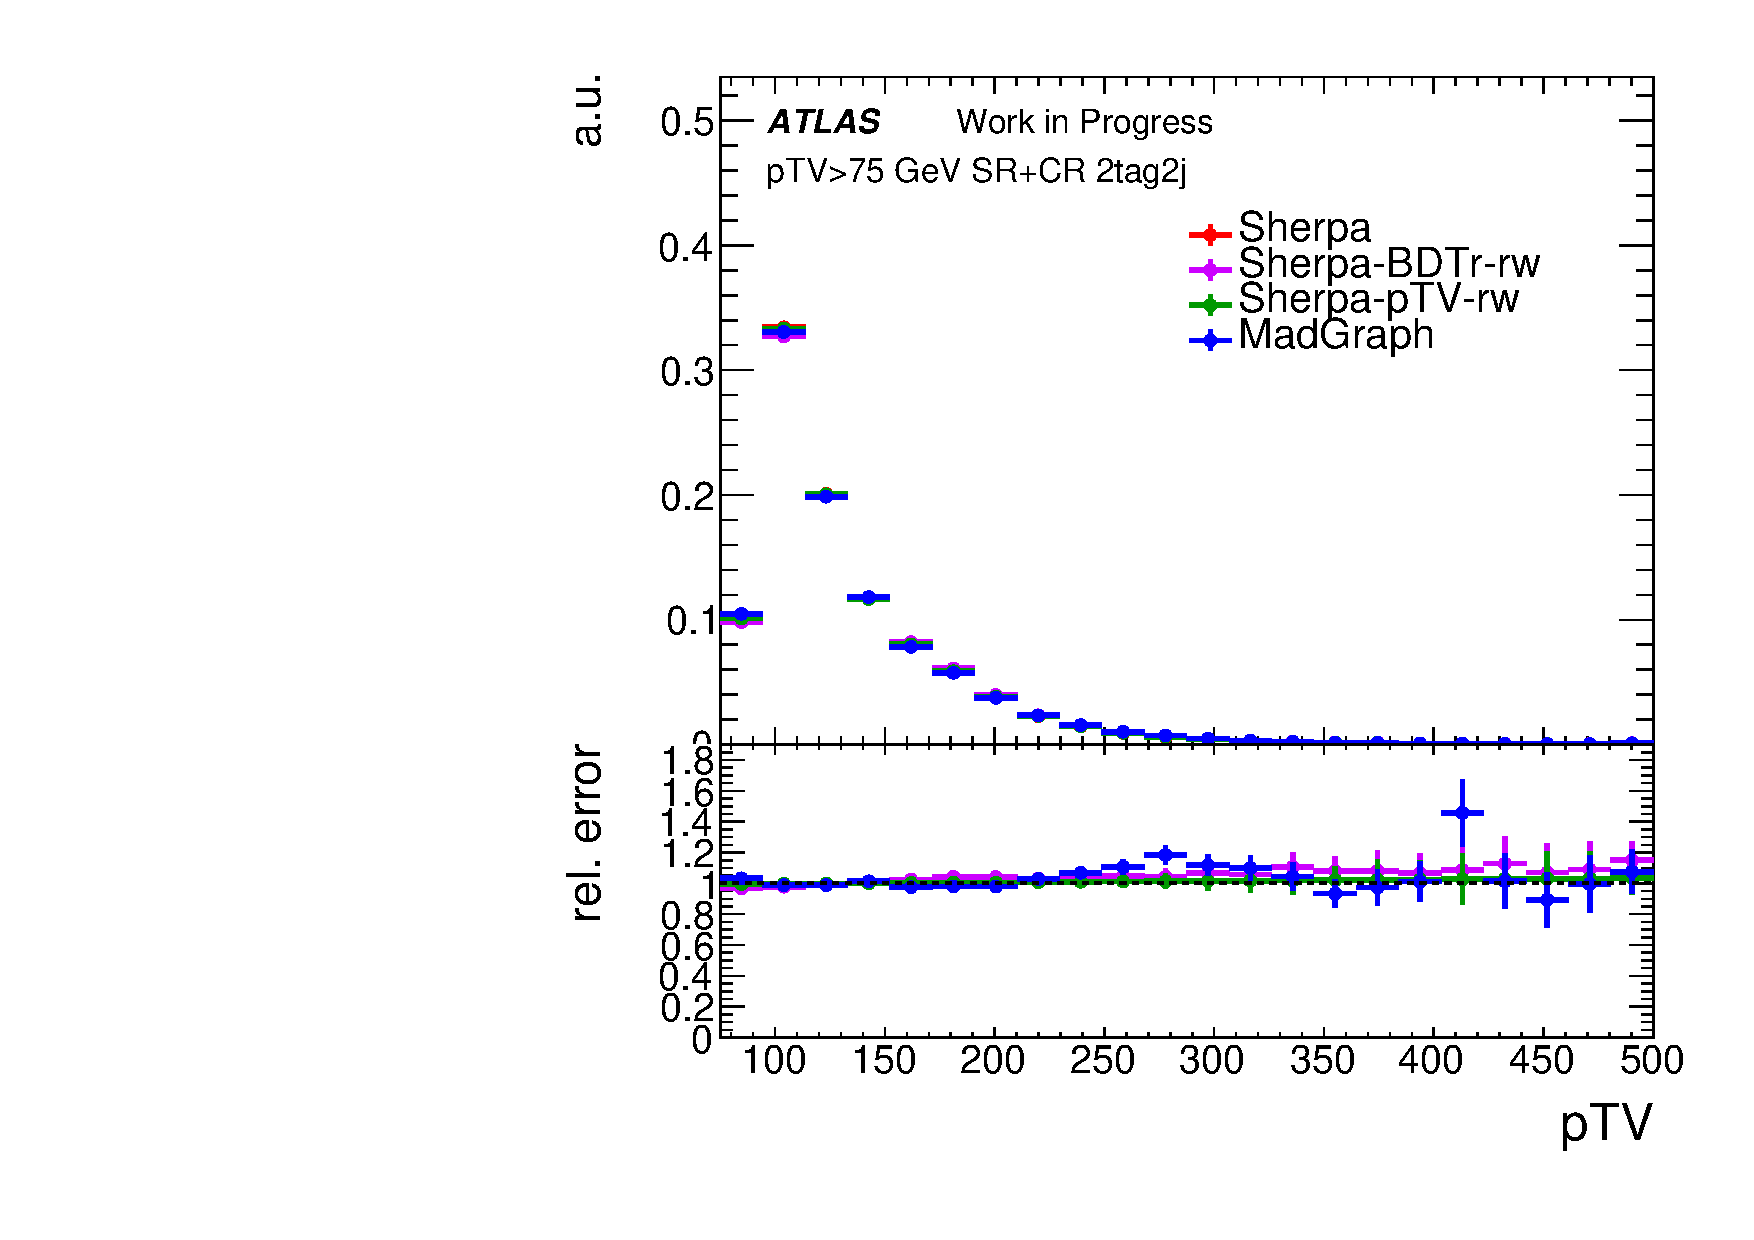
\includegraphics[width=0.45\textwidth]{1Lep_pTVreweighting_shapes/1lepton_2tag2jet_75ptv_SR+CR_pTV_bc.pdf}}\\
\subfloat[$bl$ events]{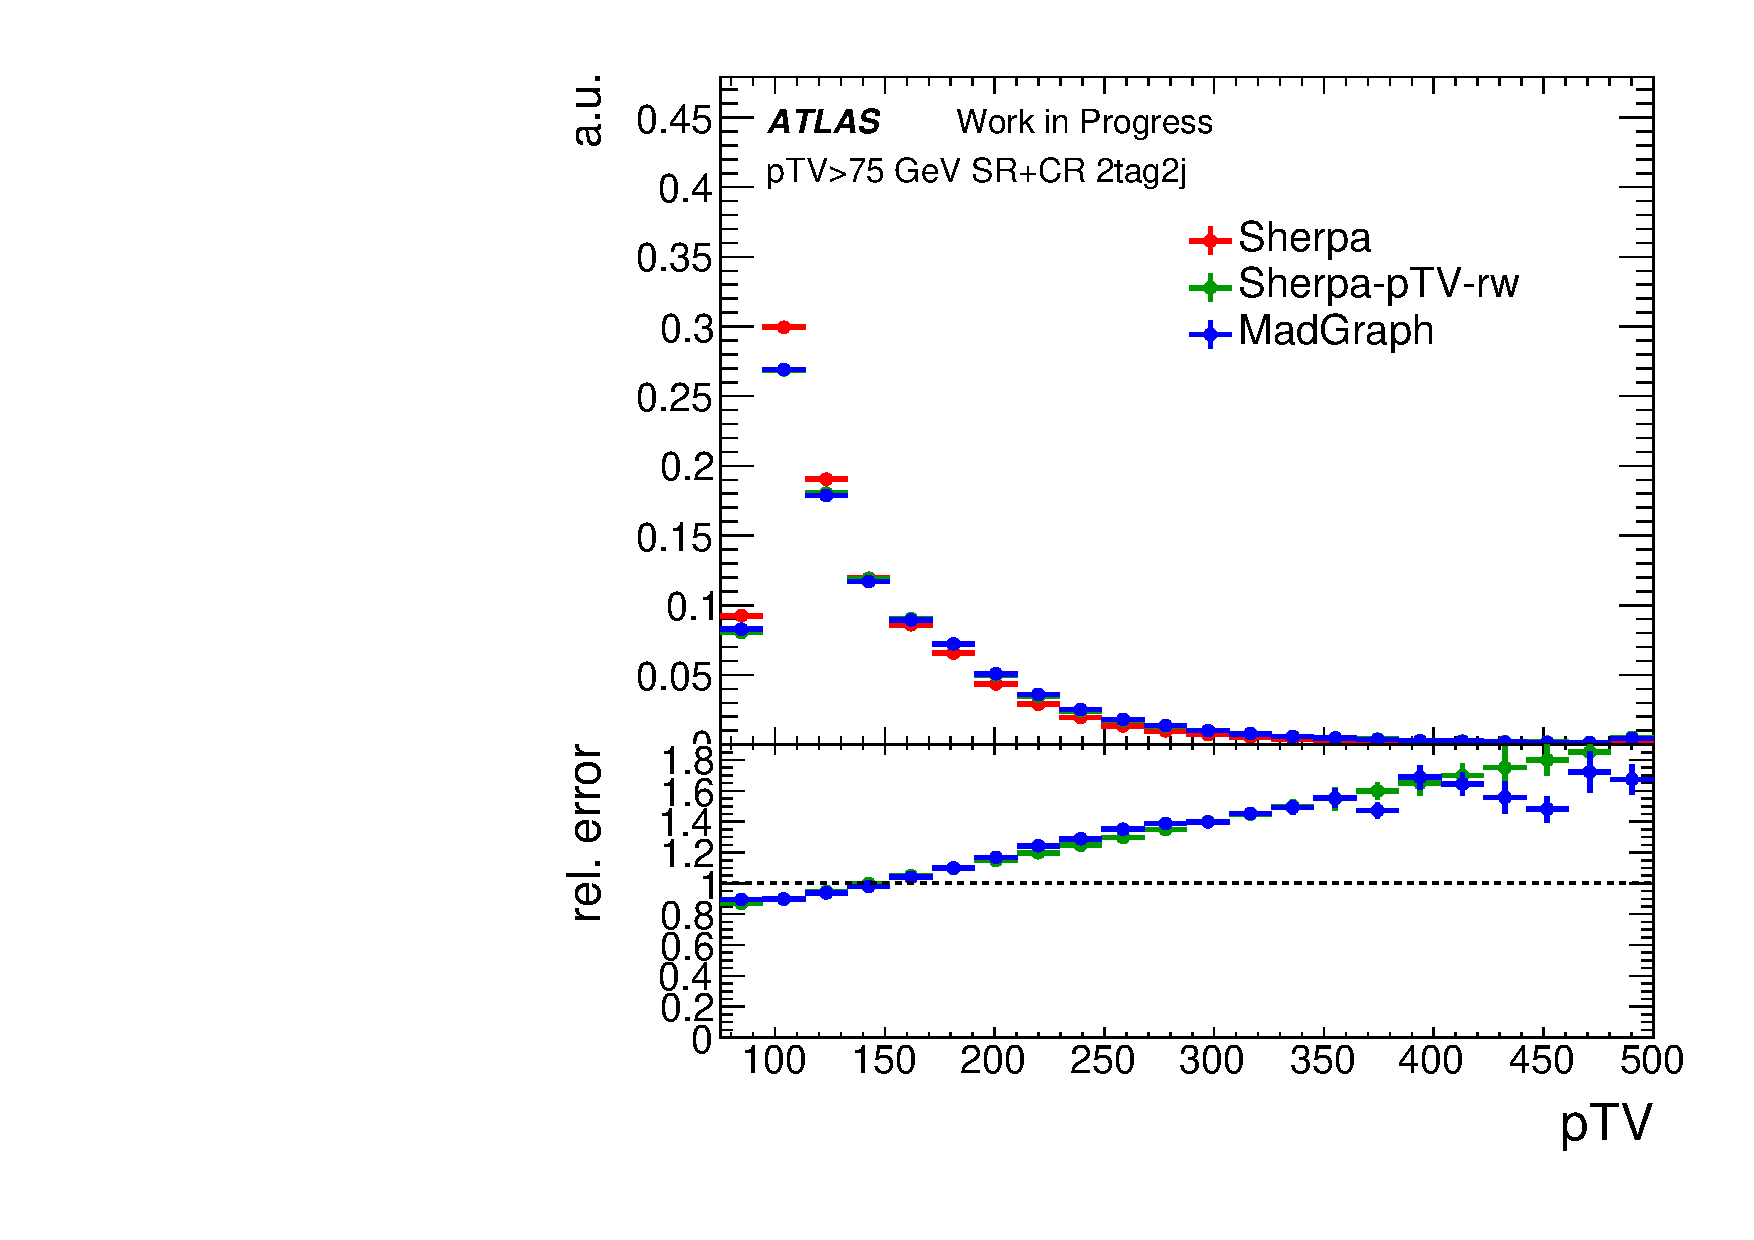
\includegraphics[width=0.45\textwidth]{1Lep_pTVreweighting_shapes/1lepton_2tag2jet_75ptv_SR+CR_pTV_bl.pdf}}&
\subfloat[Oth. events]{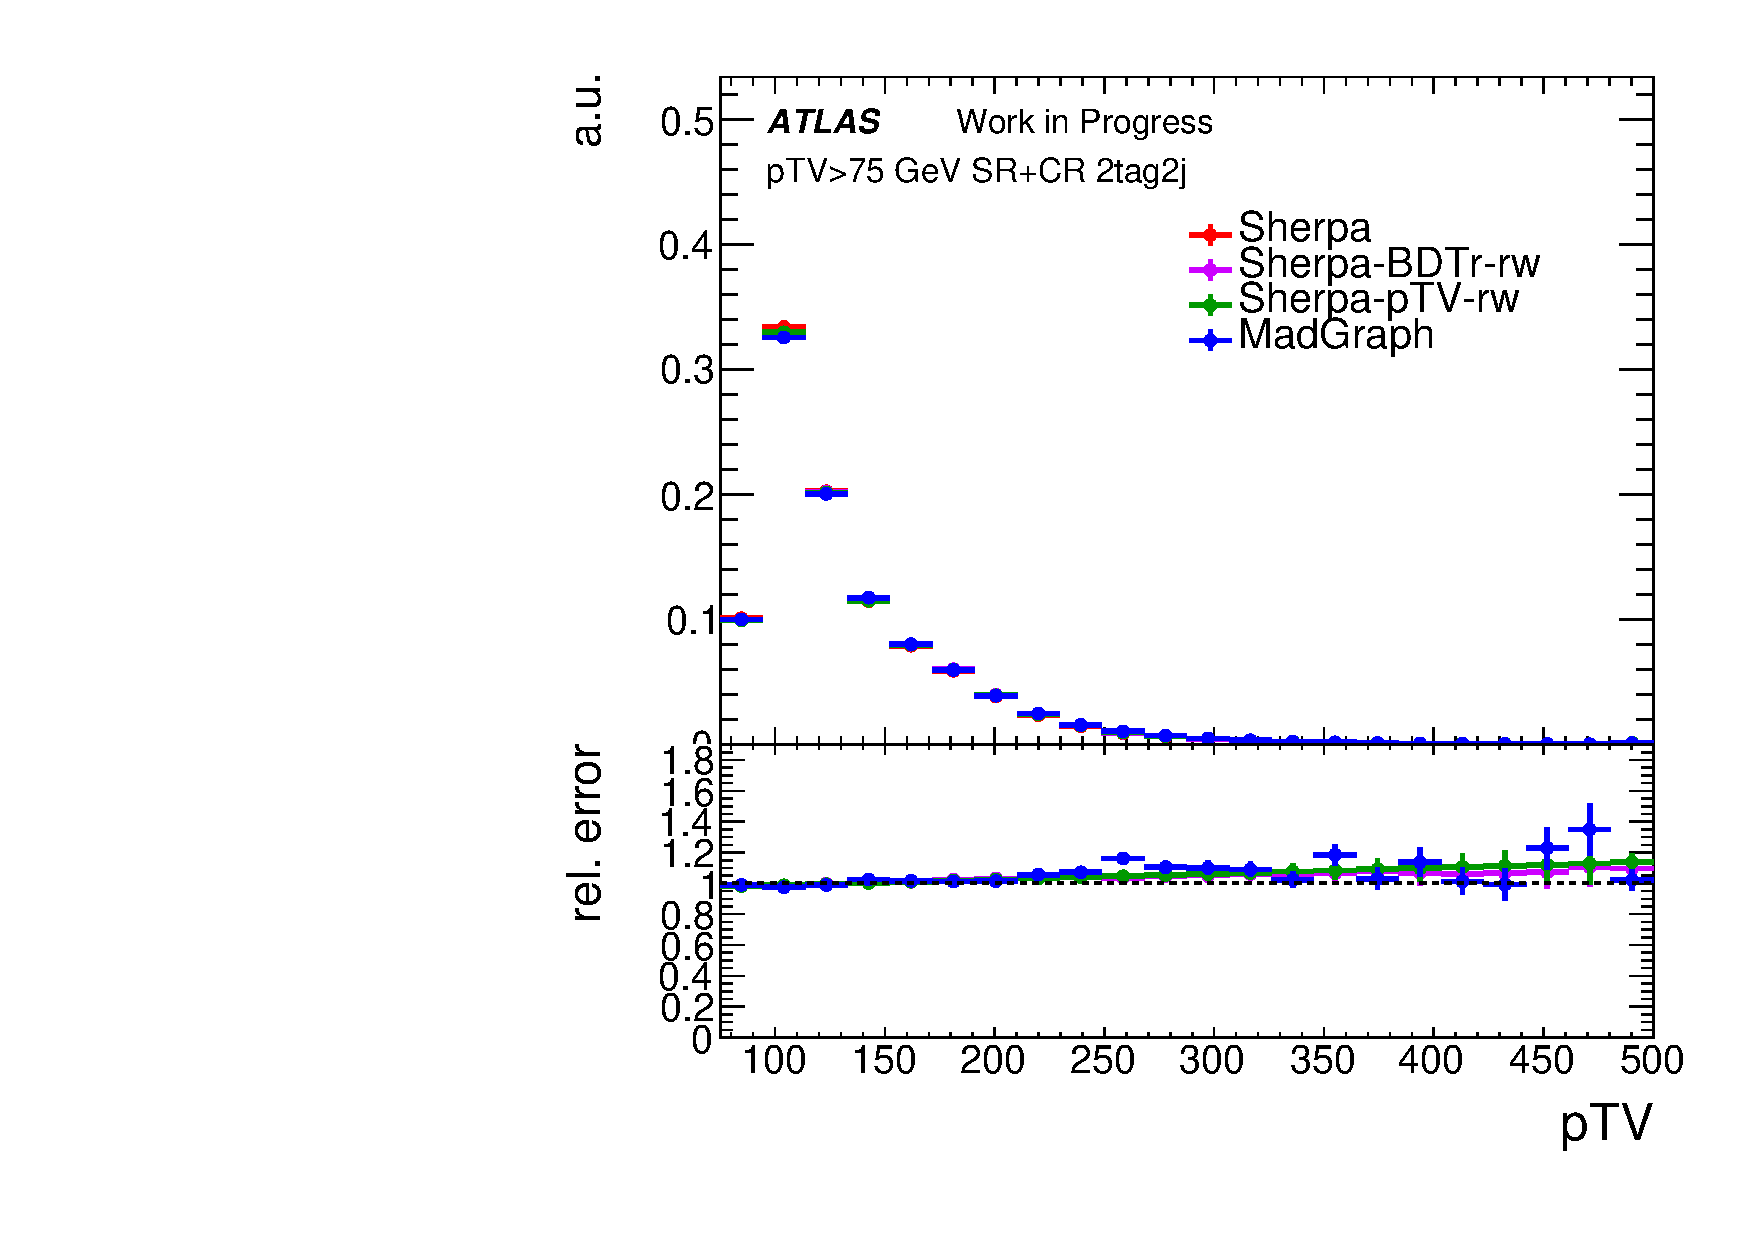
\includegraphics[width=0.45\textwidth]{1Lep_pTVreweighting_shapes/1lepton_2tag2jet_75ptv_SR+CR_pTV_cc.pdf}}\\
    \end{tabular}
    \caption[Derivation of $p_{\mathrm{T}}^V$ shape uncertainties on $W+$jets
events in the 1--lepton channel (2--jet category).]{$p_{\mathrm{T}}^V$ shape
systematic in the 2--jet category in the 1--lepton channel for each heavy
flavour sub-component. The red and blue histograms correspond to the
$p_{\mathrm{T}}^V$ prediction of \textsc{Sherpa}~2.2.1 and \textsc{MadGraph}
respectively. The $p_{\mathrm{T}}^V$ shape systematic is plotted in green.}
    \label{fig:wjets_1lep_2jet_SysWPtVBDTr}
  \end{figure}%
\begin{figure}[ht!] \centering
  \begin{tabular}{cc} \subfloat[$bb$ events]{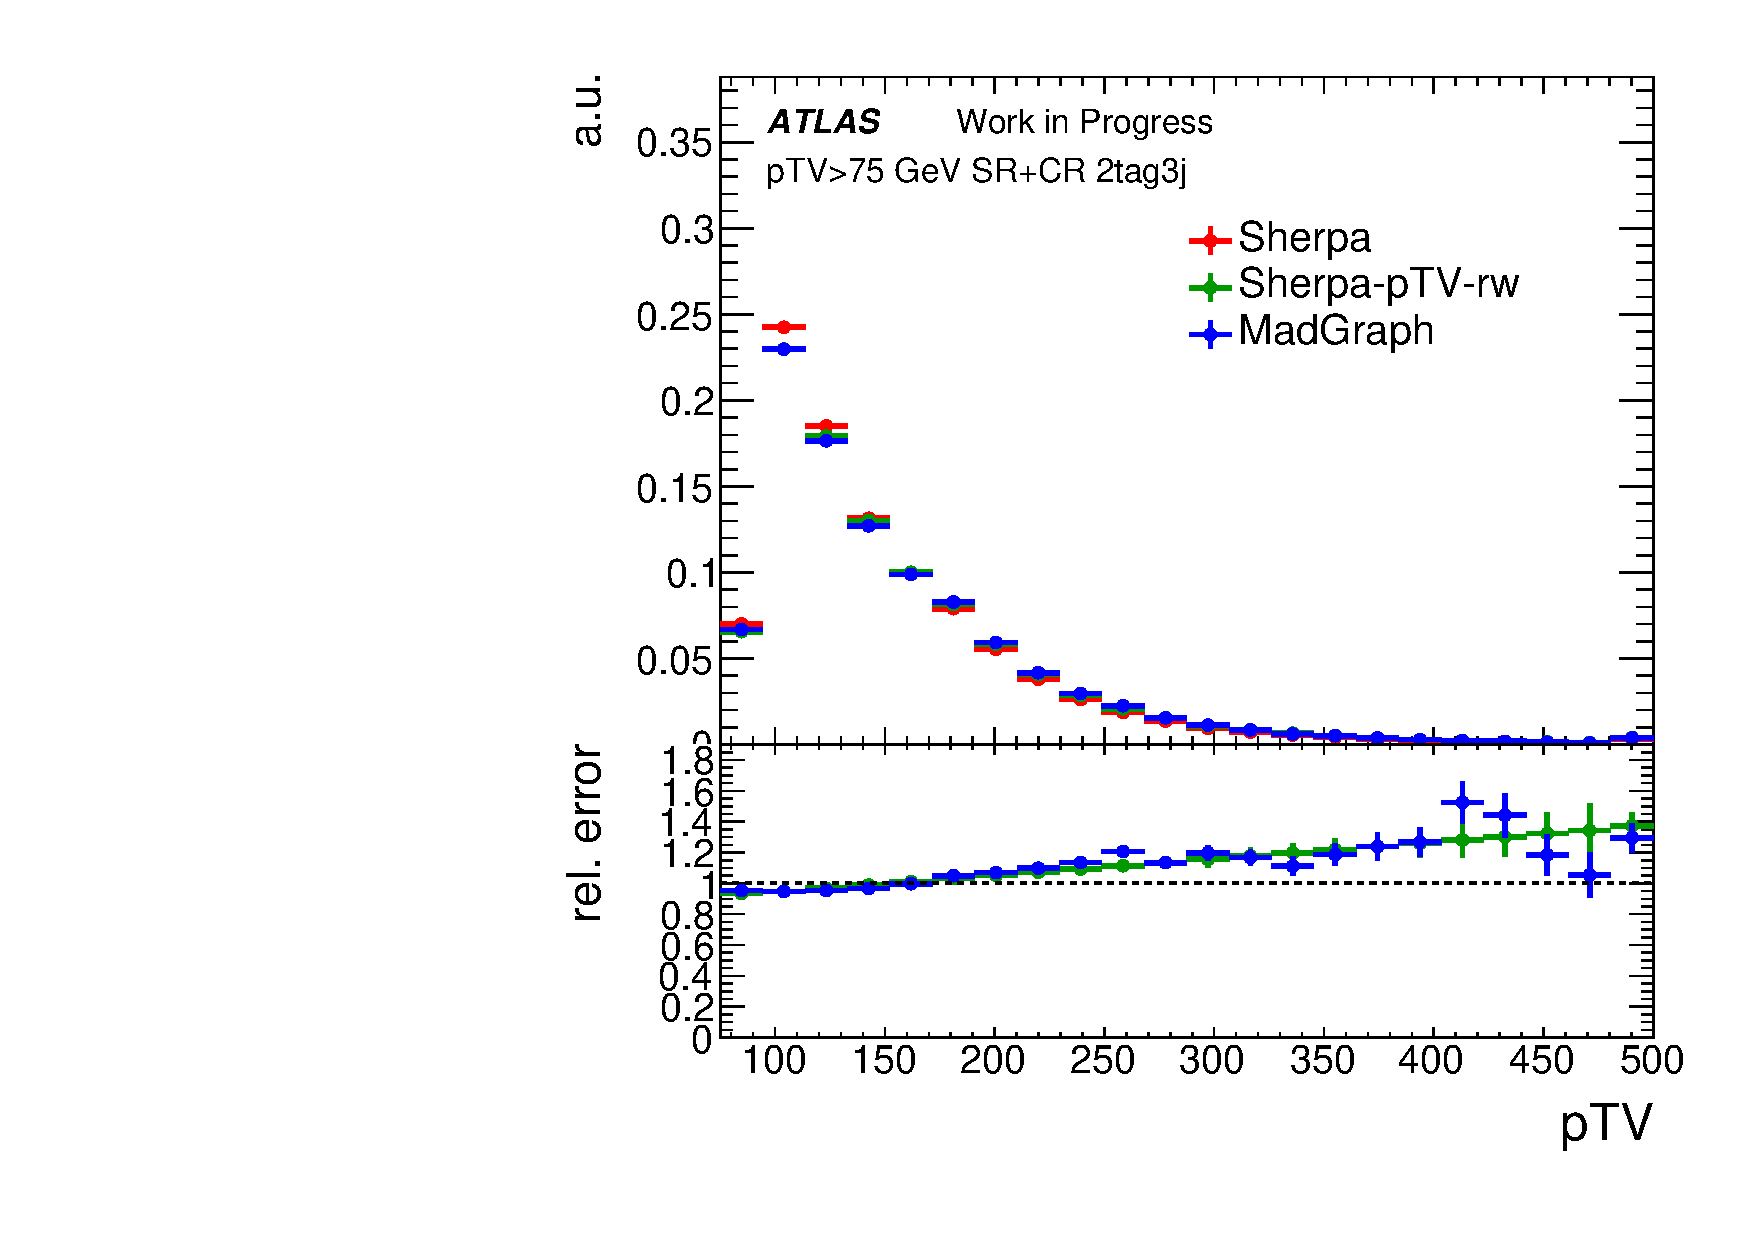
\includegraphics[width=0.45\textwidth]{1Lep_pTVreweighting_shapes/1lepton_2tag3jet_75ptv_SR+CR_pTV_bb.pdf}}&
\subfloat[$bc$ events]{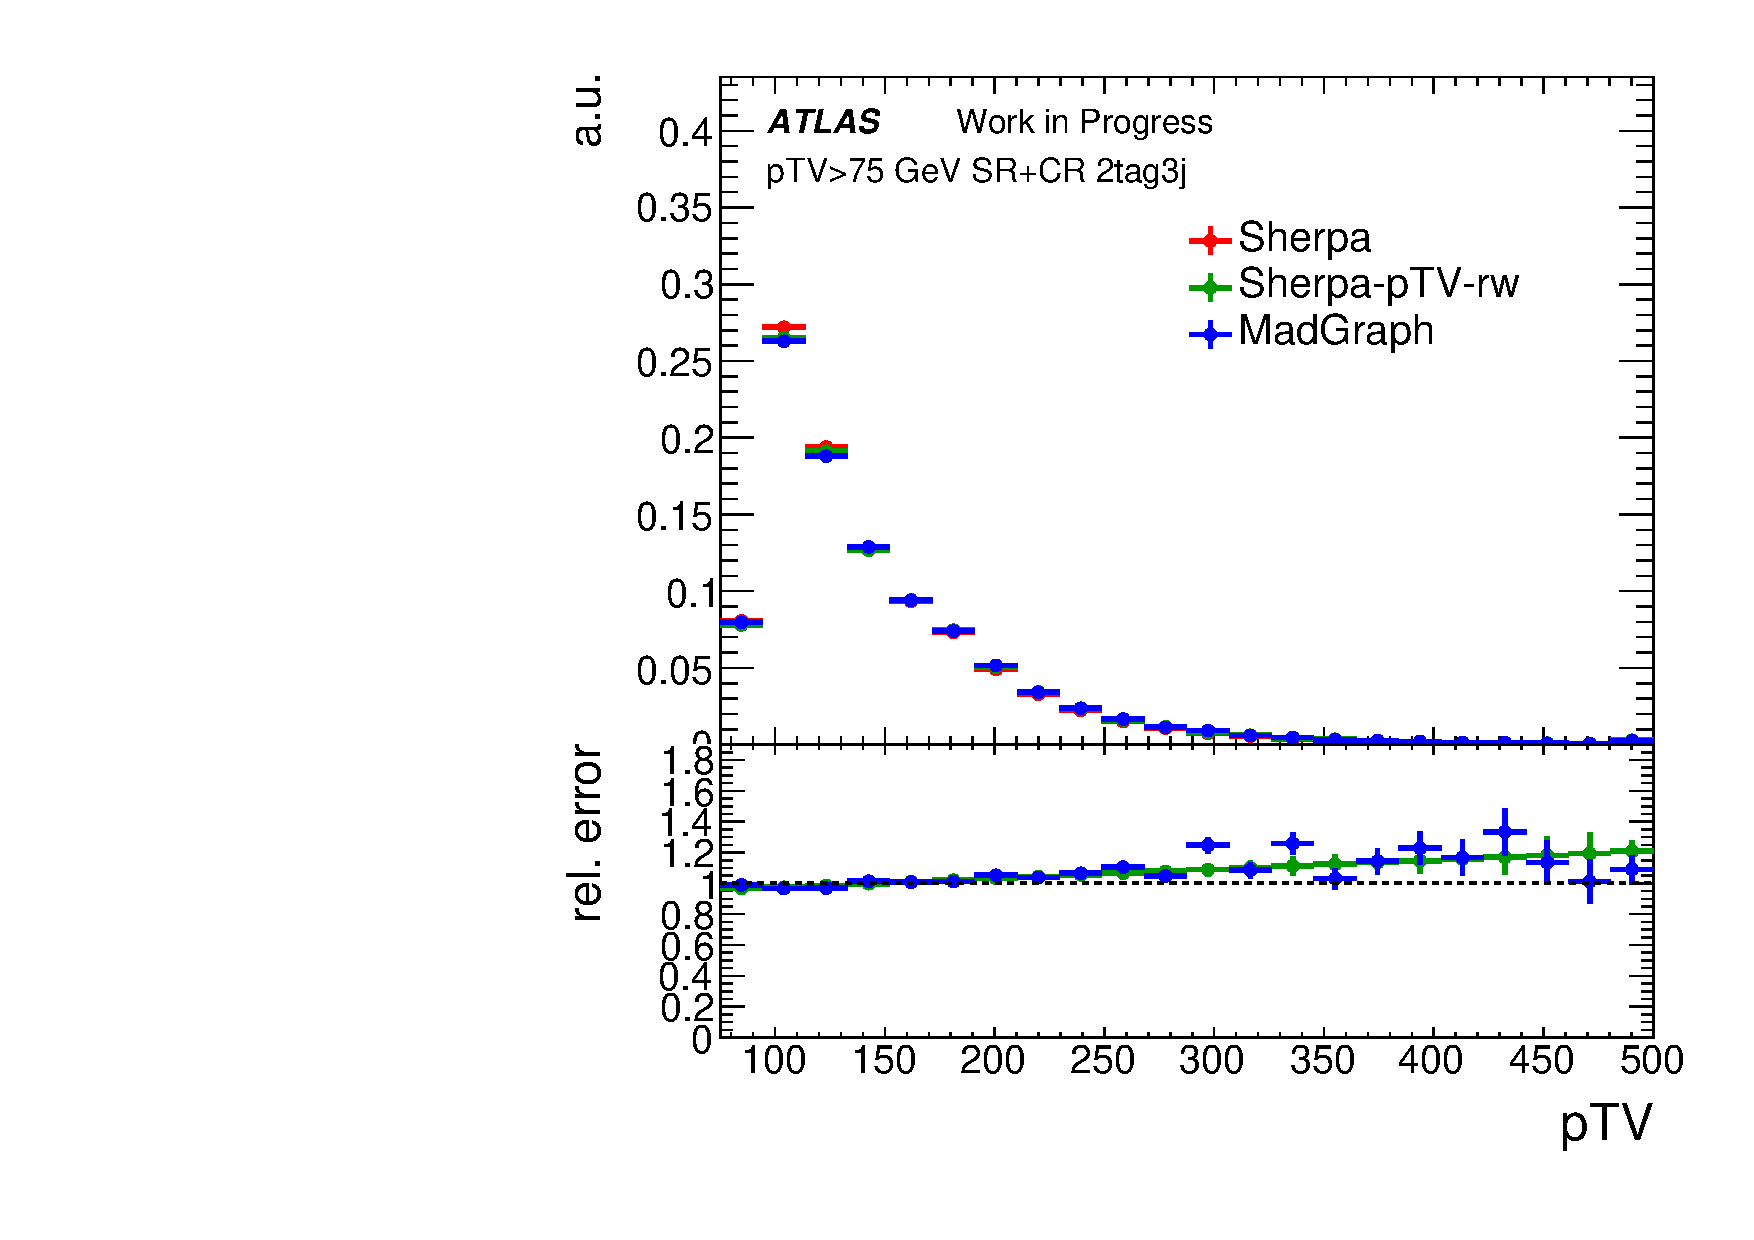
\includegraphics[width=0.45\textwidth]{1Lep_pTVreweighting_shapes/1lepton_2tag3jet_75ptv_SR+CR_pTV_bc.pdf}}\\
\subfloat[$bl$ events]{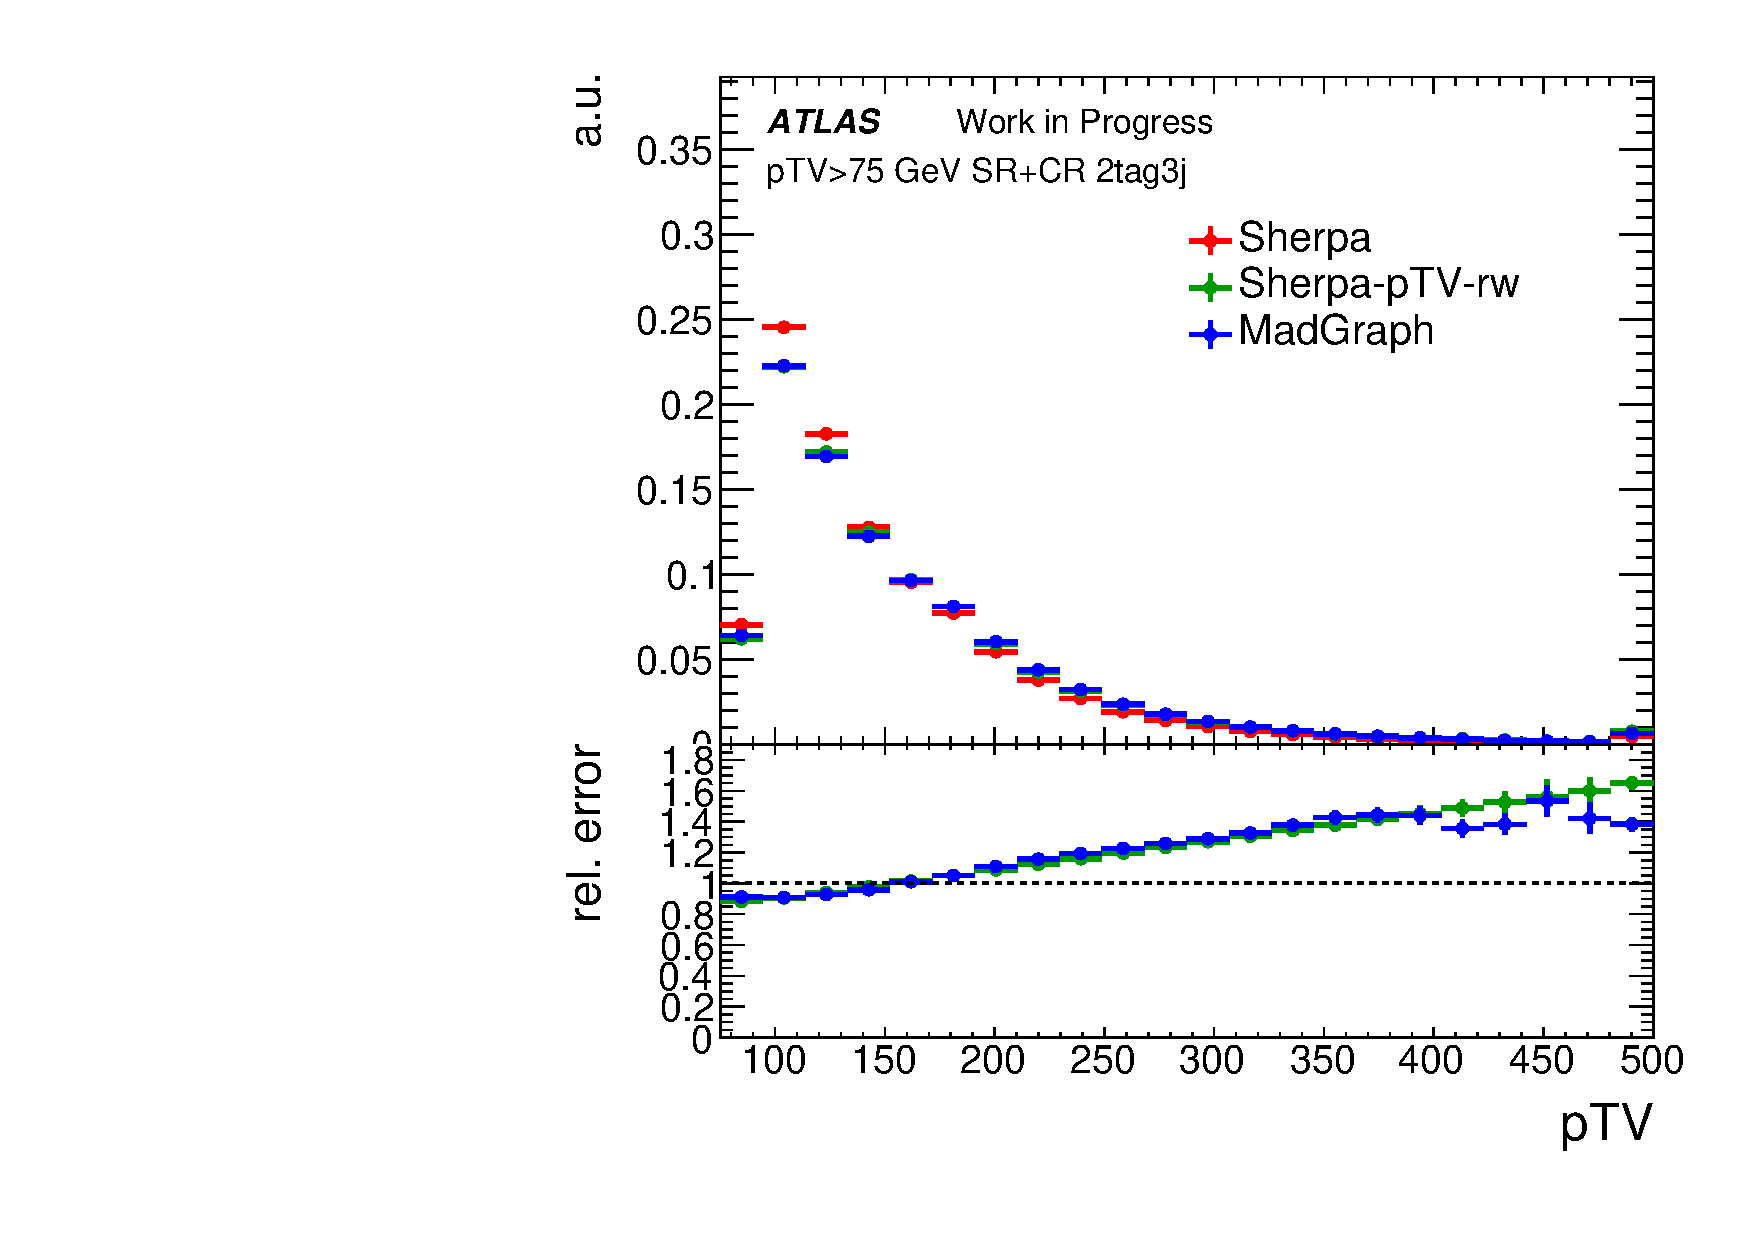
\includegraphics[width=0.45\textwidth]{1Lep_pTVreweighting_shapes/1lepton_2tag3jet_75ptv_SR+CR_pTV_bl.pdf}}&
\subfloat[Oth. events]{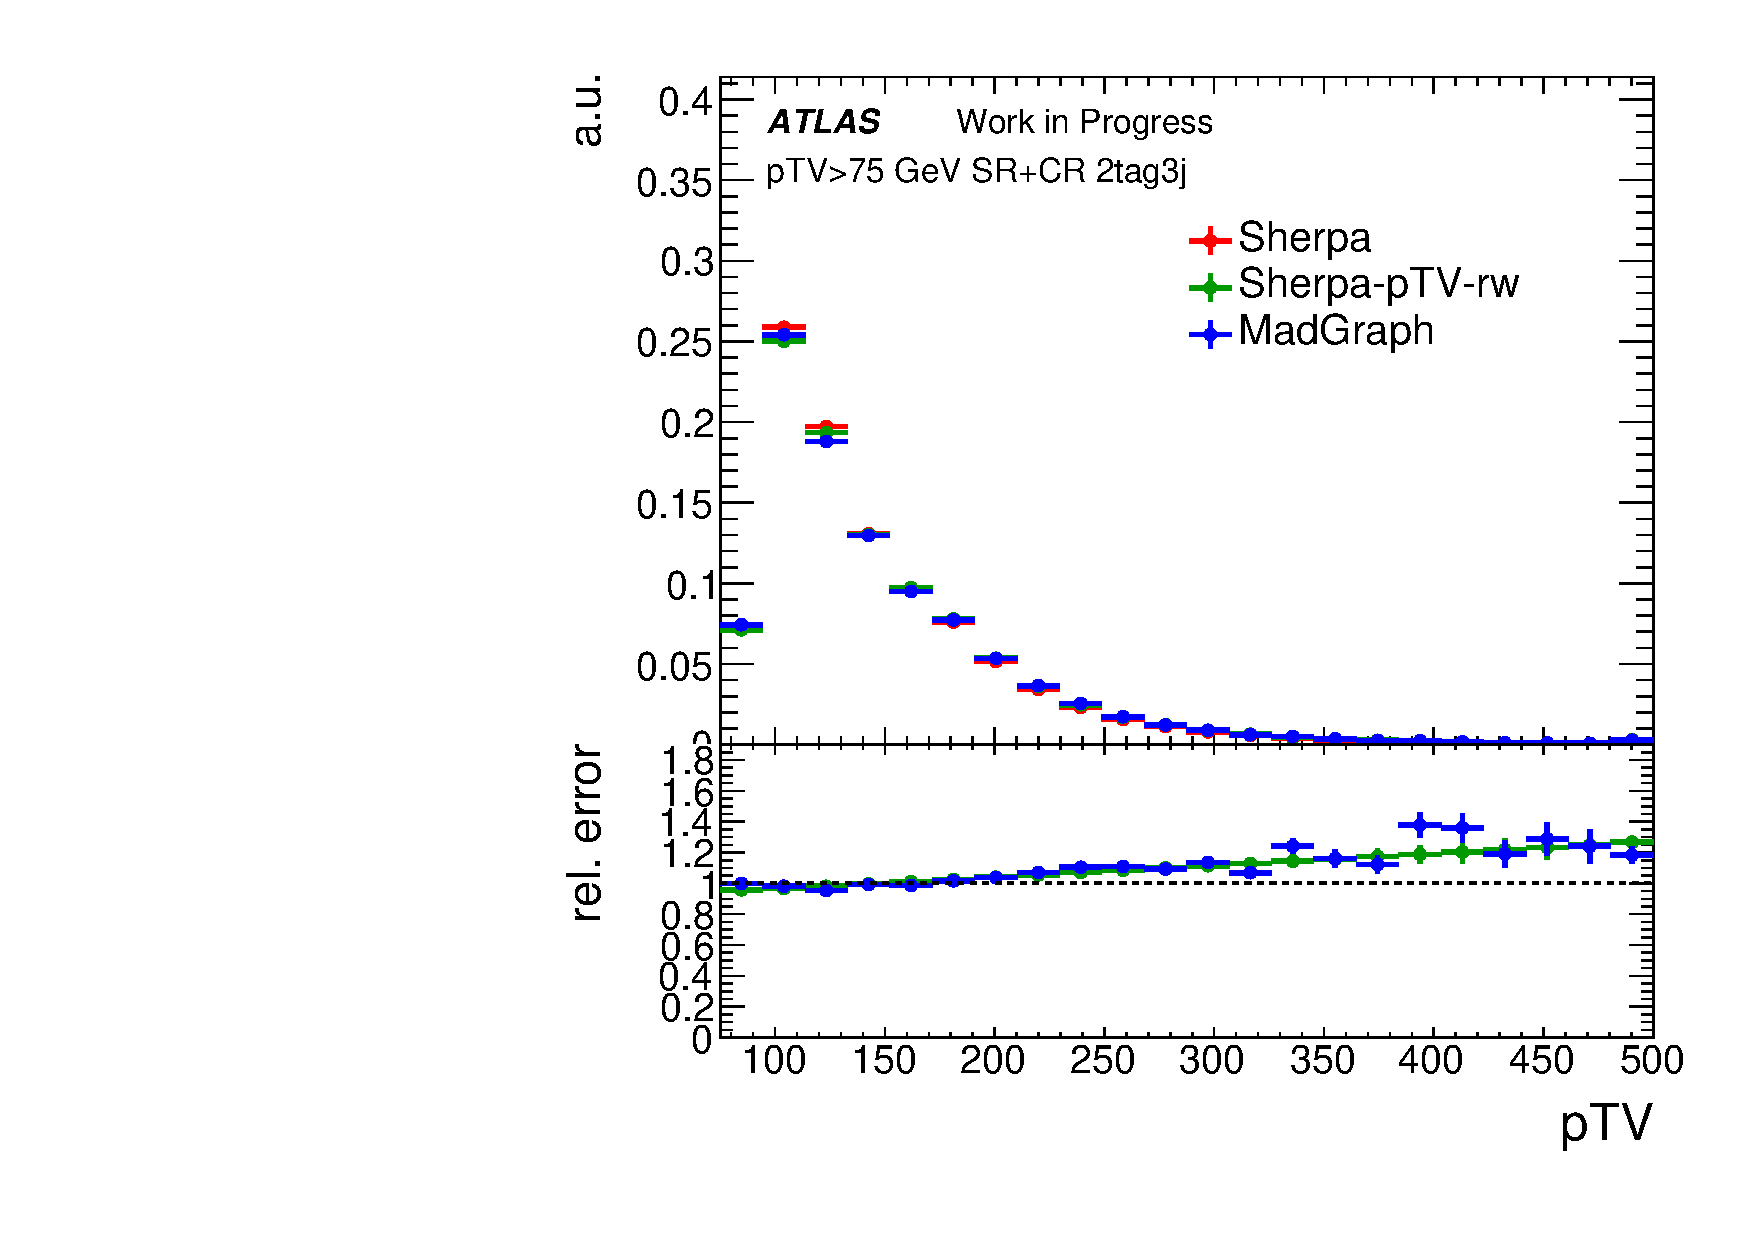
\includegraphics[width=0.45\textwidth]{1Lep_pTVreweighting_shapes/1lepton_2tag3jet_75ptv_SR+CR_pTV_cc.pdf}}\\
  \end{tabular}
  \caption[Derivation of $p_{\mathrm{T}}^V$ shape uncertainties on $W+$jets
events in the 1--lepton channel (3--jet category).]{$p_{\mathrm{T}}^V$ shape
systematic in the 3--jet category in the 1--lepton channel for each heavy
flavour sub-component. The red and blue histograms correspond to the
$p_{\mathrm{T}}^V$ prediction of \textsc{Sherpa}~2.2.1 and \textsc{MadGraph}
respectively. The $p_{\mathrm{T}}^V$ shape systematic is plotted in green.}
  \label{fig:wjets_1lep_3jet_SysWPtVBDTr}
\end{figure}
The systematic uncertainties on the shape are shown in the ratio panel at the
bottom of each plot in green.

The low number of events available in the 0--lepton channel mean that it is not
statistically viable to generate a parametrisation in that channel, therefore
the shapes derived in the 1--lepton channel are also used in the 0--lepton
channel. Figure~\ref{fig:wjets_01lep_2jet_SysWPtVBDTr}
and~\ref{fig:wjets_01lep_3jet_SysWPtVBDTr} show a comparison of the $p_T^V$
shapes derived in the 1--lepton channel compared with the equivalent systematic
derived in the 0--lepton channel in the $E_T^{\text{miss}}$ variable for the 2--
and 3--jet categories, respectively.
\begin{figure}[ht!]
  \centering
  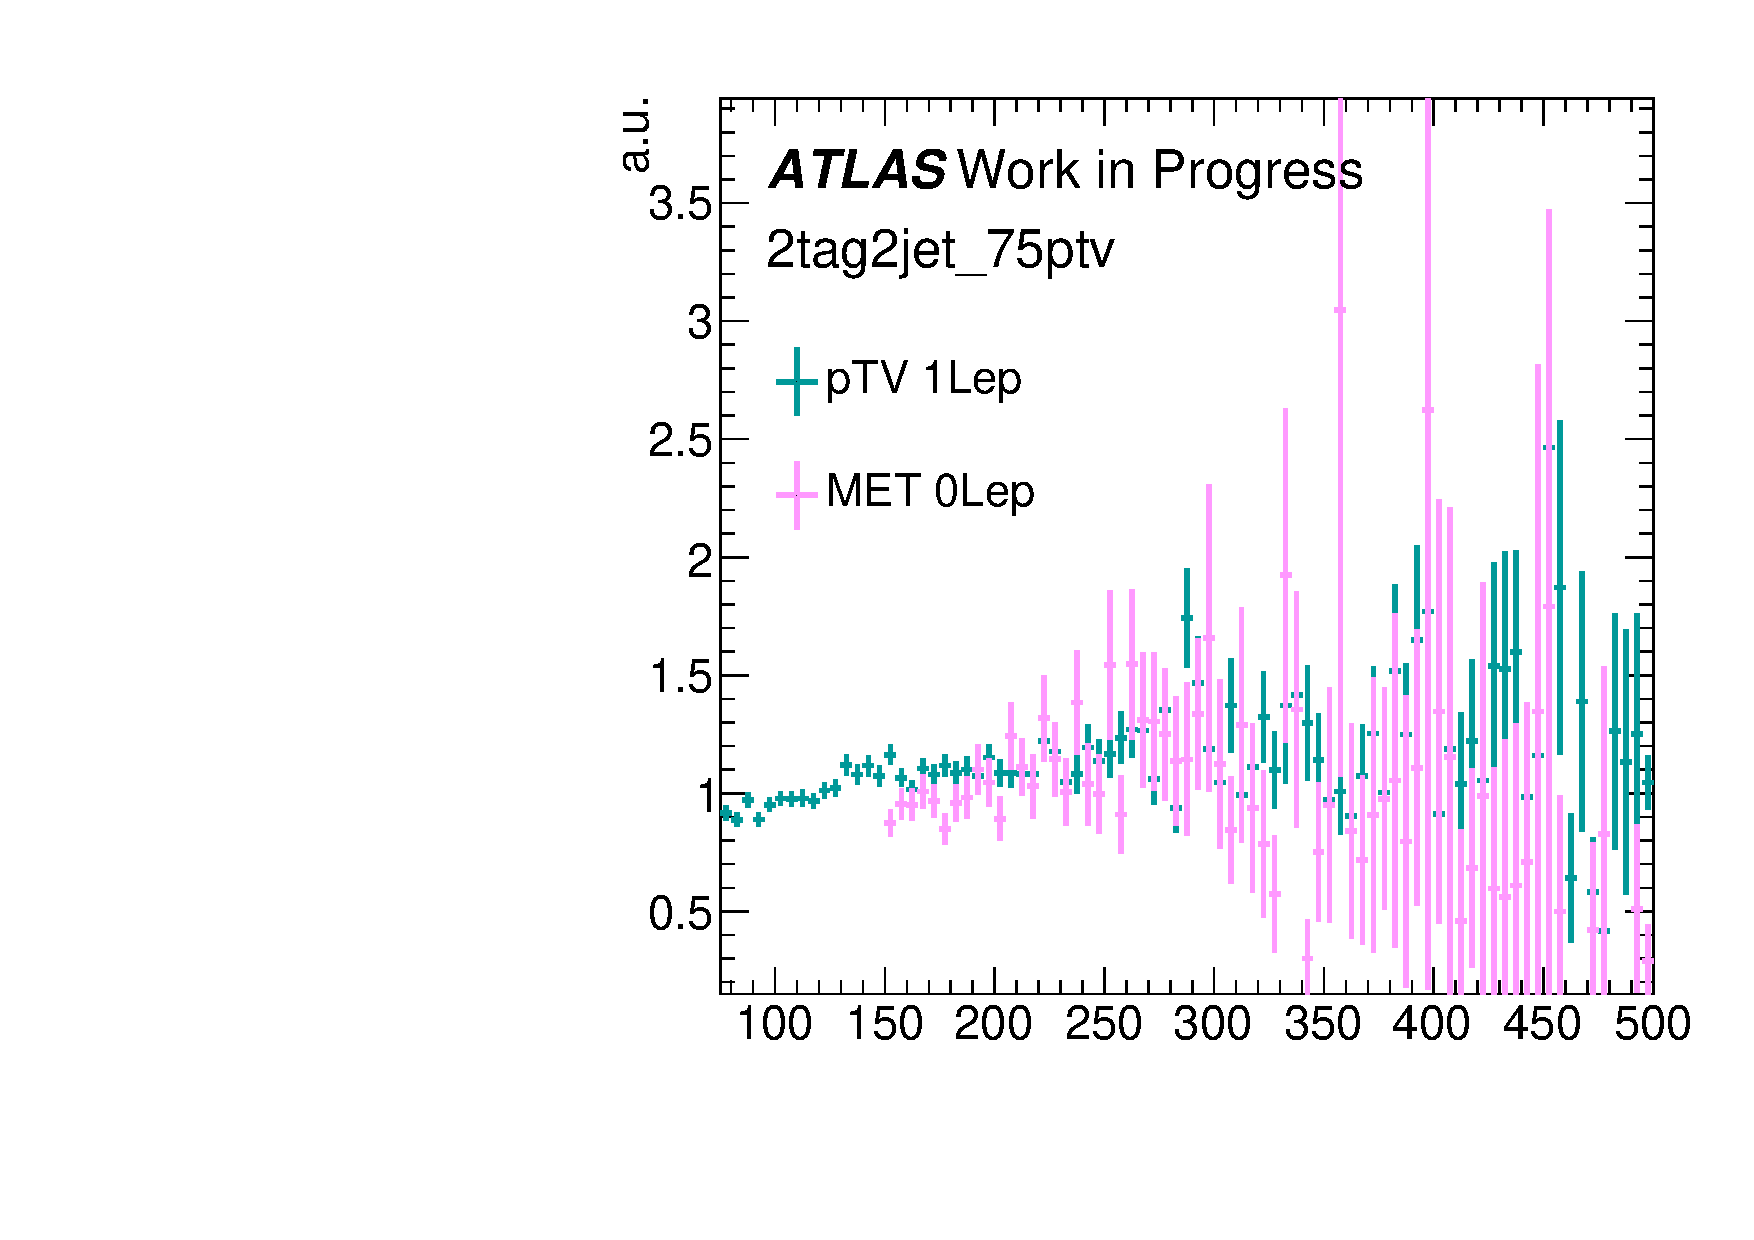
\includegraphics[width=0.45\textwidth]{01Lep_reweighting_shapes/ReweightingVarComparison_2tag2jet_75ptv_bb.pdf}
  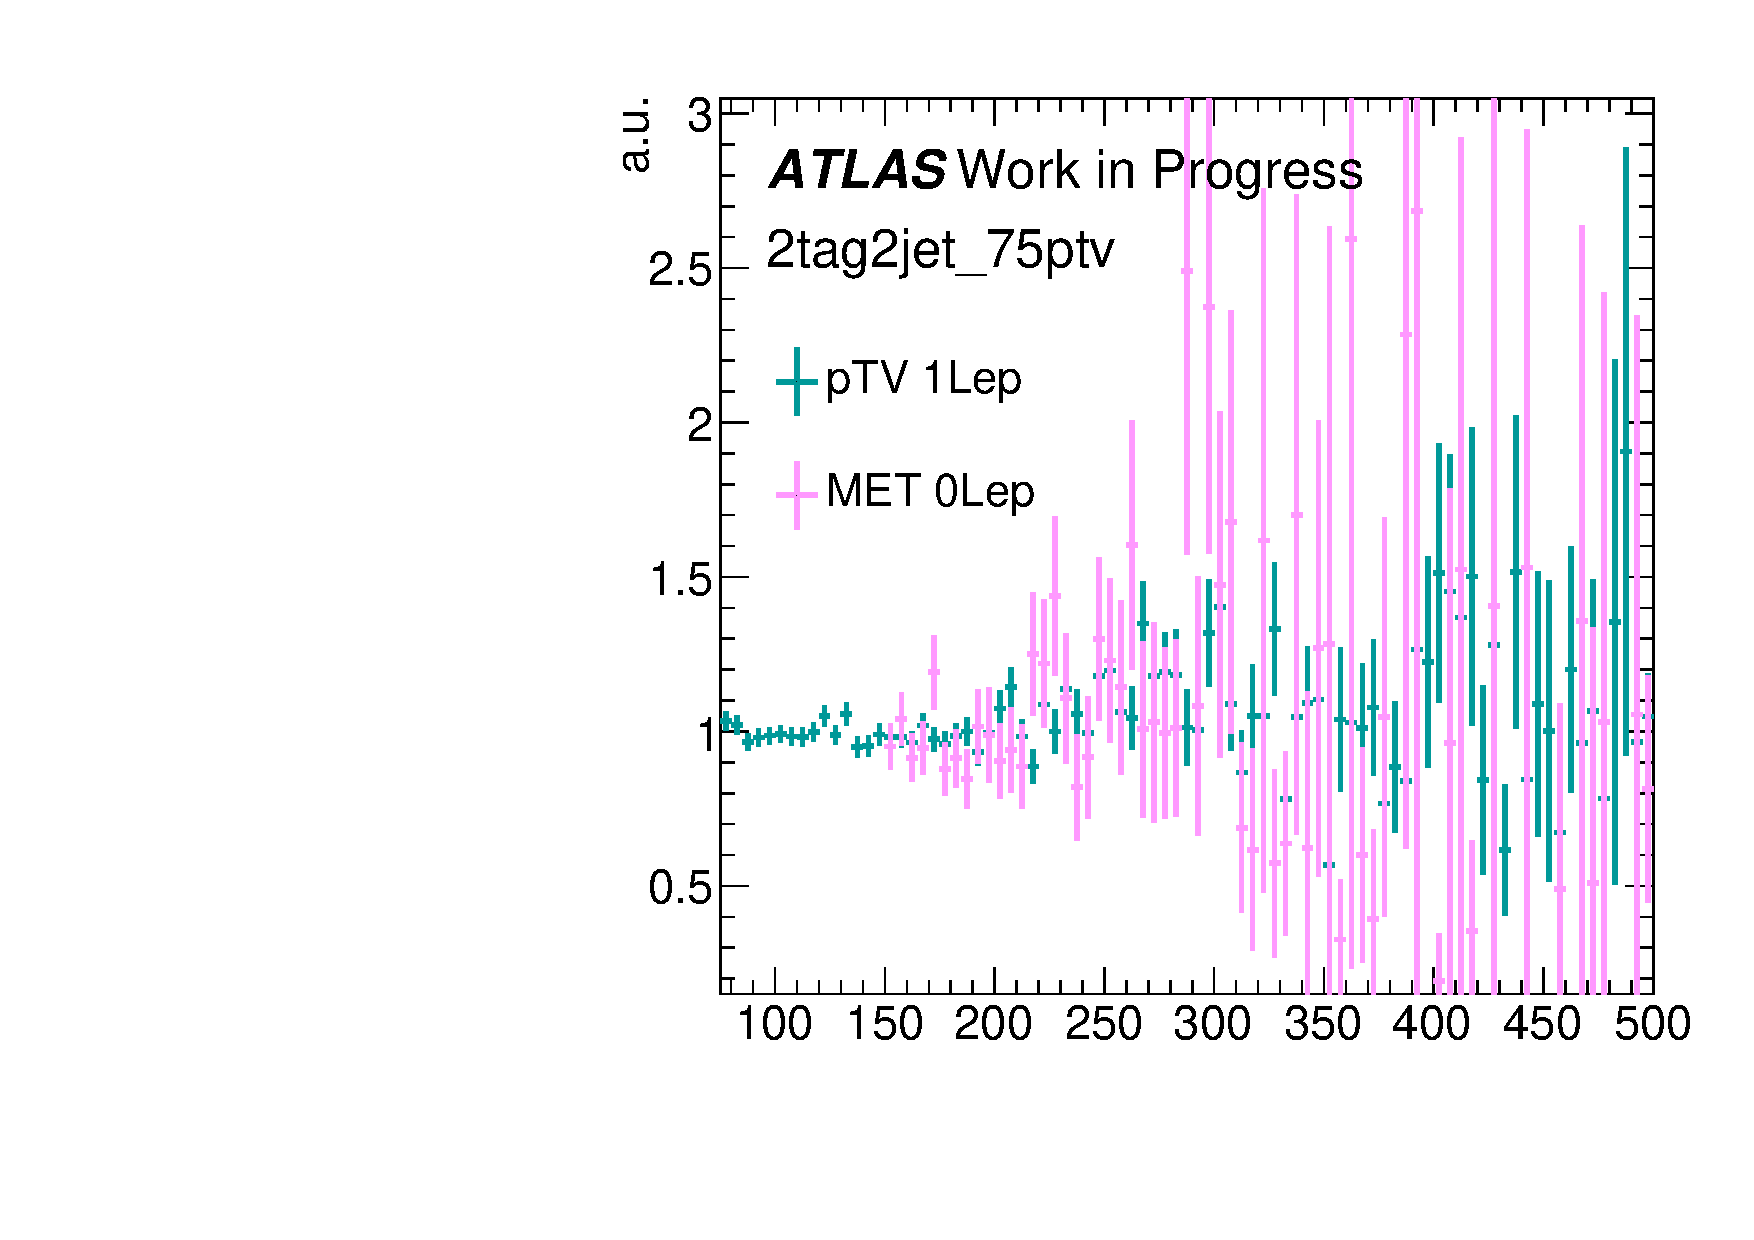
\includegraphics[width=0.45\textwidth]{01Lep_reweighting_shapes/ReweightingVarComparison_2tag2jet_75ptv_bc.pdf}
  \\
  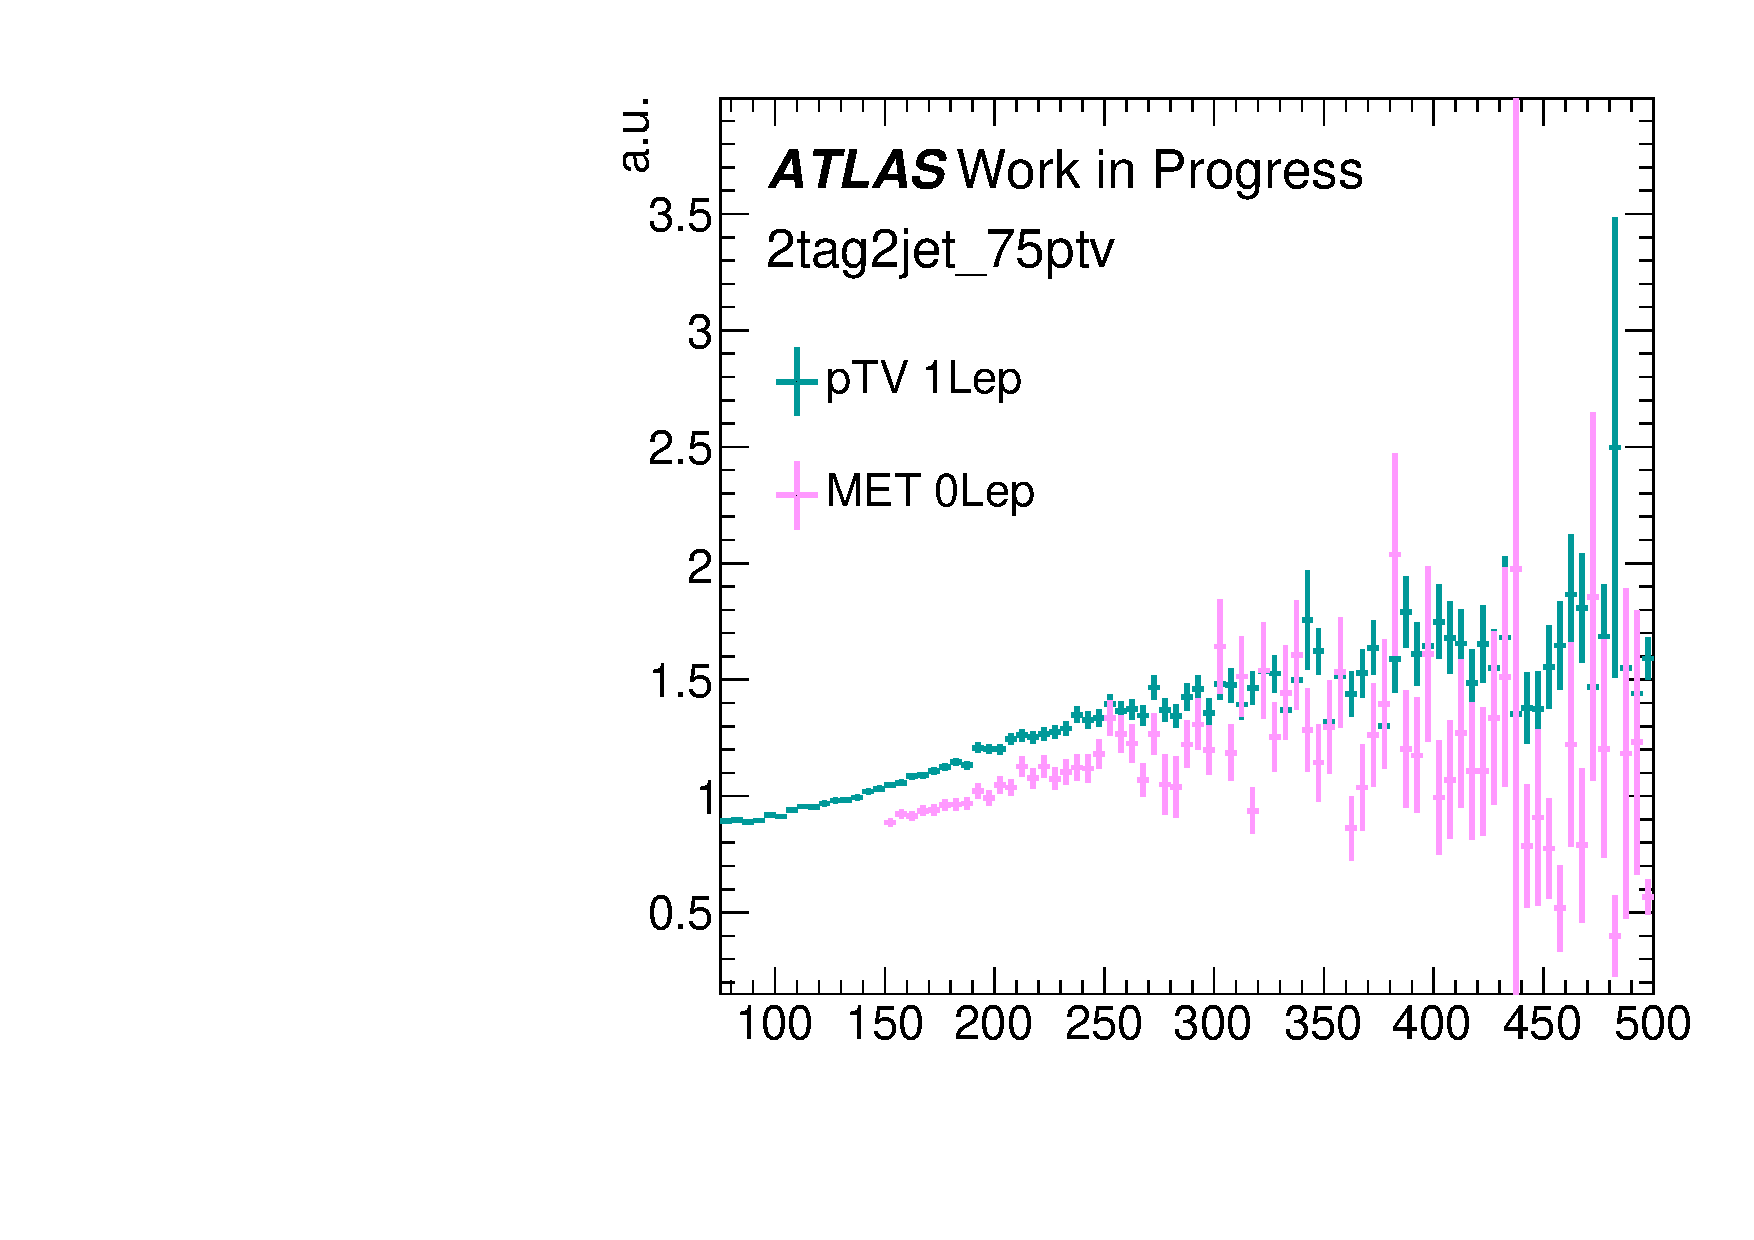
\includegraphics[width=0.45\textwidth]{01Lep_reweighting_shapes/ReweightingVarComparison_2tag2jet_75ptv_bl.pdf}
  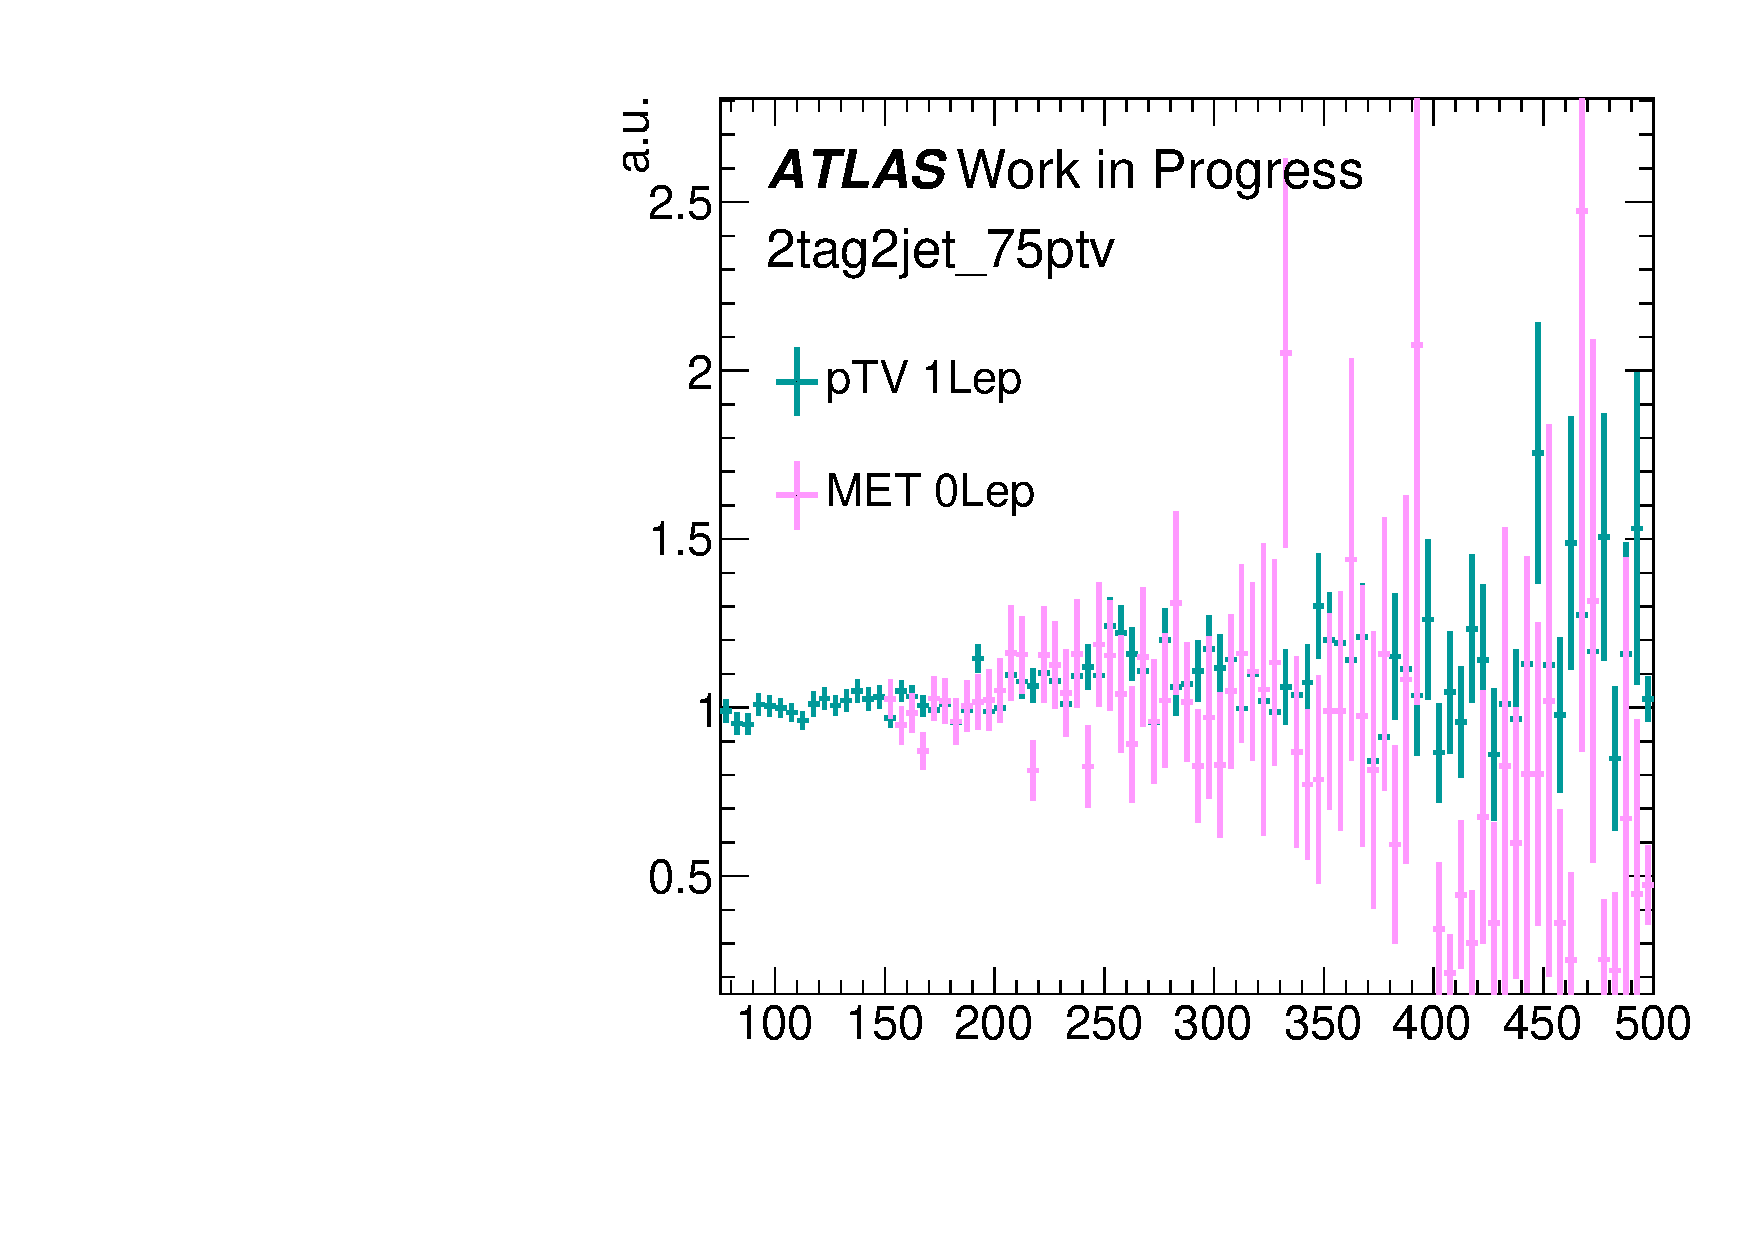
\includegraphics[width=0.45\textwidth]{01Lep_reweighting_shapes/ReweightingVarComparison_2tag2jet_75ptv_cc.pdf}
  \\
  \caption{$p_T^V$ and $E_T^{\text{miss}}$ shape systematics derived in the
    2--jet region of the 1-- and 0--lepton channels, respectively, for each
    heavy flavour sub-component.}
  
  \label{fig:wjets_01lep_2jet_SysWPtVBDTr}
\end{figure}

\begin{figure}[ht!]
  \centering
  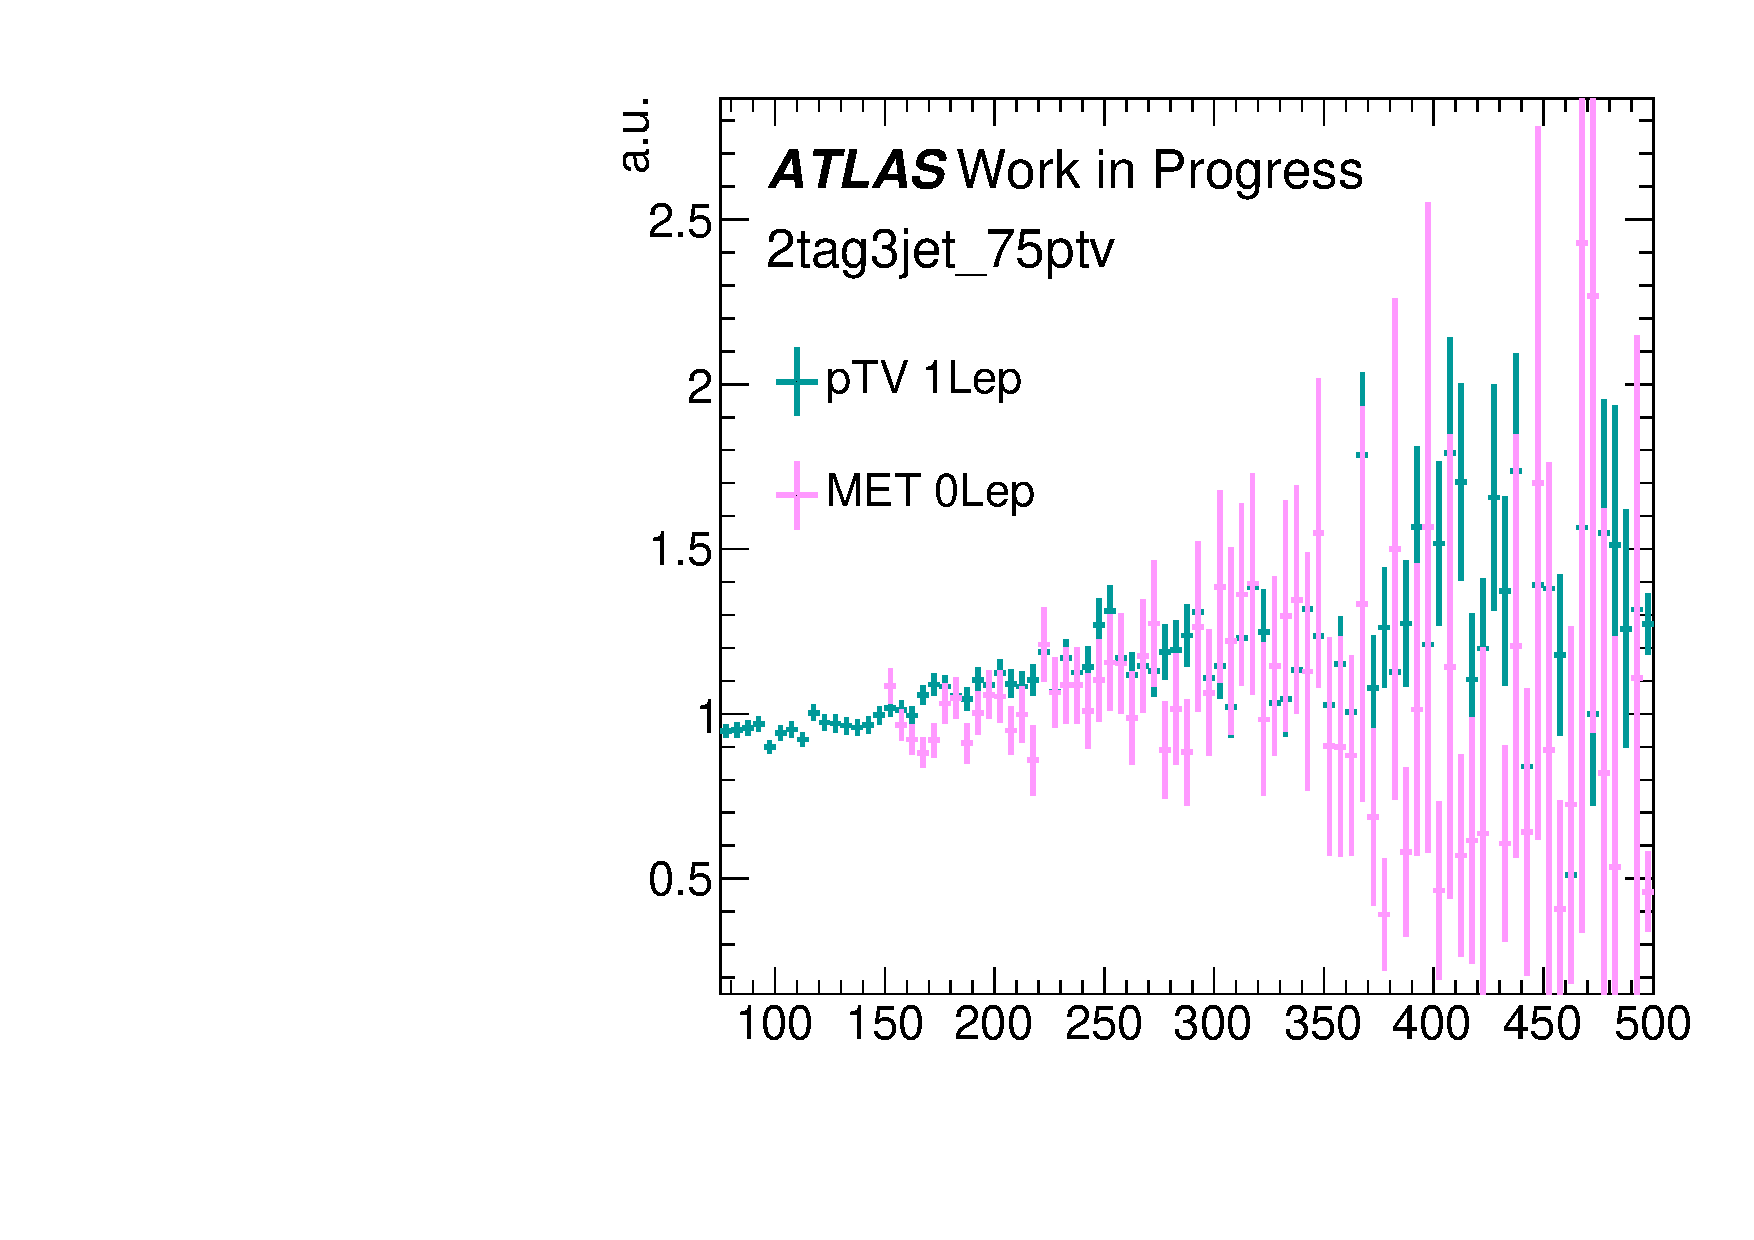
\includegraphics[width=0.45\textwidth]{01Lep_reweighting_shapes/ReweightingVarComparison_2tag3jet_75ptv_bb.pdf}
  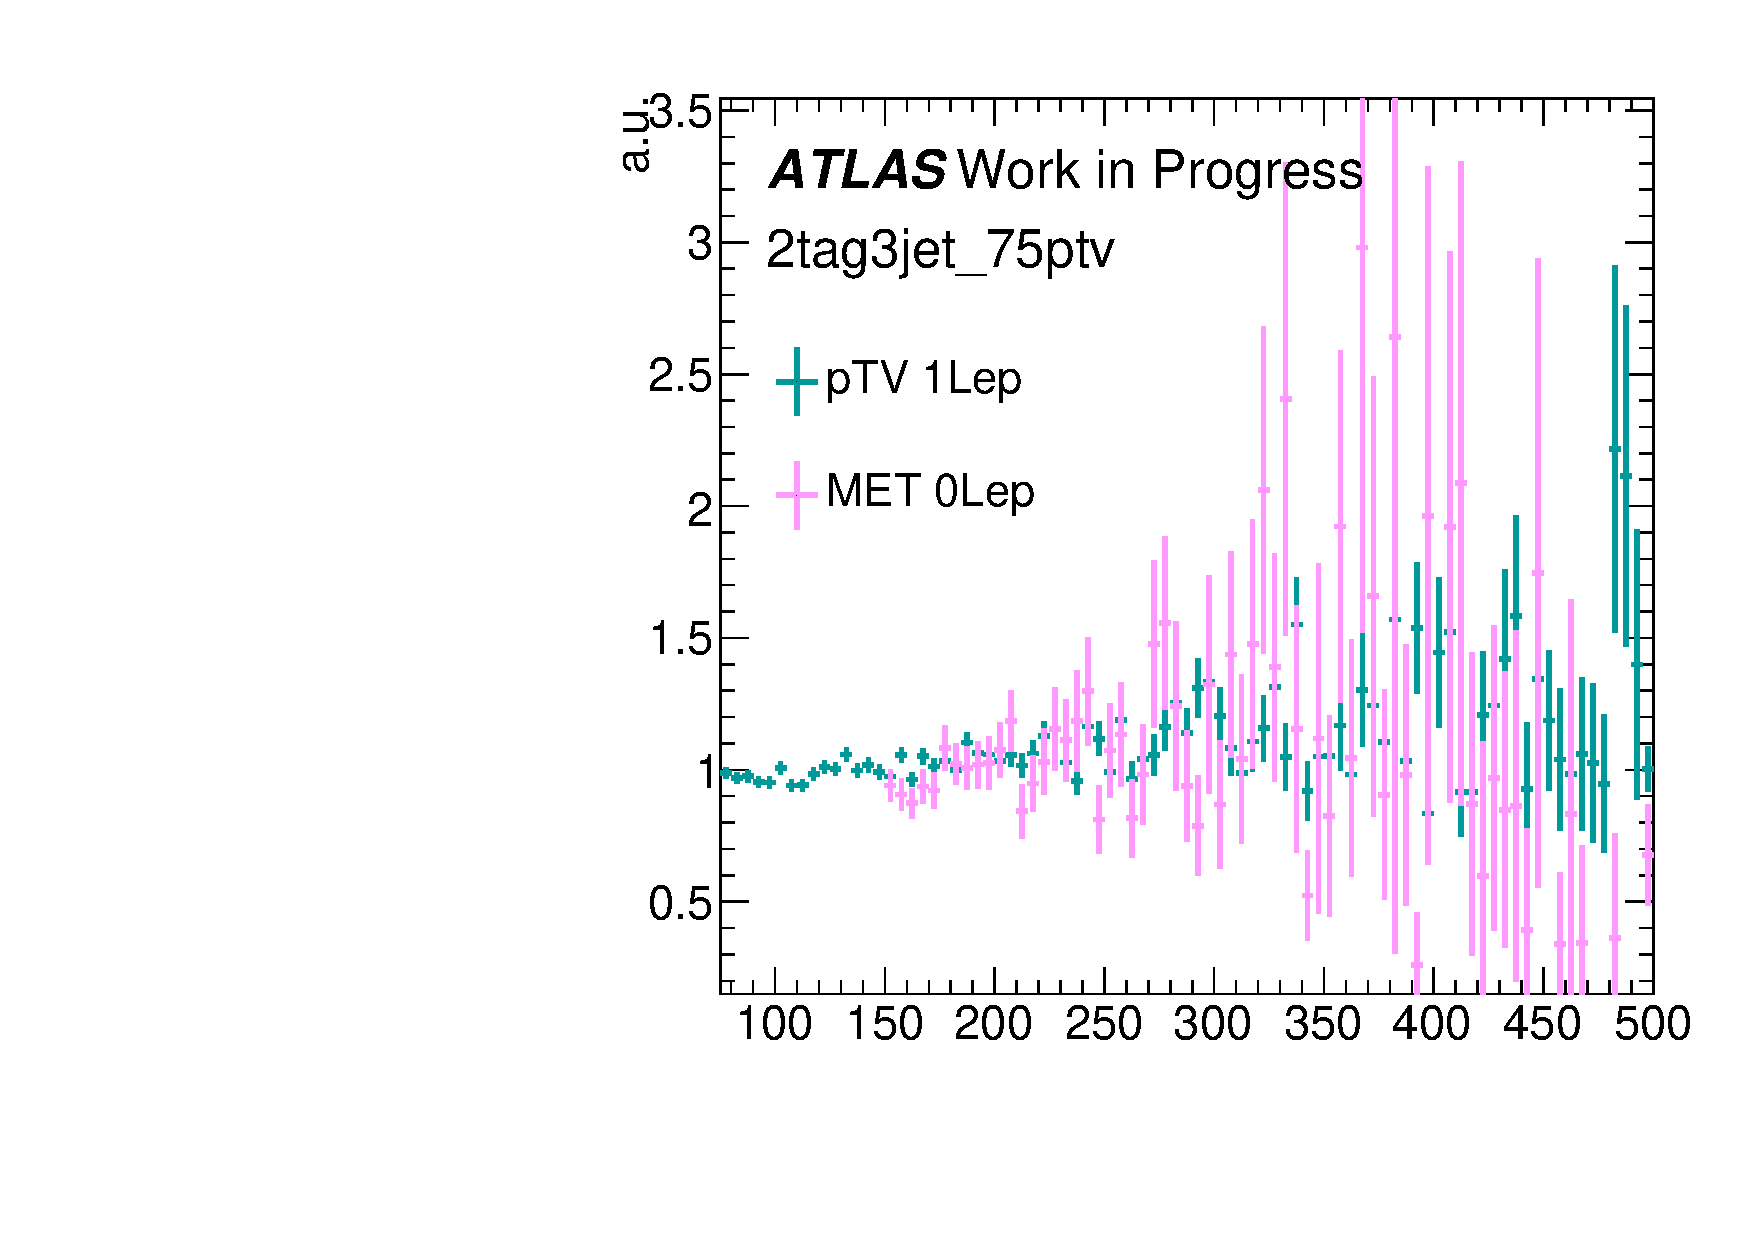
\includegraphics[width=0.45\textwidth]{01Lep_reweighting_shapes/ReweightingVarComparison_2tag3jet_75ptv_bc.pdf}
  \\
  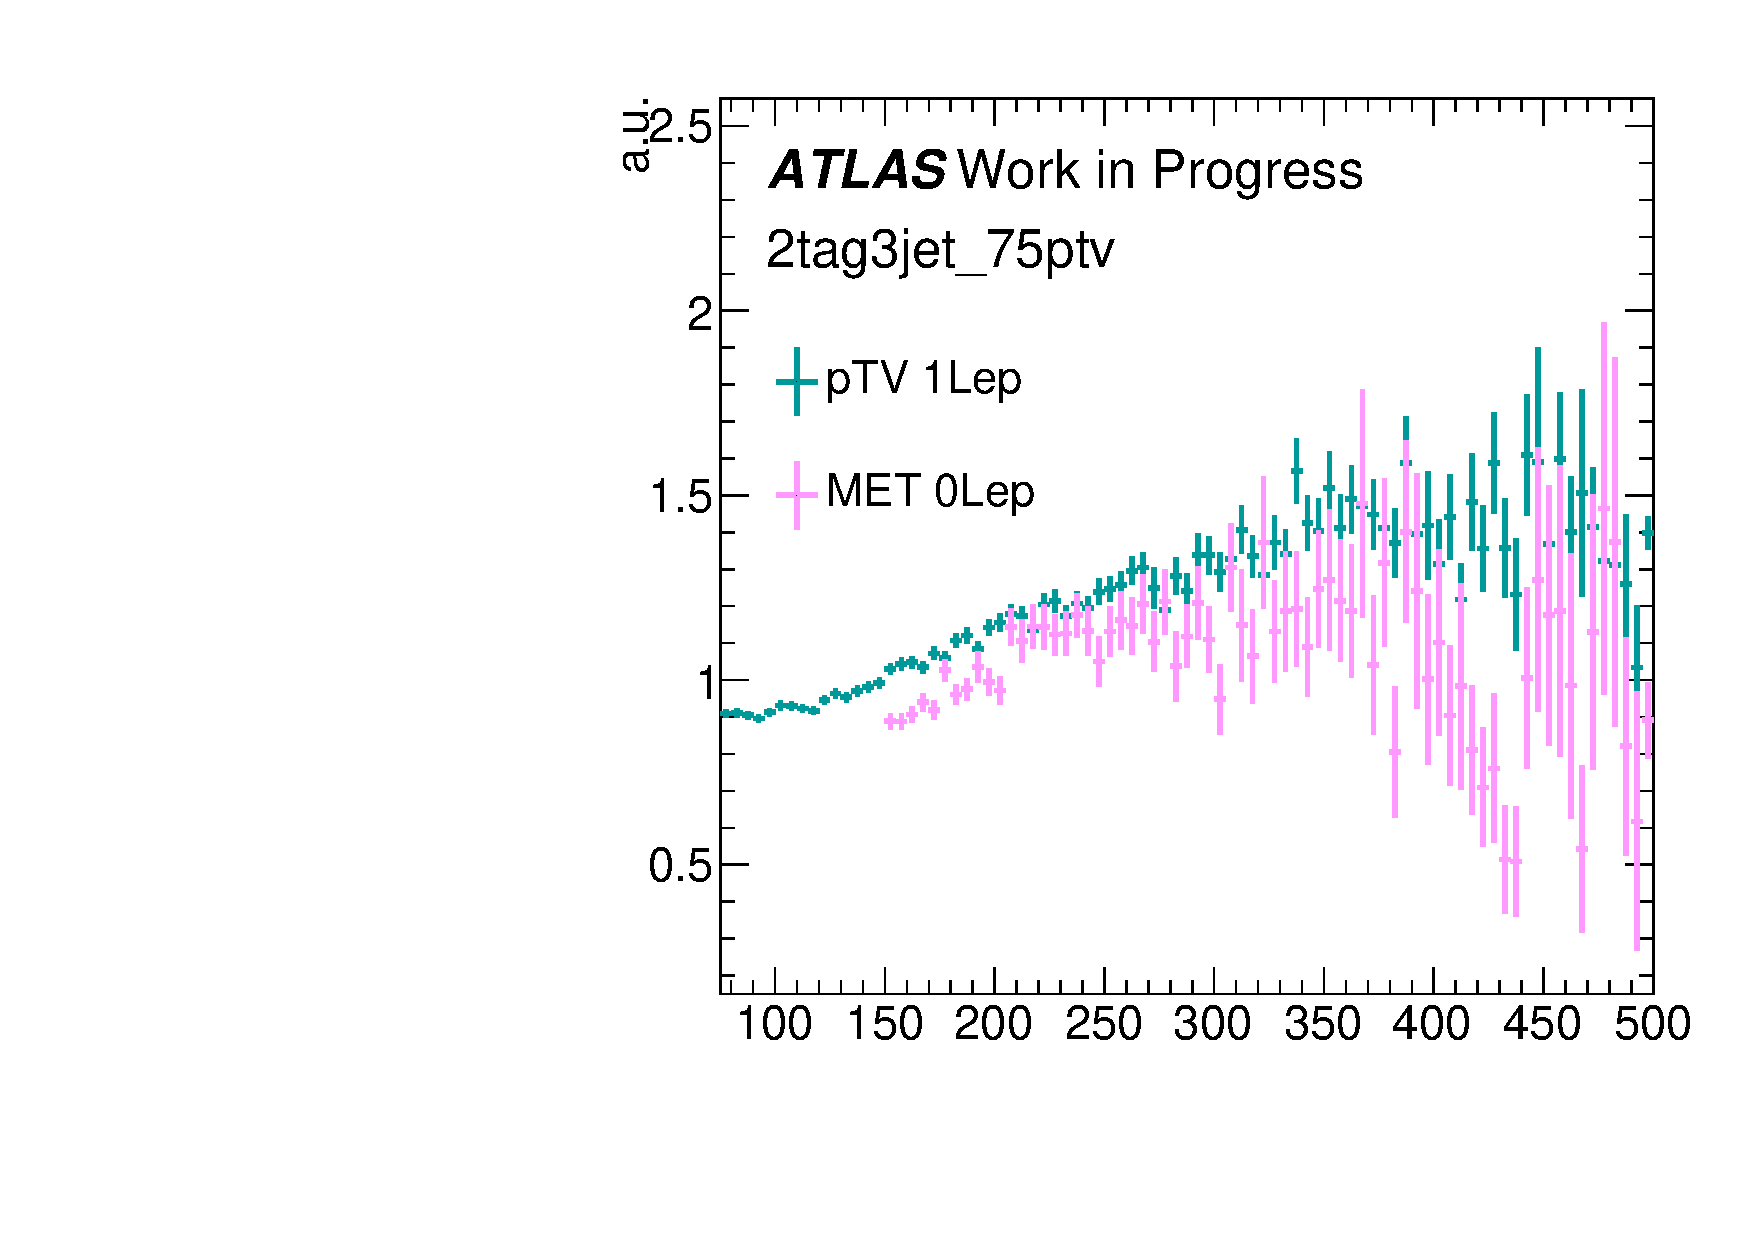
\includegraphics[width=0.45\textwidth]{01Lep_reweighting_shapes/ReweightingVarComparison_2tag3jet_75ptv_bl.pdf}
  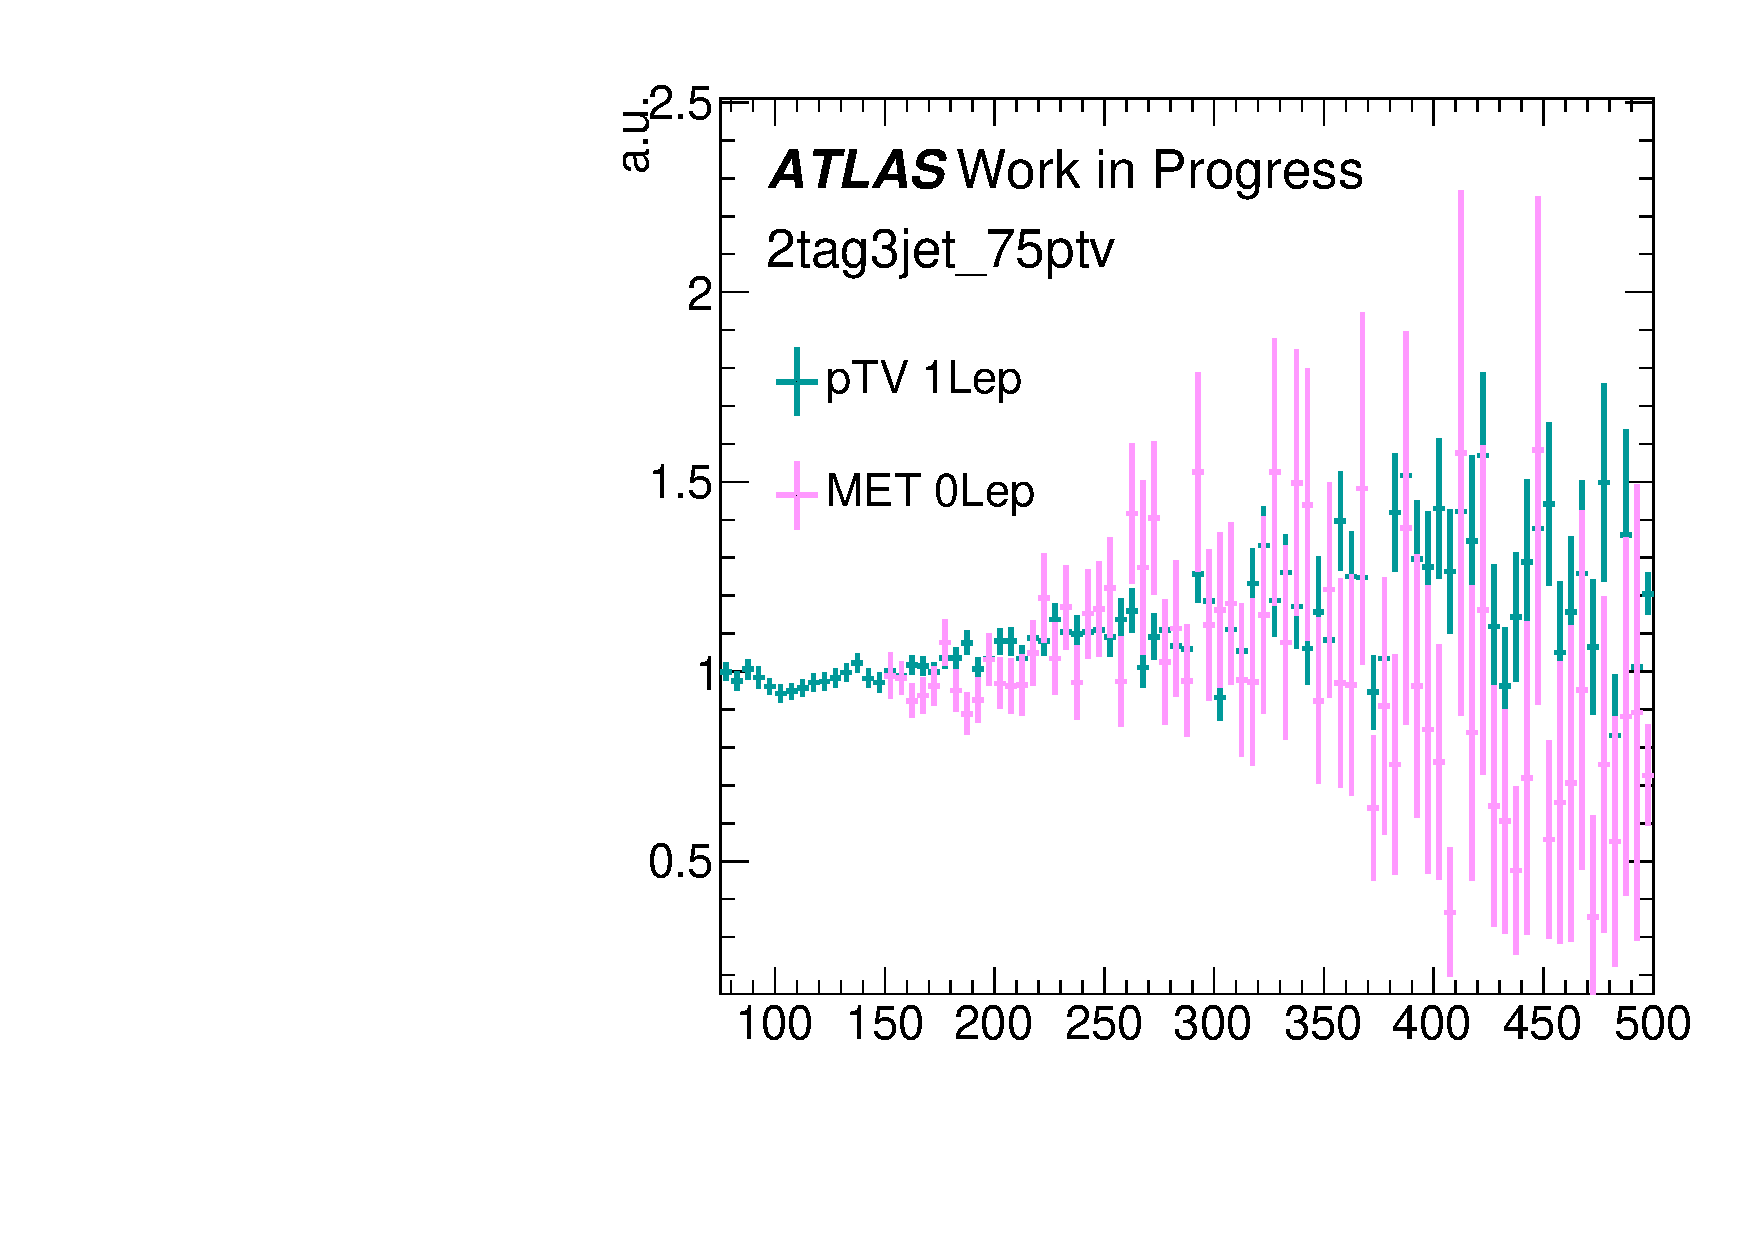
\includegraphics[width=0.45\textwidth]{01Lep_reweighting_shapes/ReweightingVarComparison_2tag3jet_75ptv_cc.pdf}
  \\
  \caption{$p_T^V$ and $E_T^{\text{miss}}$ shape systematics derived in the
    3--jet region of the 1-- and 0--lepton channels, respectively, for each
    heavy flavour sub-component.}
  \label{fig:wjets_01lep_3jet_SysWPtVBDTr}
\end{figure}

It can be seen the two shapes mostly agree within the statistical error which is
of course very large for the 0--lepton systematic. Furthermore
figure~\ref{fig:wjets_01lep_2jet_bl_SysWPtVBDTr_From150} shows  a comparison in
which both the $p_T^V$ and the $E_T^{\text{miss}}$ shapes in the 2--jet region
have been normalised to unit area in the $(p_T^V, E_T^{\text{miss}}) > 150$~\GeV\
range where it can be seen that agreement is event better further supporting the
validity of this choice.
\begin{figure}[ht!]
  \centering
  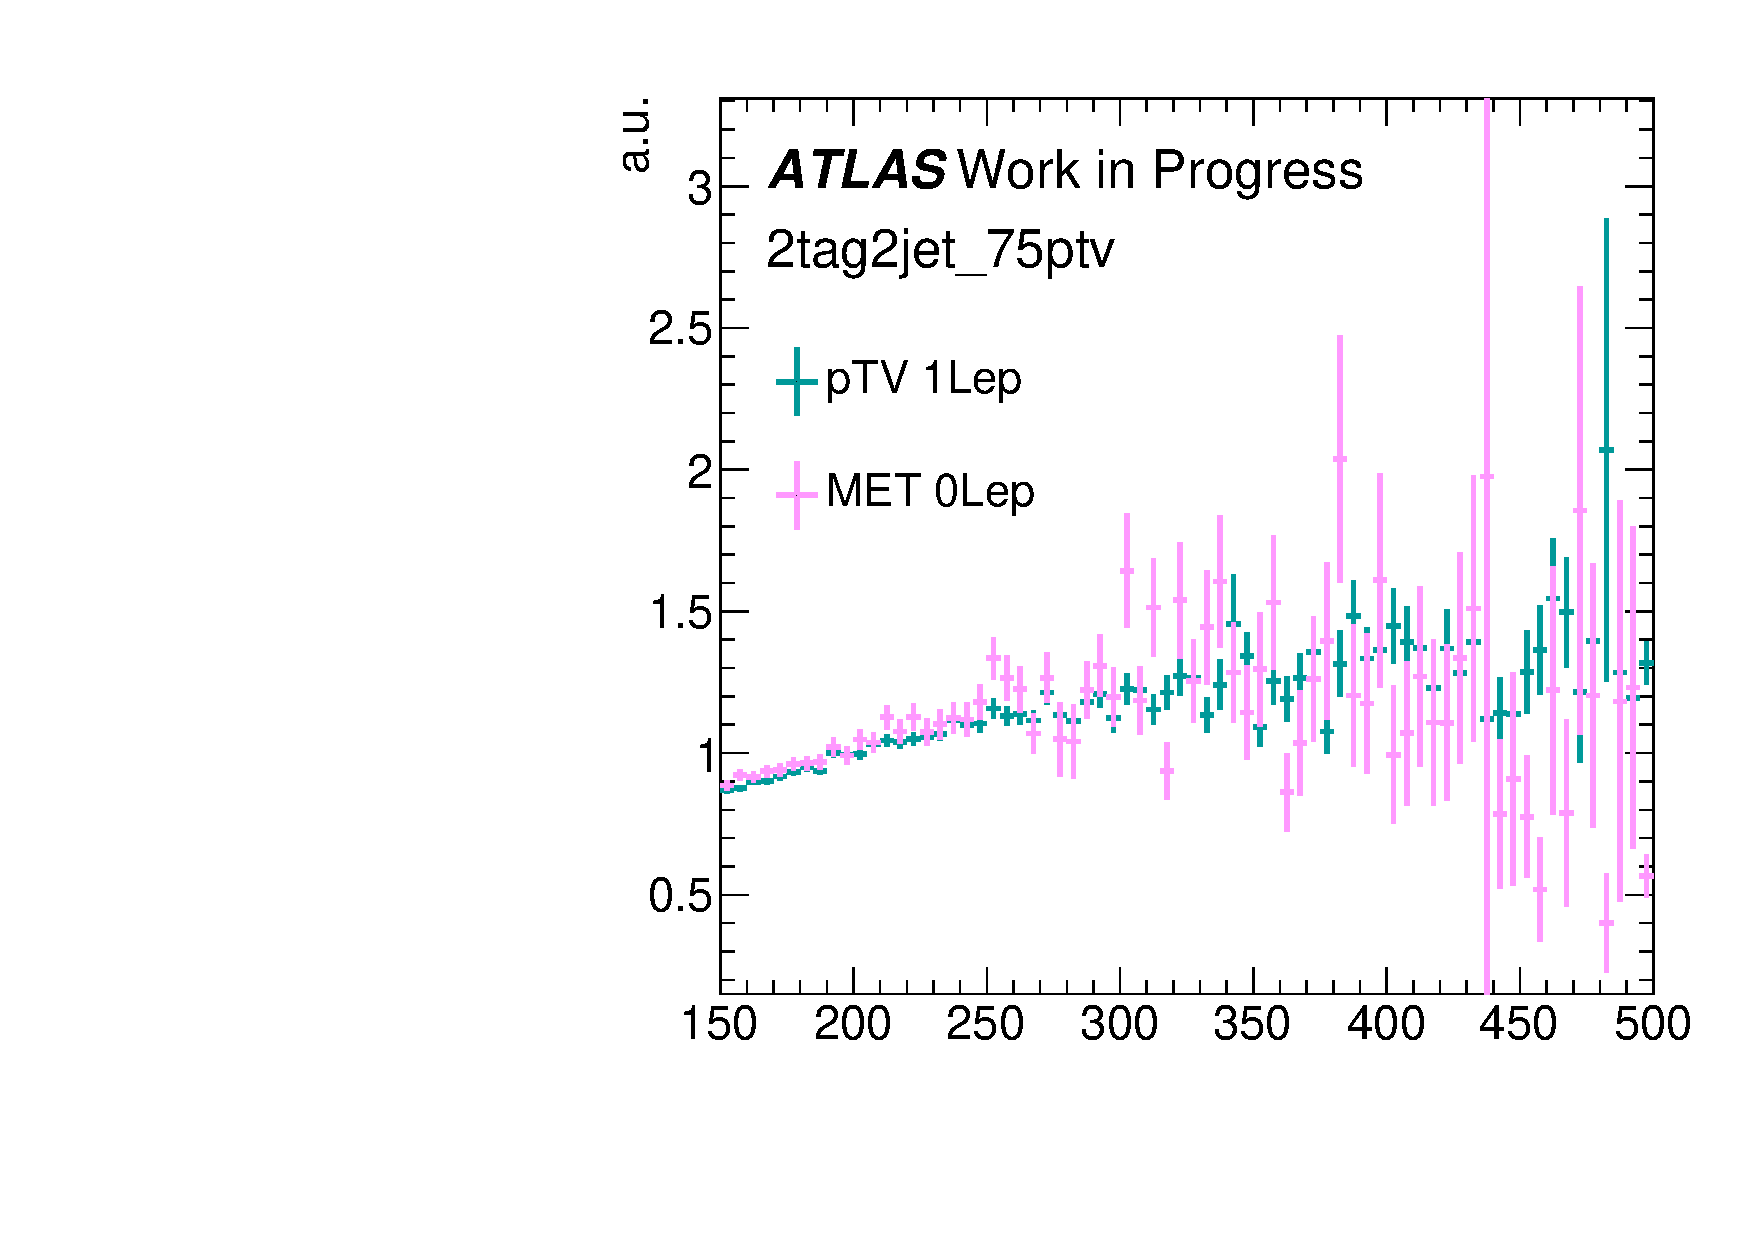
\includegraphics[width=0.45\textwidth]{01Lep_reweighting_shapes/ReweightingVarComparison_2tag2jet_75ptv_bl_NormalizedFrom150.pdf}
  \caption[A normalised comparison of 0-- and 1--lepton channel derived $p_T^V$ and
  $E_T^{\text{miss}}$ shape systematic uncertainties on $W+$jets
  events.]{$p_T^V$ and $E_T^{\text{miss}}$ shape systematic uncertainties
    derived in the 2--jet region of the 1-- and 0--lepton channels,
    respectively, for $W$+bl events, both normalized in the $p_T^V > 150$~\GeV
    and $E_T^{\text{miss}} > 150$~\GeV.}
  \label{fig:wjets_01lep_2jet_bl_SysWPtVBDTr_From150}
\end{figure}

As per the methodology of the factorised BDTr technique the nominal
\textsc{Sherpa}~2.2.1 events are re-weighted by the $p_T^V$ ratio with the
alternative prediction as was just discussed. The $p_T^V$ shape uncertainty is
therefore factorised out of the BDTr shape uncertainty. The re-weighted
\textsc{Sherpa}~2.2.1 events are then trained against the \textsc{MadGraph}
prediction in a BDT classifier that uses the input variables detailed in
table~\ref{tab:MVAinputs}. A separate training is performed in each jet category
and for each sub-component of the W + hf process in congruence with the 8
regions that the $p_T^V$ shape was derived in. Considering the output of the
classifier the ratio of the scores of the nominal and alternative predictions
enter into the profile-likelihood fit as a nuisance parameter called
\texttt{SysBDTr\_W\_SHtoMG5}. All of the following plots shown contain only W +
bb events as this is the dominant and most important component of the W + hf
process and indeed the W + jets background in the analysis.

In order to check the validity of the method the re-weighted nominal predictions
of key inputs to the analyisis MVA are plotted against the nominal and
alternative predictions in figures~\ref{fig:wjets_1lep_2jet_BDTrClosure_1}
and~\ref{fig:wjets_0lep_2jet_BDTrClosure_1} for the 1-- and 0--lepton channels
respectively in the 2--jet category.
\begin{figure}[ht!]
  \centering
  \includegraphics[width=0.45\textwidth]{1Lep_BDTbased_closure/1lepton_2tag2jet_75ptv_SR+CR_pTV_bb.pdf}
  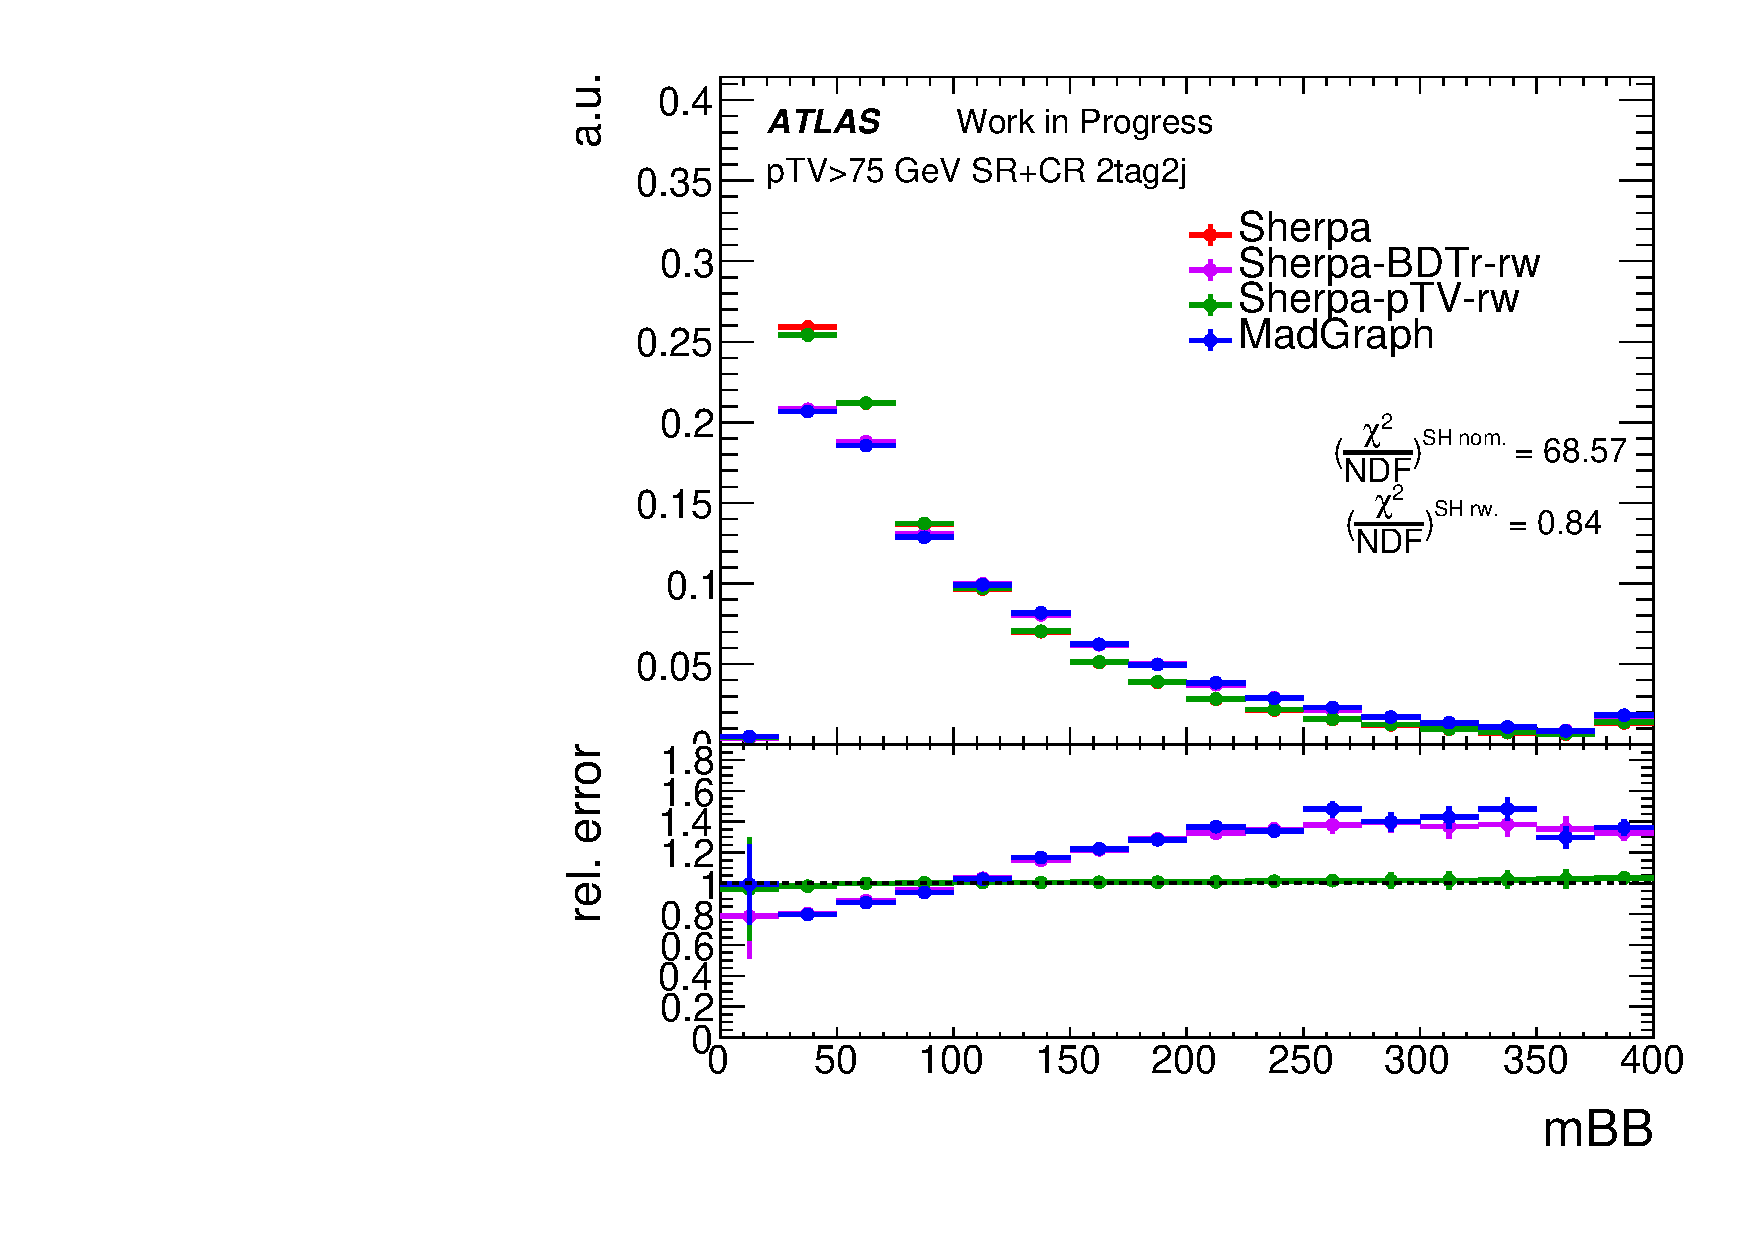
\includegraphics[width=0.45\textwidth]{1Lep_BDTbased_closure/1lepton_2tag2jet_75ptv_SR+CR_mBB_bb.pdf}  \\
  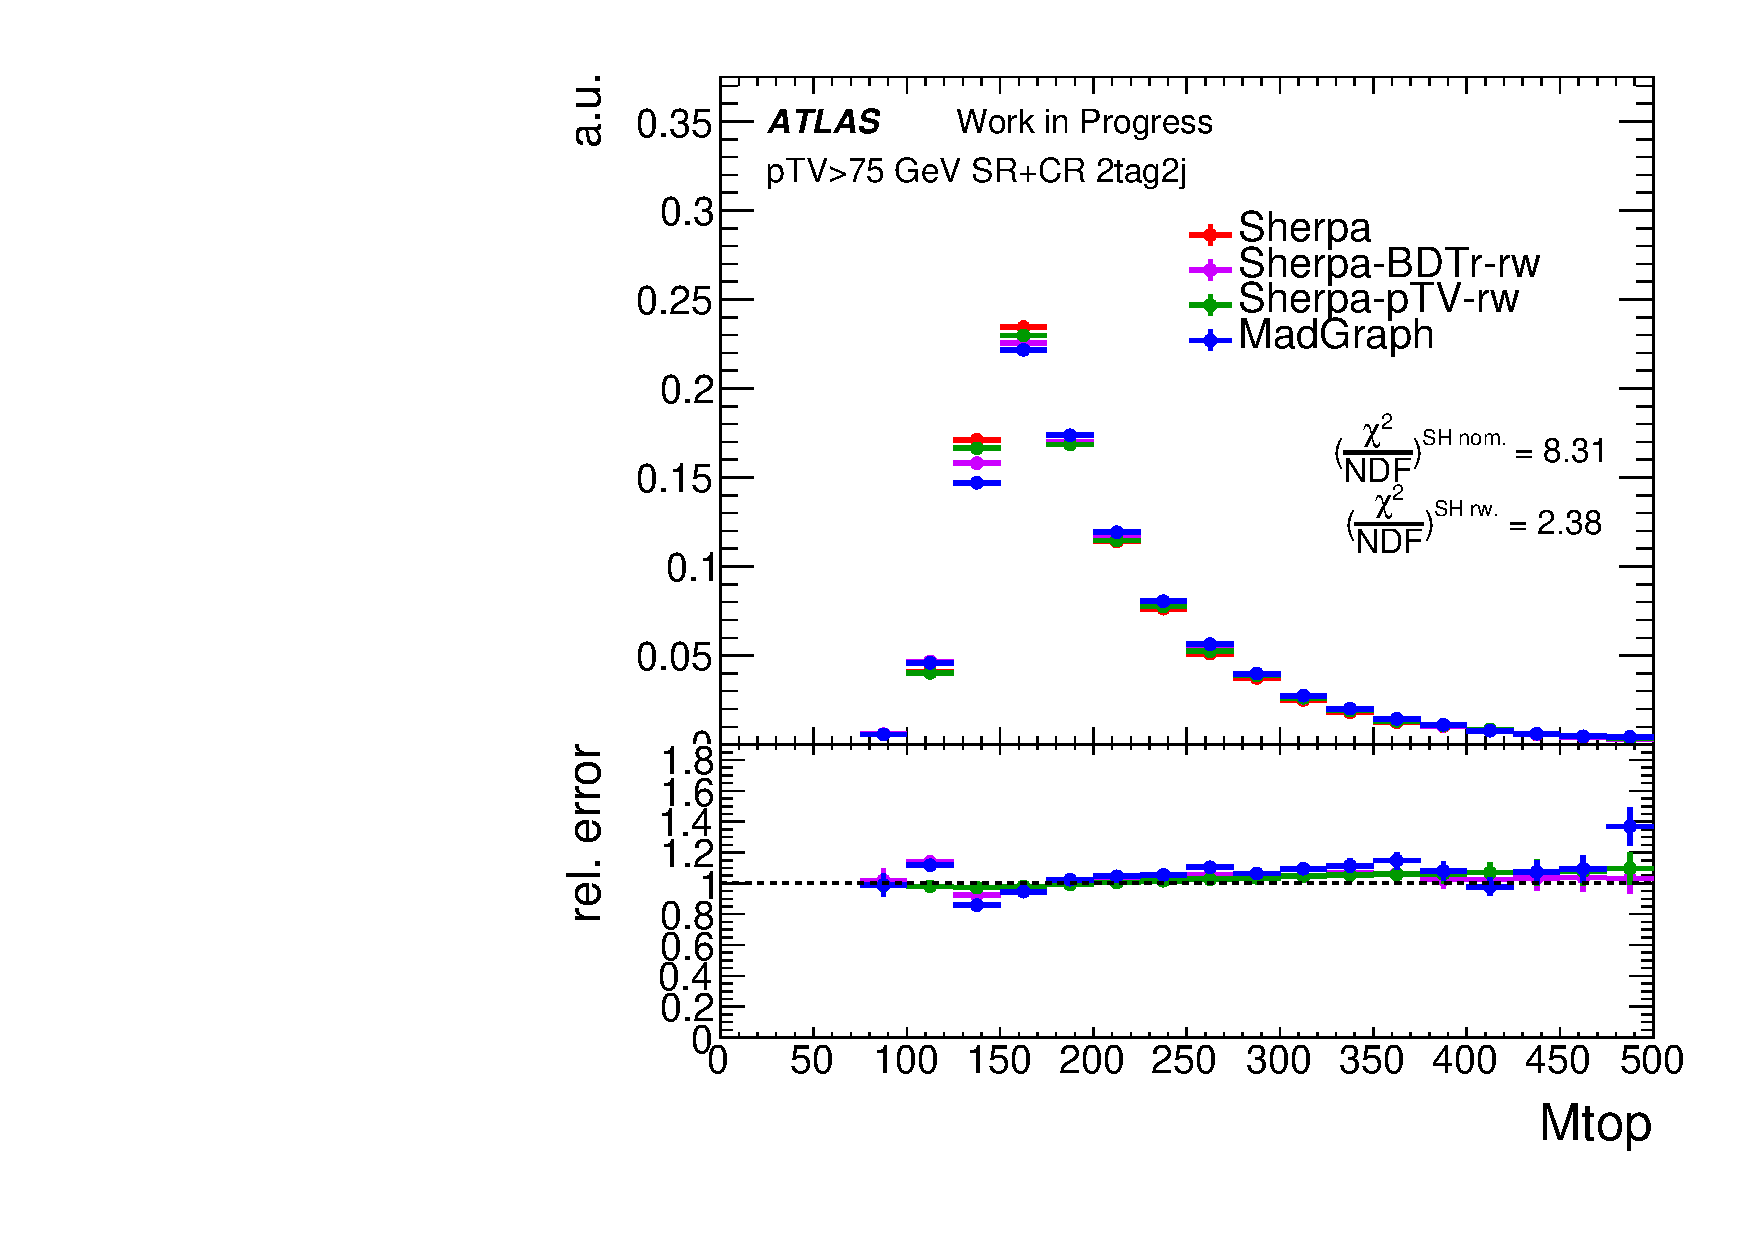
\includegraphics[width=0.45\textwidth]{1Lep_BDTbased_closure/1lepton_2tag2jet_75ptv_SR+CR_Mtop_bb.pdf}
  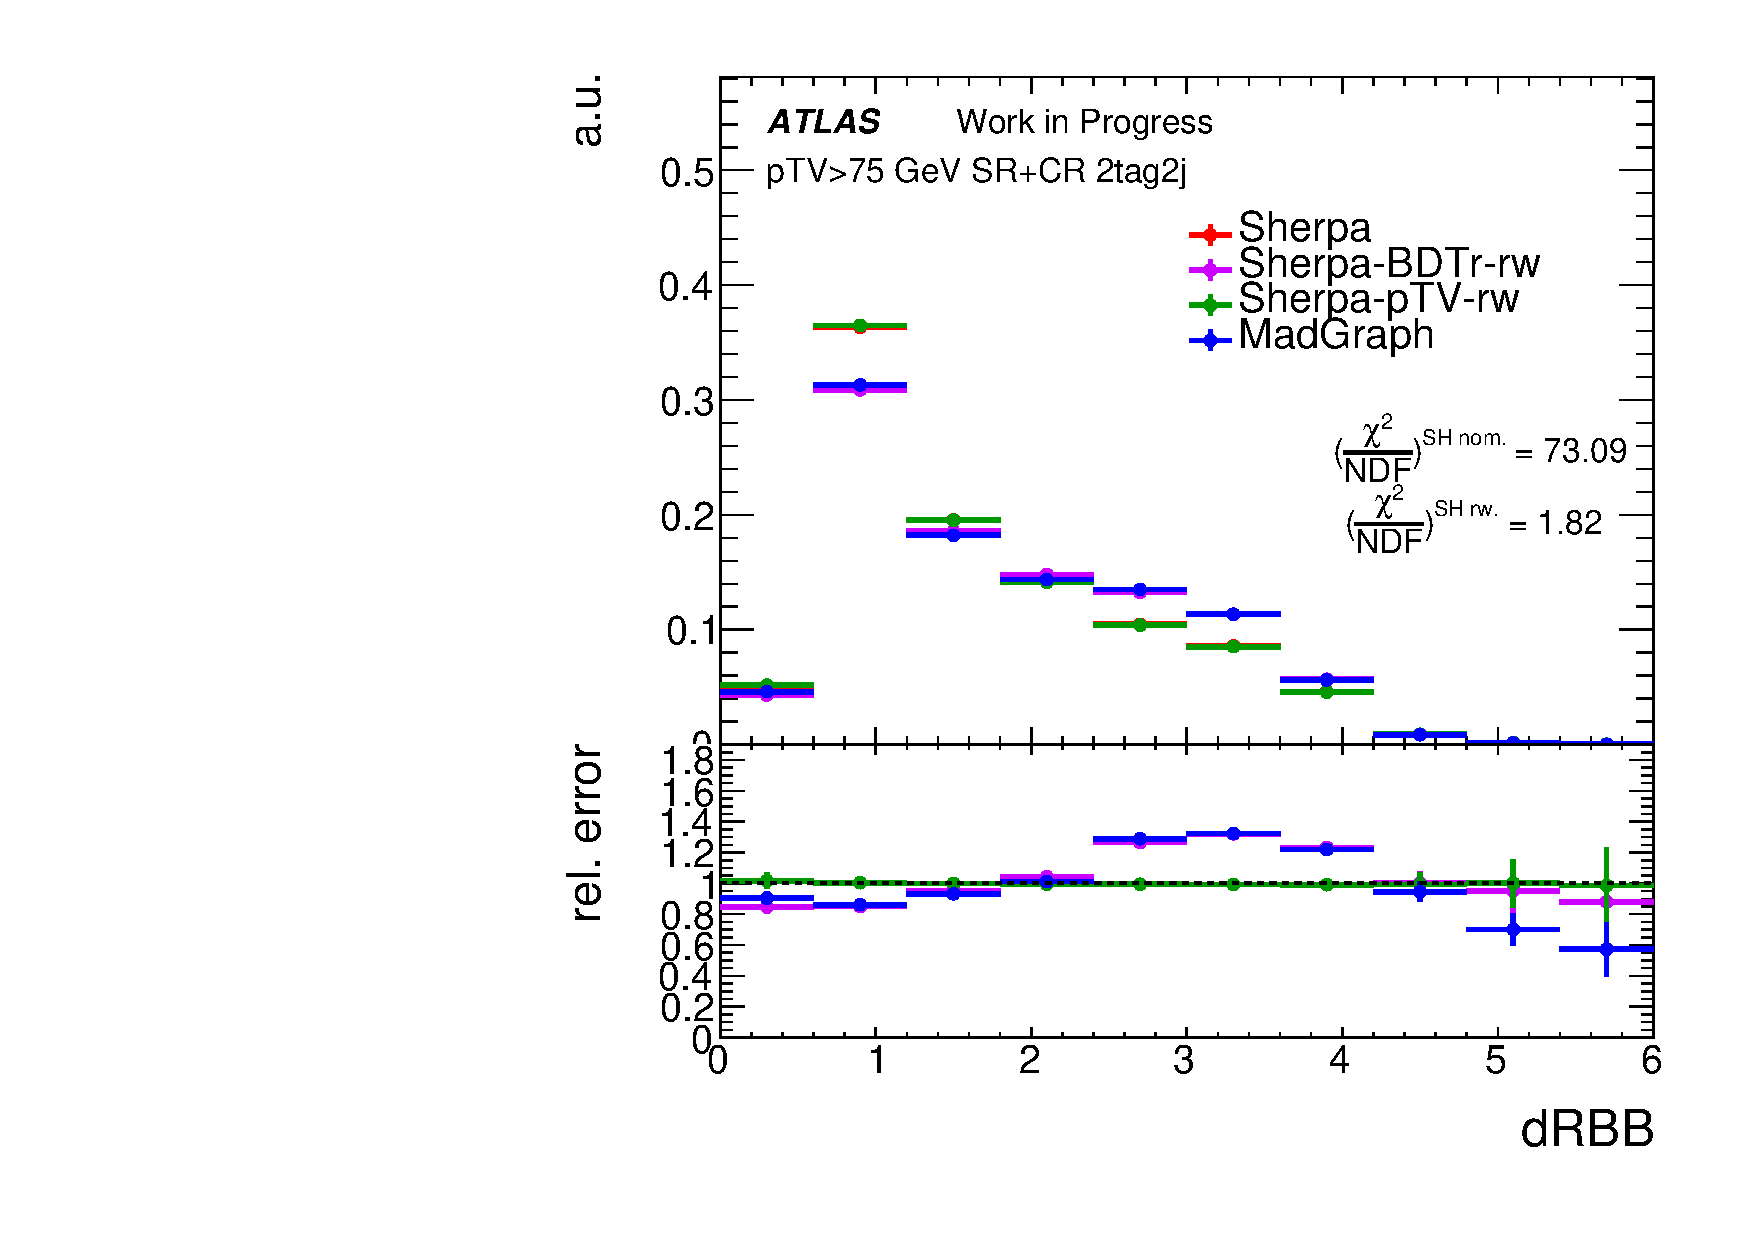
\includegraphics[width=0.45\textwidth]{1Lep_BDTbased_closure/1lepton_2tag2jet_75ptv_SR+CR_dRBB_bb.pdf} \\
  \caption{Histograms of the nominal predictions in the 1--lepton 2--jet region
    of variables entering into the analysis MVA are shown alongside the
    alternative predictions from \textsc{MadGraph} and the re-weighted nominal
    prediction. The $p_T^V$ shape systematic which was calculated in advance of
    the training is shown in green.}
  \label{fig:wjets_1lep_2jet_BDTrClosure_1}
\end{figure}
\begin{figure}[H]
  \centering
  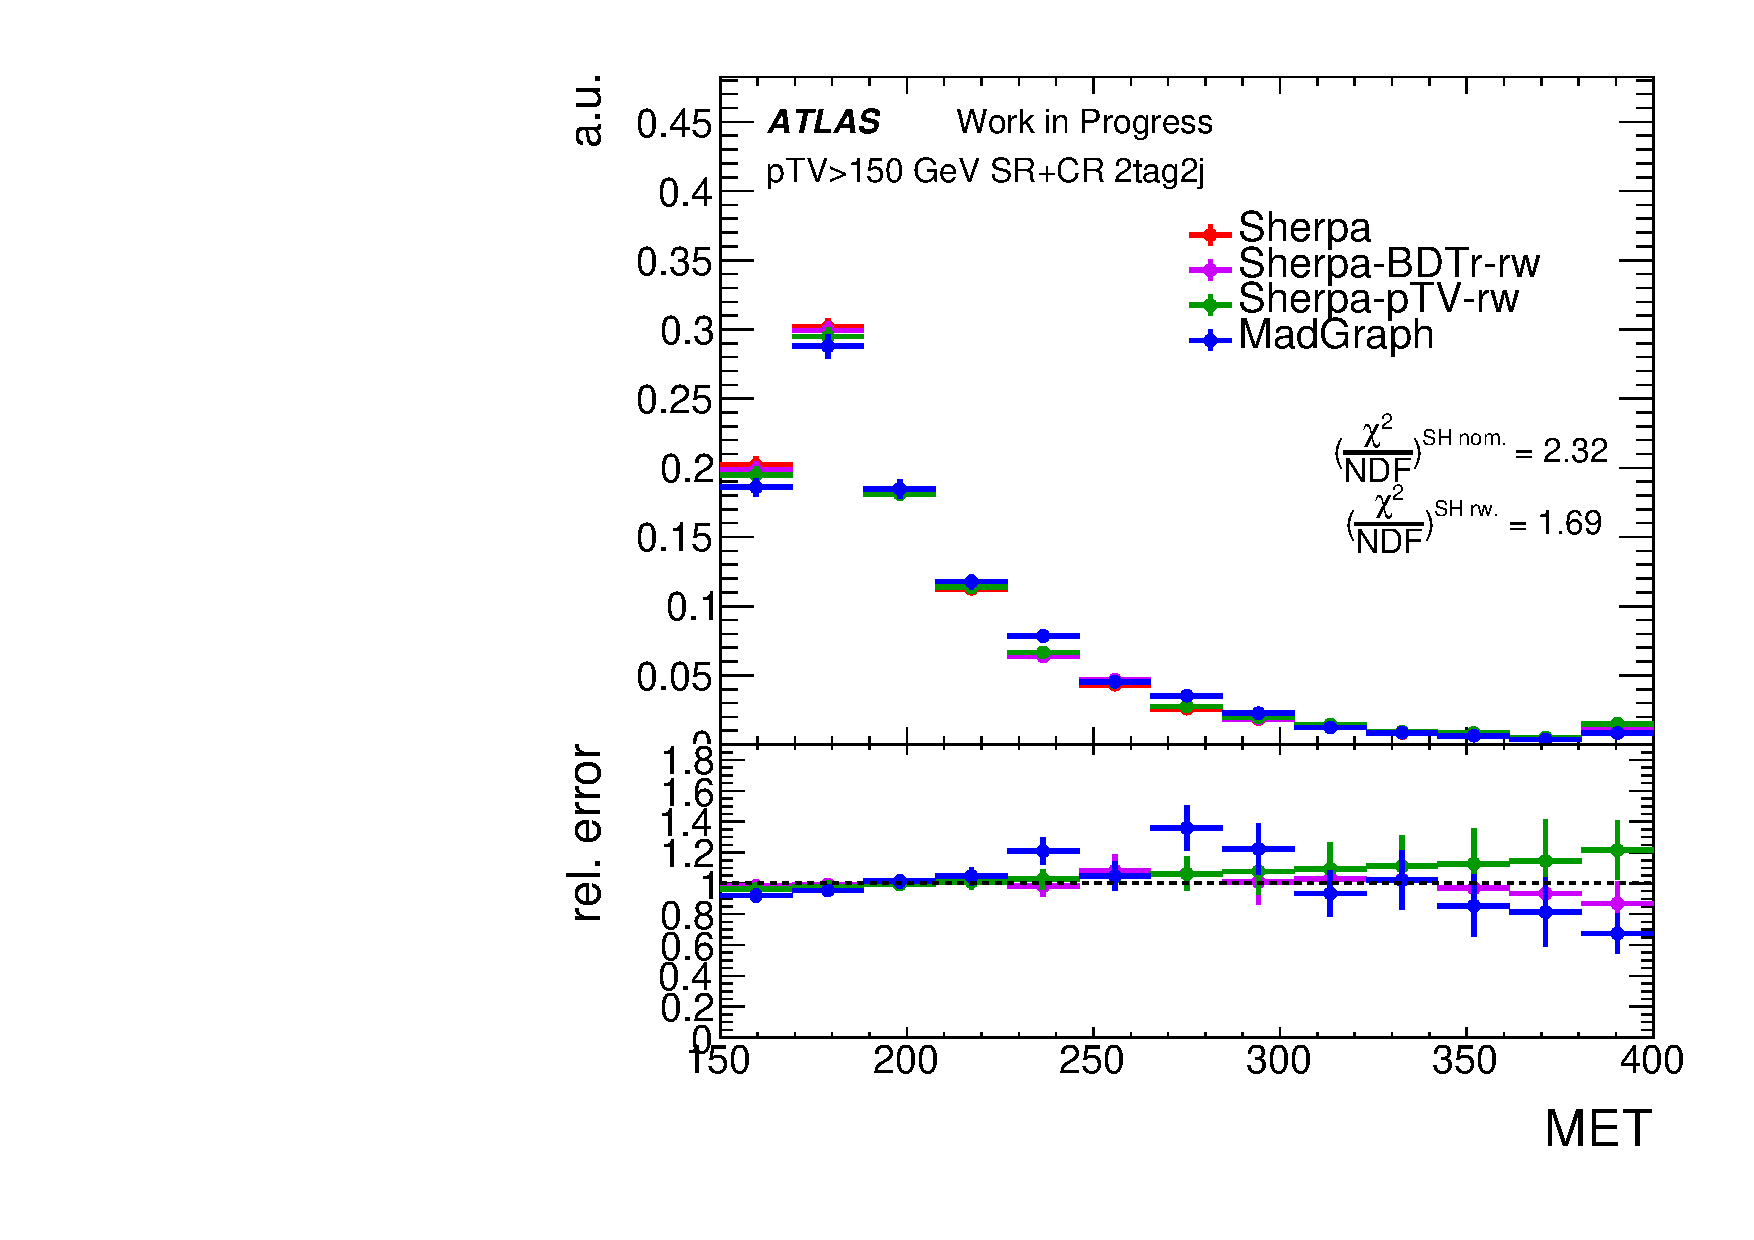
\includegraphics[width=0.45\textwidth]{0Lep_BDTbased_closure/0lepton_2tag2jet_150ptv_SR+CR_MET_bb.pdf}
  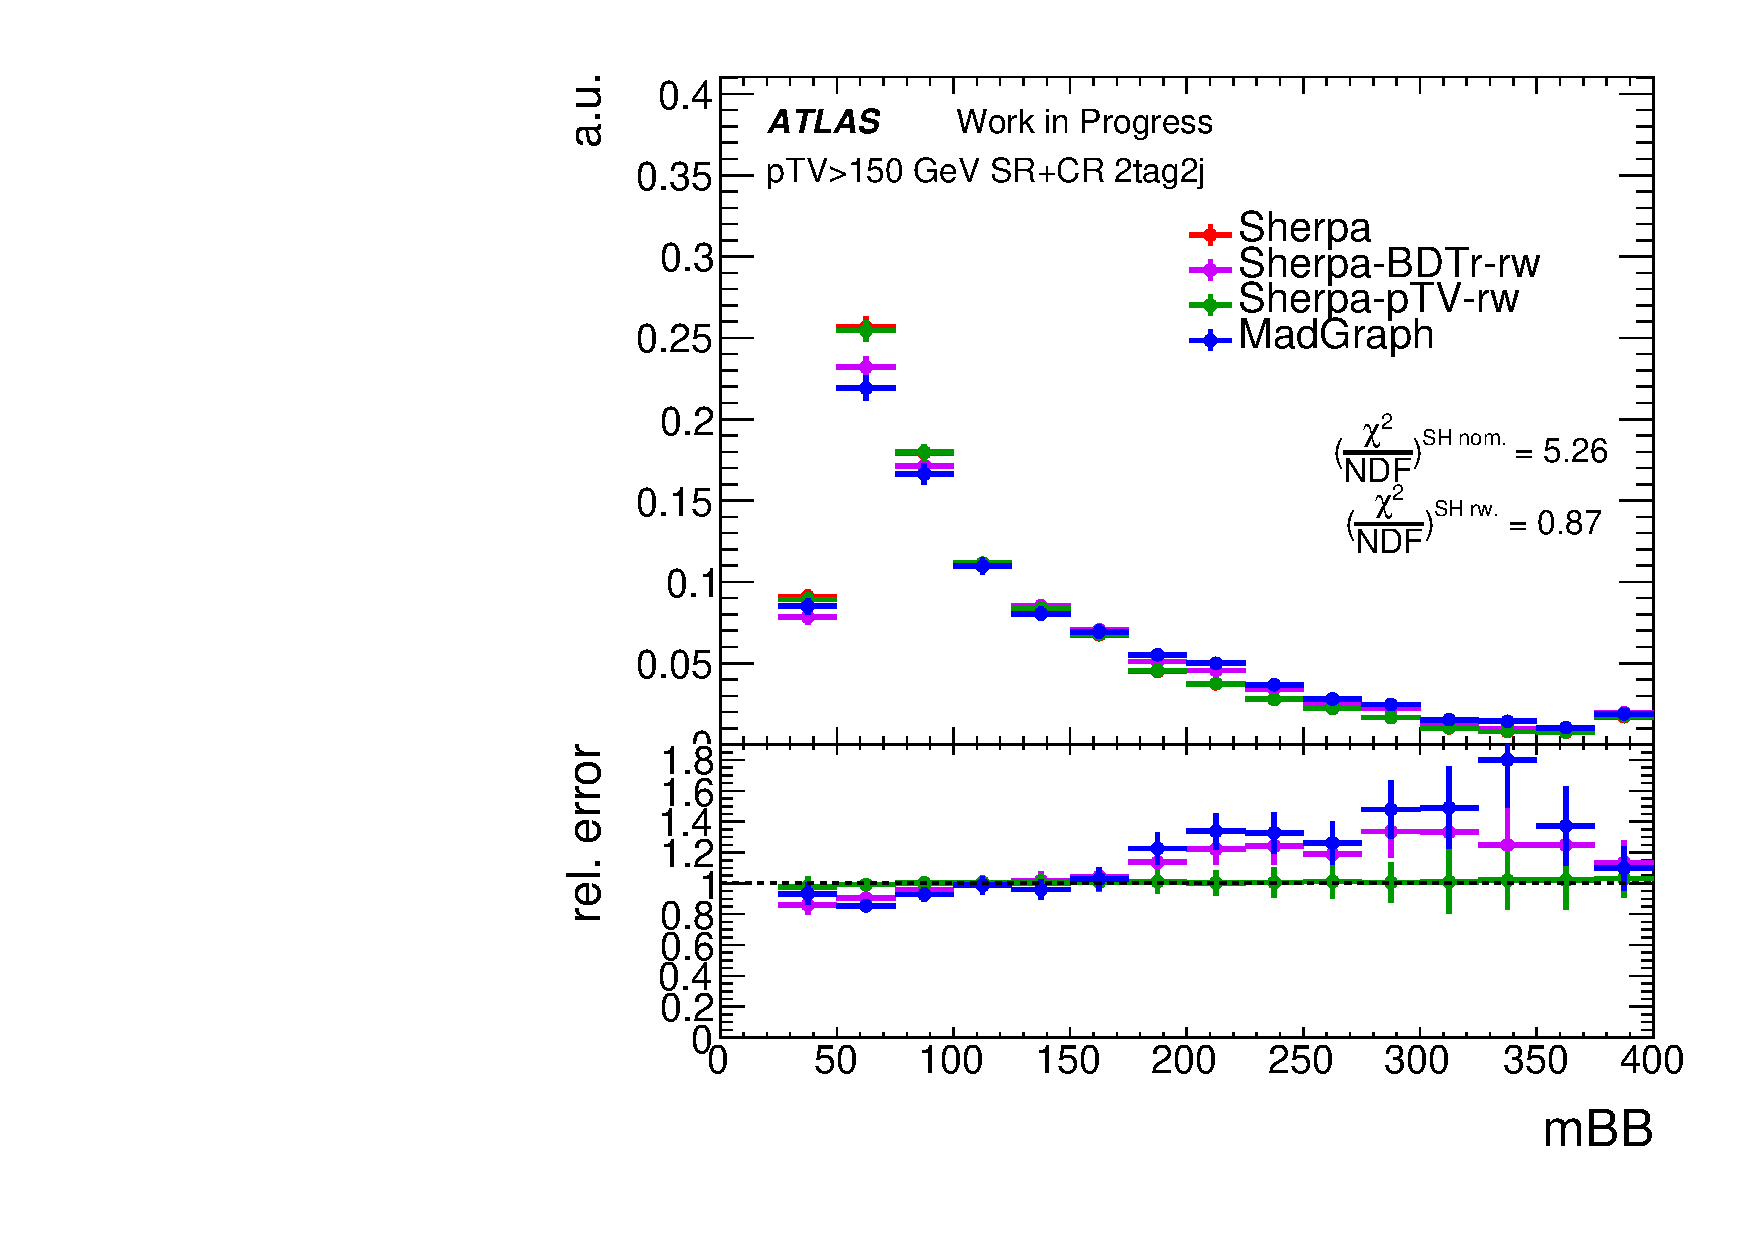
\includegraphics[width=0.45\textwidth]{0Lep_BDTbased_closure/0lepton_2tag2jet_150ptv_SR+CR_mBB_bb.pdf}  \\
  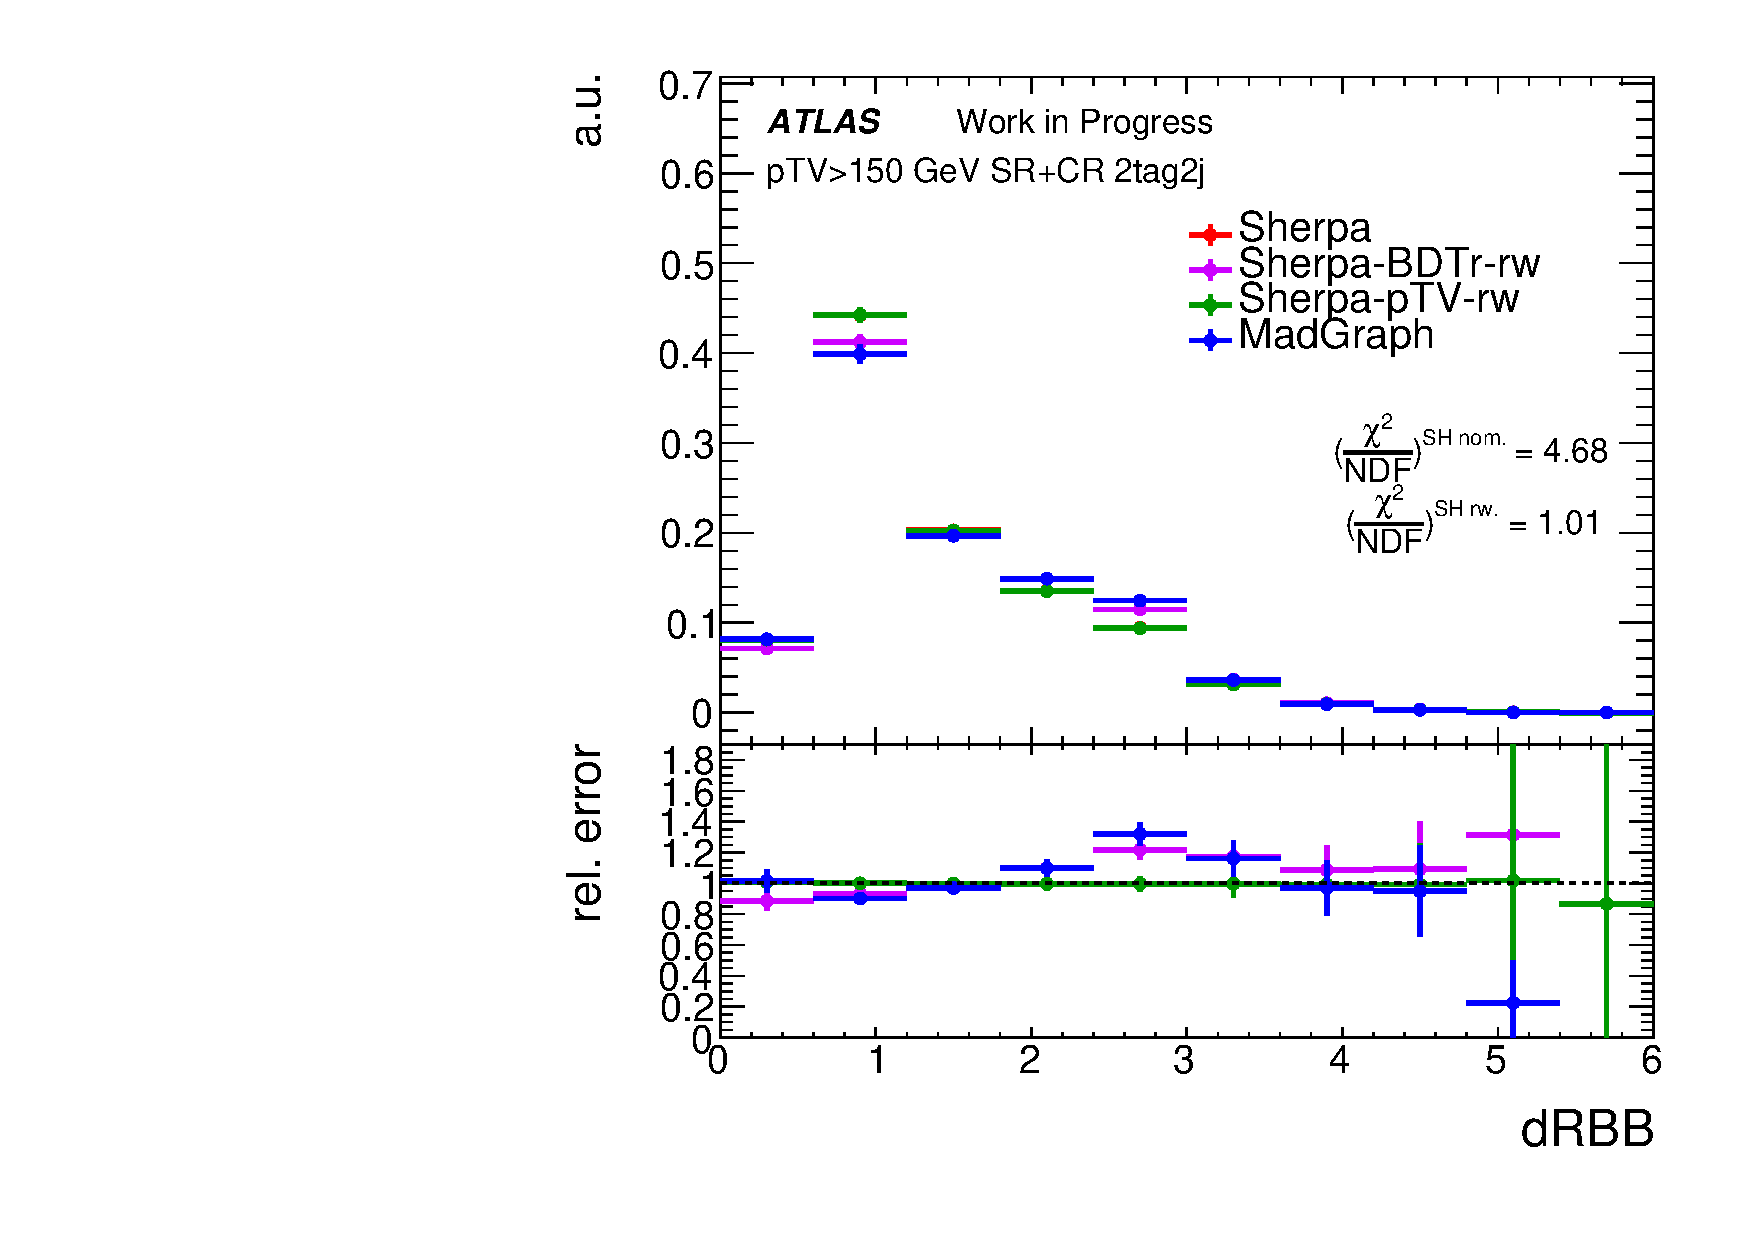
\includegraphics[width=0.45\textwidth]{0Lep_BDTbased_closure/0lepton_2tag2jet_150ptv_SR+CR_dRBB_bb.pdf}
  \\
  \caption{Histograms of the nominal predictions in the 0--lepton 2--jet region
    of variables entering into the analysis MVA are shown alongside the
    alternative predictions from \textsc{MadGraph} and the re-weighted nominal
    prediction. The $p_T^V$ shape systematic which was calculated in advance of
    the training is shown in green.}
    \label{fig:wjets_0lep_2jet_BDTrClosure_1}
\end{figure}
Should the re-weighted nominal inputs match
the shapes of the alternative inputs then the method is considered to be valid.
Indeed upon inspection one can see that this is largely the case across the
board apart from small levels of disagreement. These small levels of
disagreement are disregarded as the two most important variables in the
determination of the analysis BDT score, $m(b, \bar{b})$, $p_T^V$ and
$E_T^{\text{miss}}$ have good levels of agreement.

The actual effect of the factorised BDTr systematic uncertainty on the analysis
BDT score is shown in figures~\ref{fig:wjets_1lep_FullRun2MVA_BDTrClosure}
and~\ref{fig:wjets_0lep_FullRun2MVA_BDTrClosure} for the 1-- and 0--lepton
channels respectively. 
\begin{figure}[ht!]
  \centering
  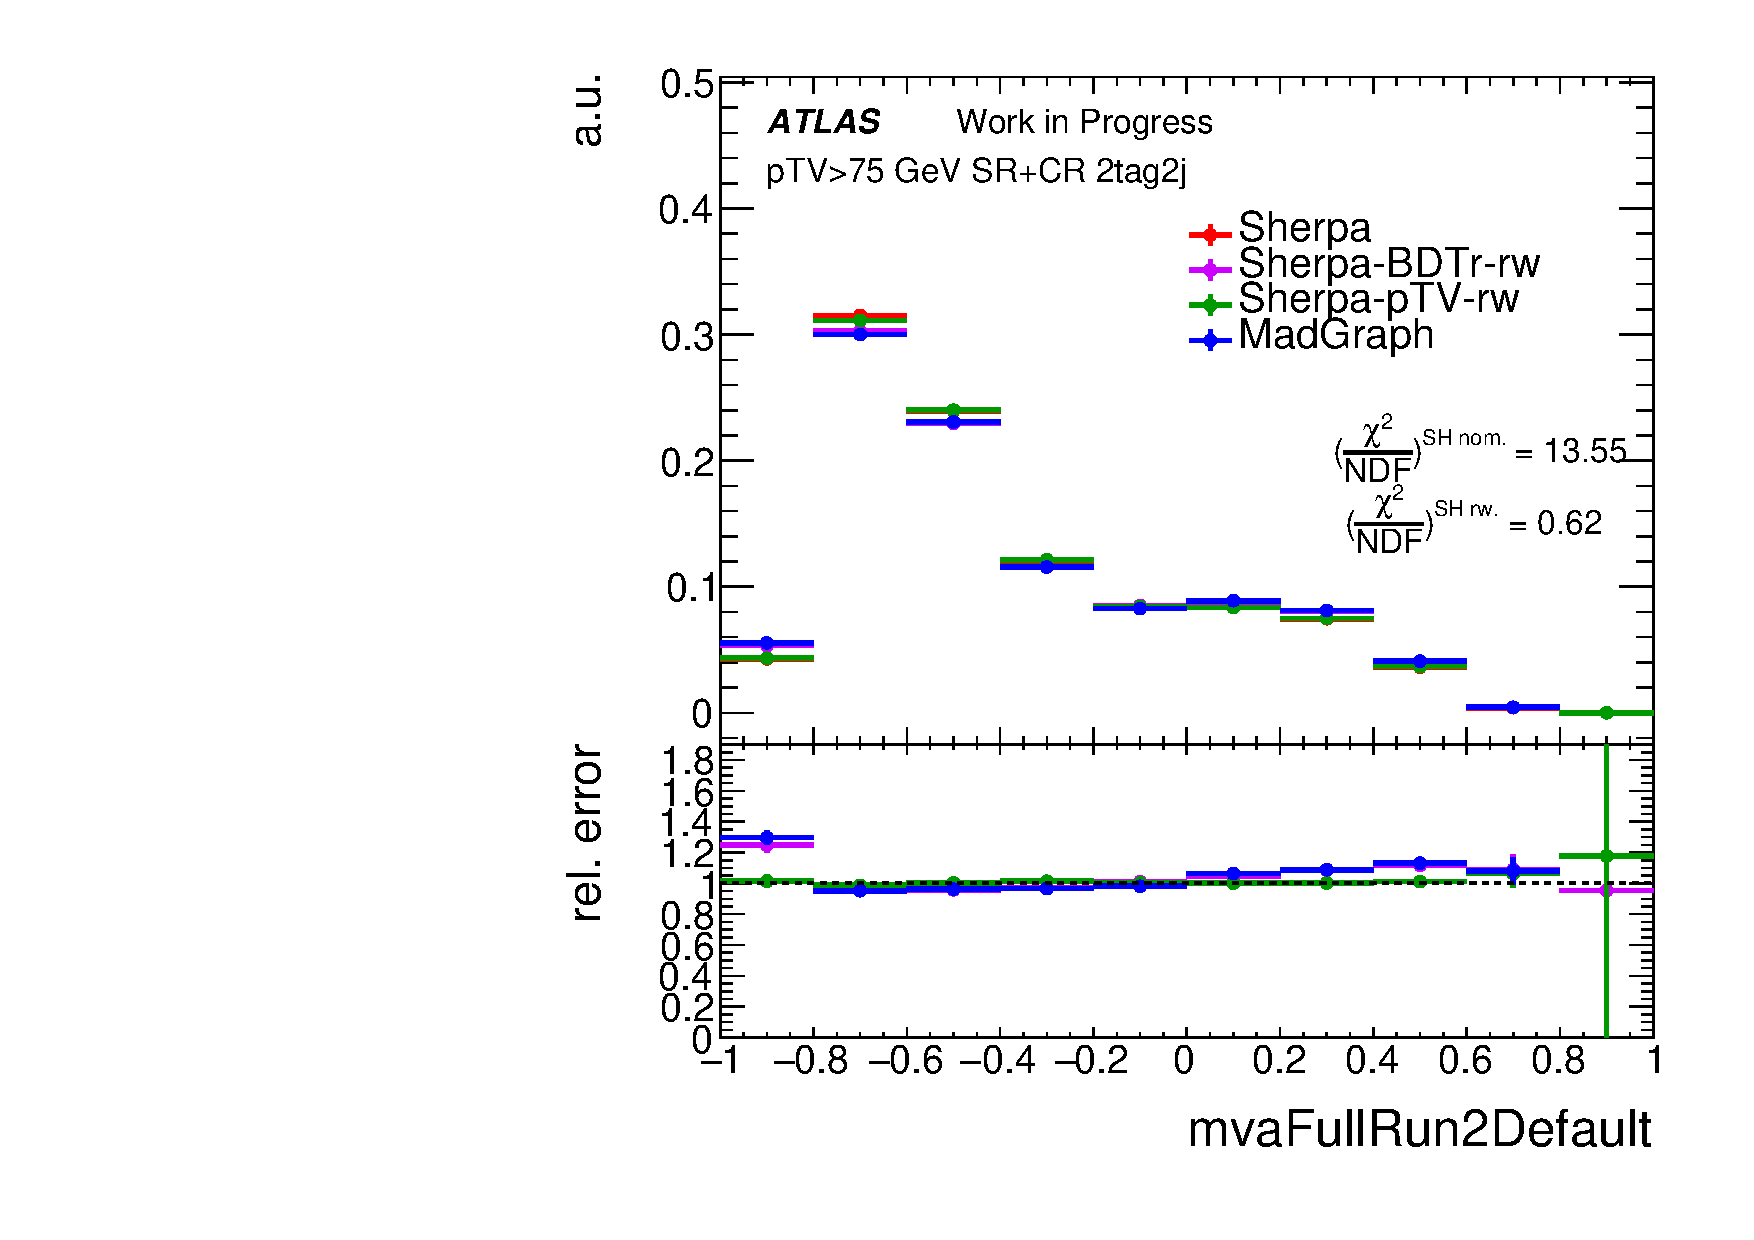
\includegraphics[width=0.45\textwidth]{1Lep_BDTbased_closure/1lepton_2tag2jet_75ptv_SR+CR_mvaFullRun2Default_bb.pdf}
  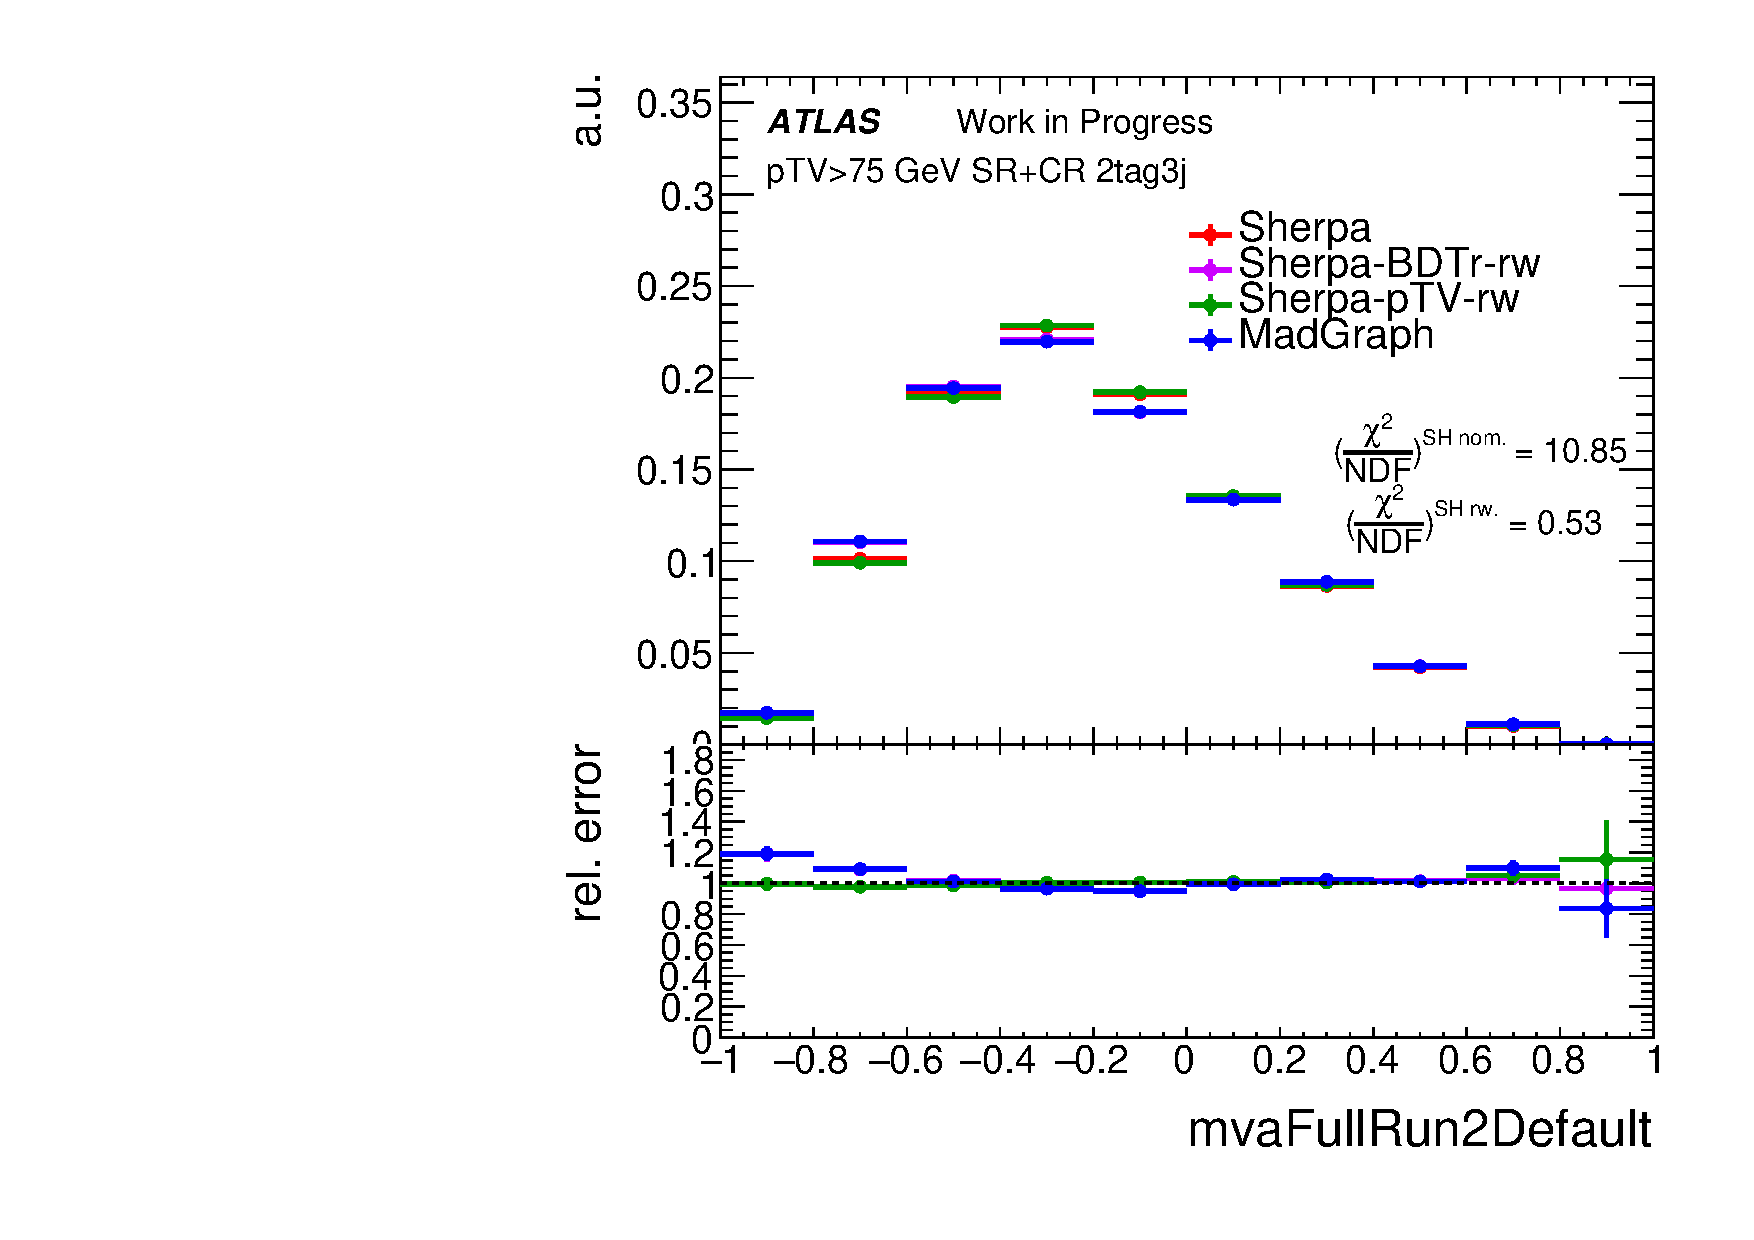
\includegraphics[width=0.45\textwidth]{1Lep_BDTbased_closure/1lepton_2tag3jet_75ptv_SR+CR_mvaFullRun2Default_bb.pdf}  \\
  \caption[Nominal, alternative and re-weighted nominal predictions of $W+$jets
  events (1--lepton channel, MVA score).]{Histograms of the nominal predictions
    in the 1--lepton channel of the analysis MVA score are shown alongside the
    alternative predictions from \textsc{MadGraph} and the re-weighted nominal
    prediction. The $p_{\mathrm{T}}^V$ shape systematic which was calculated in advance of
    the training is shown in green. Only W + bb events are shown.}
    \label{fig:wjets_1lep_FullRun2MVA_BDTrClosure}
\end{figure}
\begin{figure}[ht!]
  \centering
  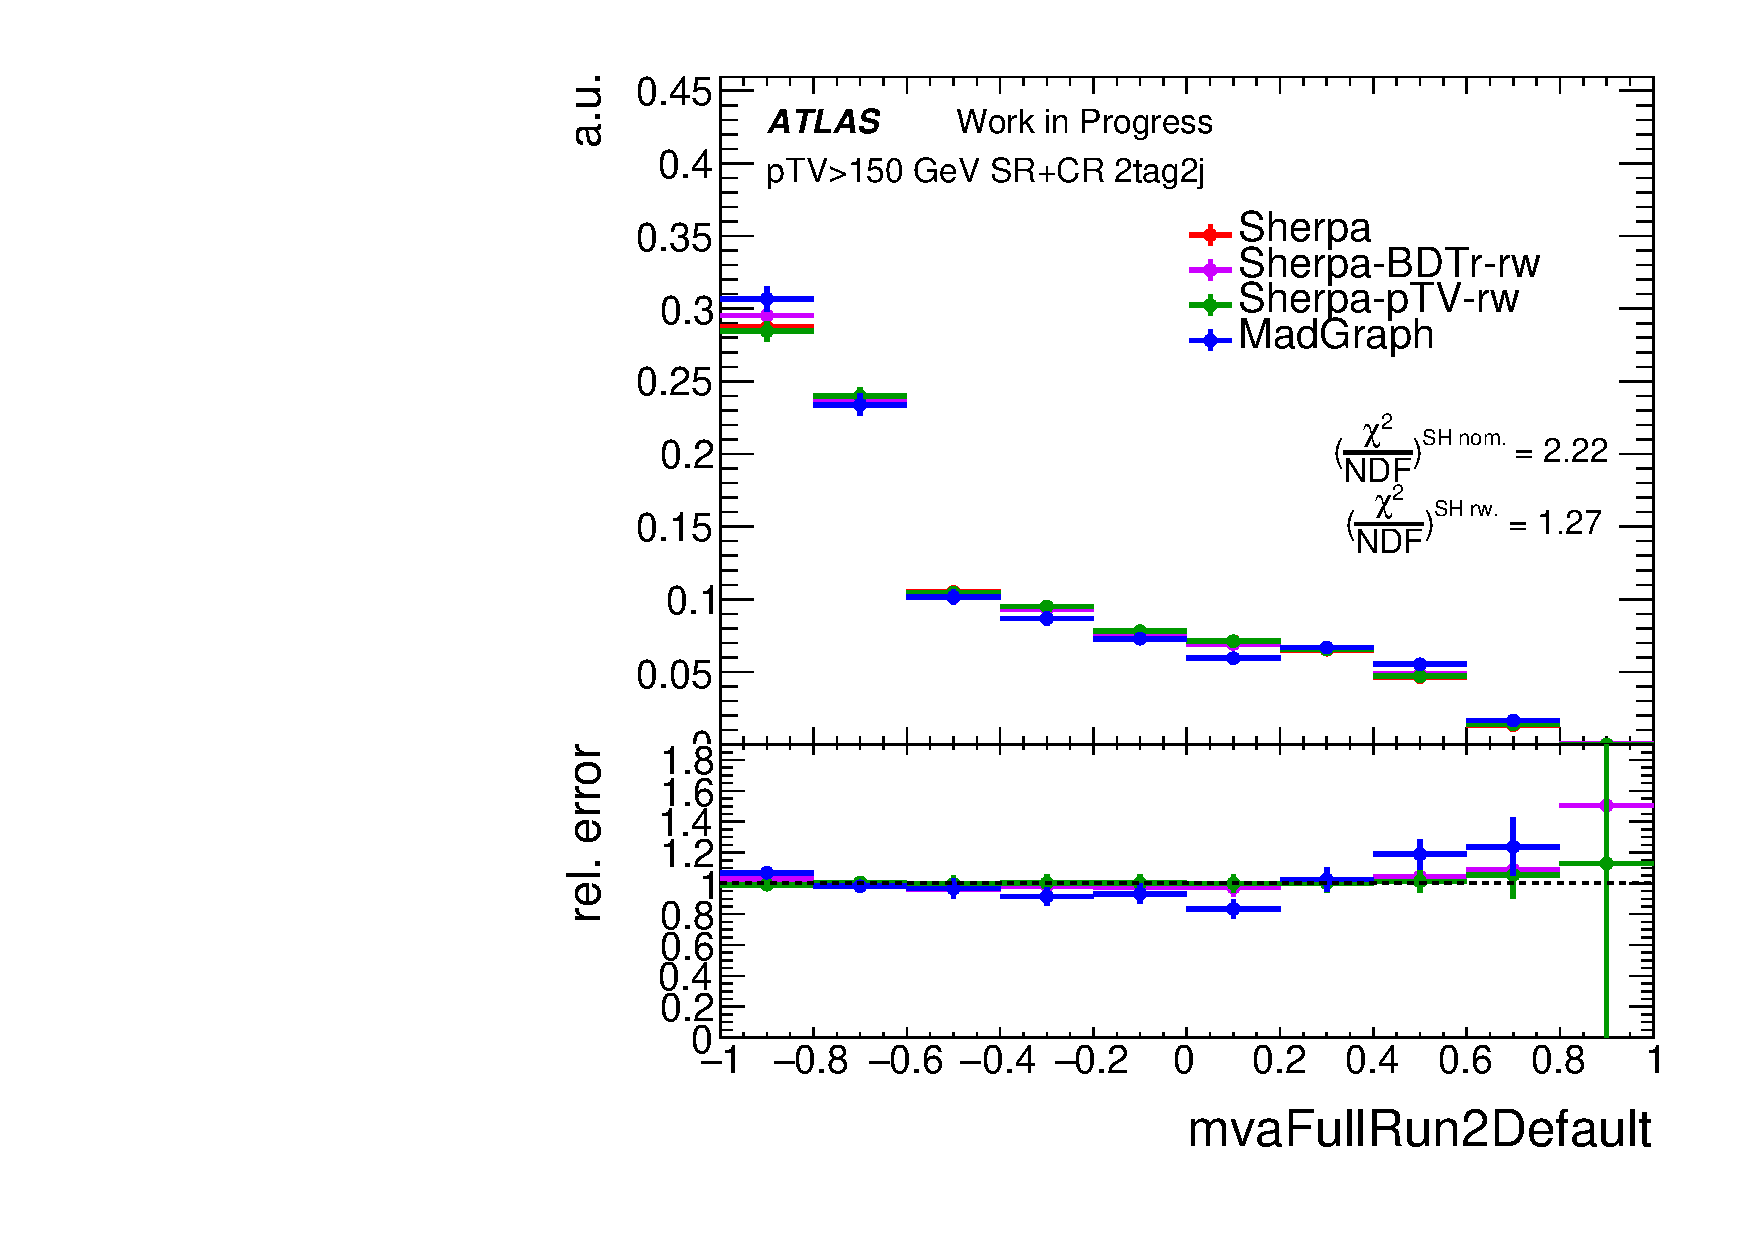
\includegraphics[width=0.45\textwidth]{0Lep_BDTbased_closure/0lepton_2tag2jet_150ptv_SR+CR_mvaFullRun2Default_bb.pdf}
  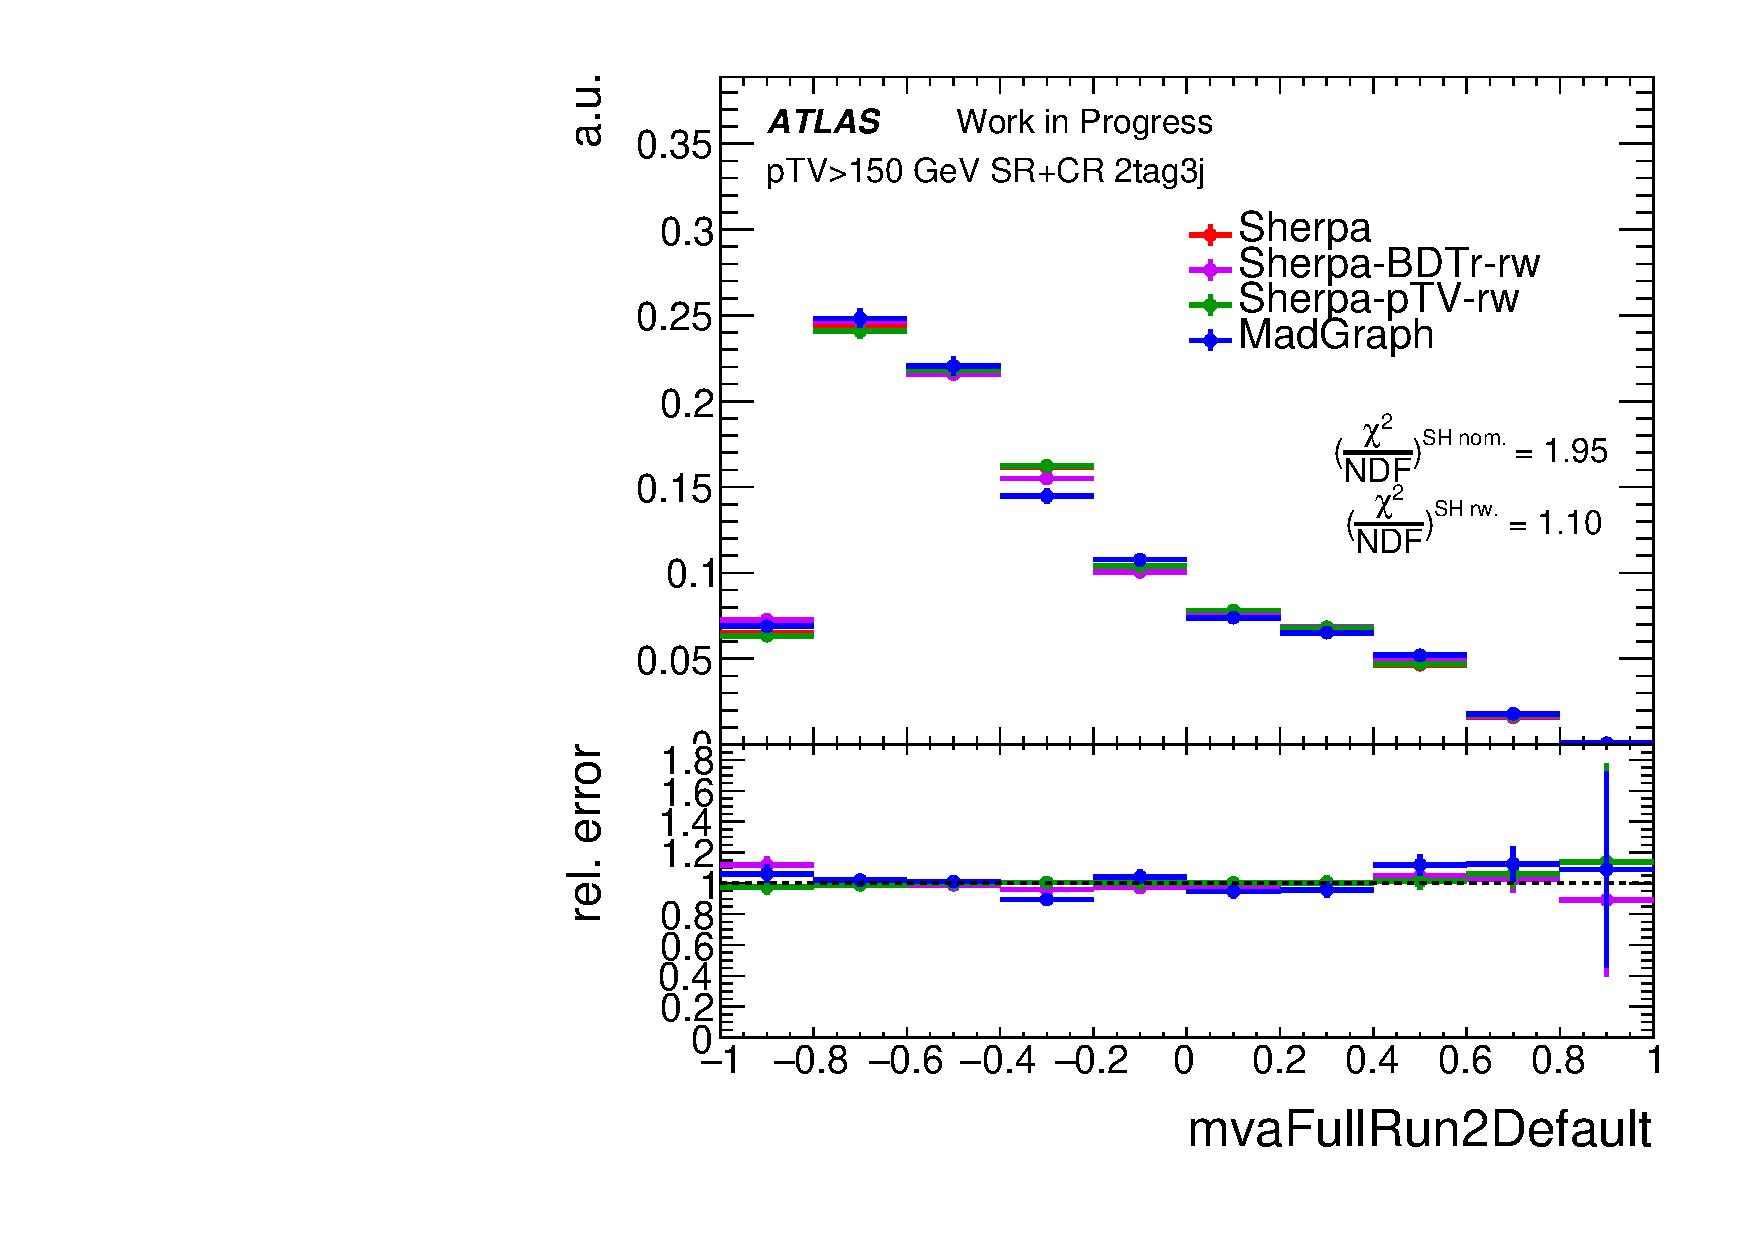
\includegraphics[width=0.45\textwidth]{0Lep_BDTbased_closure/0lepton_2tag3jet_150ptv_SR+CR_mvaFullRun2Default_bb.pdf}
  \\
  \caption[Nominal, alternative and re-weighted nominal predictions of W + jets
  events (0--lepton channel, MVA score).]{Histograms
    of the nominal predictions in the 0--lepton channel of the analysis MVA
    score are shown alongside the alternative predictions from \textsc{MadGraph}
    and the re-weighted nominal prediction. The $p_T^V$ shape systematic which
    was calculated in advance of the training is shown in green. Only W + bb
    events are shown.}
  \label{fig:wjets_0lep_FullRun2MVA_BDTrClosure}
\end{figure}
Tables~\ref{tab:wjets-extrapolation_uncertainties_pTV}
and~\ref{tab:wjets-extrapolation_uncertainties_BDTr} in the appendix show the
extrapolation uncertainties induced by the $p_T^V$ and factorised BDTr shape
systematic uncertainties respectively.
\clearpage
\newpage

\subsection{Systematic Uncertainties on Z + jets Events}
\label{sec:zjets-systs}

Systematic uncertainties are considered in the 0-- and 2--lepton channels only
as there is a negligible contribution of this background in the 1--lepton channel.

\subsubsection{Normalisation and Acceptance Uncertainties}

Several normalisation and acceptance uncertainties are considered for the Z +
jets background, they are summarised in table~\ref{tab:zjetsnorm}.
\begin{table}[!htpb] 
  \centering
  \resizebox{\textwidth}{!}{%
    \begin{tabular}{ l l S[table-format=3.2] S[table-format=3.2] S[table-format=3.2] S[table-format=3.2] S[table-format=3.2] S[table-format=3.2] } 
      \toprule
      &  & \multicolumn{3}{c}{\bfseries 2--jet} & \multicolumn{3}{ c }{\bfseries ($\bm{\geq$})3--jets} \\ 
      {\bfseries Name} & {\bfseries Process} & {\bfseries CR$_{\text{low}}$}  & {\bfseries CR$_{\text{high}}$} & {\bfseries SR} & {\bfseries CR$_{\text{low}}$}  &  {\bfseries CR$_{\text{high}}$} & {\bfseries SR} \\ 
      \midrule
      {\bfseries 0--lepton} & & & & & & & \\
      \texttt{SysZclNorm}            & $Z$+l    &   \multicolumn{6}{c}{23\% } \\
      \texttt{SysZlNorm}             & $Z$+cl   &   \multicolumn{6}{c}{ 18\% } \\
      \texttt{norm\_Zbb\_J2}       & $Z$+hf   &  \multicolumn{3}{c}{ Floating Normalisation} &  \multicolumn{3}{ c }{ N/A } \\
      \texttt{norm\_Zbb\_J3}       & $Z$+hf   &  \multicolumn{3}{c}{ N/A } &  \multicolumn{3}{ c }{ Floating Normalisation} \\
      \texttt{SysZbbNorm\_0L}    	  & $Z$+hf  & \multicolumn{6}{c}{7\%} \\
      \texttt{SysZbbPTV}           & $Z$+hf   &    \multicolumn{6}{ c }{$p^{V}_{\mathrm{T}}$ dependent migrations covered by $p^{V}_{\mathrm{T}}$ shape systematic}       \\
      \texttt{SysZbbCRSRExtrapolation\_CRLow} & $Z+$hf & -6.0\% & N/A & N/A & -6.6\% & N/A & N/A \\
      \texttt{SysZbbCRSRExtrapolation\_CRHigh} & $Z+$hf & N/A & 3.8\% & N/A & N/A & 3.9\% & N/A \\ 
      {\bfseries 2--lepton} & & & & & & & \\
      \texttt{SysZclNorm}    & $Z$+l  & \multicolumn{6}{c}{23\% } \\
      \texttt{SysZlNorm}     & $Z$+cl &   \multicolumn{6}{c}{ 18\% } \\
      \texttt{norm\_Zbb\_J2} & $Z$+hf &  \multicolumn{3}{c}{ Floating Normalisation} &  \multicolumn{3}{ c }{ N/A } \\
      \texttt{norm\_Zbb\_J3} & $Z$+hf &  \multicolumn{3}{c}{ N/A } &  \multicolumn{3}{ c }{ Floating Normalisation} \\
      \texttt{SysZbbPTV}     & $Z$+hf &    \multicolumn{6}{c}{$p^{V}_{\mathrm{T}}$ dependent migrations covered by $p^{V}_{\mathrm{T}}$ shape systematic}       \\
      \texttt{SysZbbCRSRExtrapolation\_CRLow} & $Z+$hf $p_{\mathrm{T}}^V > 150$~\GeV   &  -9.9\% & N/A & N/A & -3.8\% & N/A & N/A \\
      \texttt{SysZbbCRSRExtrapolation\_CRHigh} & $Z+$hf $p_{\mathrm{T}}^V > 150$~\GeV  &  N/A & 2.7\% & N/A & N/A & 4.1\% & N/A \\
      \texttt{SysZbbCRSRextrap\_BMin75\_L2\_CRLow} & $Z+$hf 75--150~\GeV\ $p_{\mathrm{T}}^V$ & 3.8\% & N/A & N/A & -9.9\% & N/A & N/A \\
      \texttt{SysZbbCRSRextrap\_BMin75\_L2\_CRHigh} & $Z+$hf 75--150~\GeV\ $p_{\mathrm{T}}^V$  & N/A & 2.7\% & N/A & N/A & -4.1\% & N/A \\
      \bottomrule
    \end{tabular}
  }
  \caption[$Z+$jets normalisation and acceptance uncertainties.]{A summary of
    nuisance parameters which are used to control the $Z+$jets normalisation in
    the relevant regions that enter into the profile-likelihood fit. The values
    in the table correspond to a 1-$\sigma$ deviation of the calculated prior
    unless otherwise stated.}
  \label{tab:zjetsnorm}
\end{table} 
One nuisance parameter is used for each of the Z + l and Z + cl components as
they are sub-dominant accounting for less than 1~\% of the total background in
any region due to the requirement of two b-tags, they are called
\texttt{SysZlNorm} and \texttt{SysZclNorm} respectively. These normalisations
are each correlated across all regions.

The Z + hf process has a large normalisation uncertainty and so therefore the
decision is made to have separate nuisance parameters for the 2--jet and 3--jet
regions, these are called \texttt{norm\_Zbb\_J2} and \texttt{norm\_Zbb\_J3}
respectively. These parameters are heavily constrained in the fit due to a very
large number of Z + jets events in the 0-- and 2--lepton signal regions and due
to high Z + jets purity particularly in the 2--lepton control regions.

Nuisance parameters are introduced to the model migration of events between
regions. The priors for these parameters are calculated using the double ratio
in equation~\ref{eq:acceptance-dr}. Firstly a parameter is introduced in order
to account for the difference in the number of Z + jets in the 0-- and 2--lepton
channels, is it called \texttt{SysZbbNorm\_0L} and is applied to Z + hf events
in the 0--lepton channel as the 2--lepton channel has a higher purity of Z +
jets events and therefore yields a better constraint on the normalisation. The
size of these priors as calculated by comparing \textsc{Sherpa}~2.2.1
and\textsc{MadGraph} is similar to the size as calculated by examining the
\textsc{Sherpa} internal weights.

The nuisance parameter that controls the Z + jets $p_T^V$ uncertainty,
\texttt{SysZPTV} (see section~\ref{sec:zjets-shapes}), is also allowed to
control the relative number of events between analysis regions. This choice is
made as the magnitude of the extrapolation uncertainties shown in
table~\ref{tab:zjets-ptv-extrap} are similar in size to the largest variations
one would obtain by comparing the nominal prediction to the alternatives.
\begin{table}
  \centering
  \resizebox{\linewidth}{!}{
    \begin{tabular}{lS[table-format=3.2]S[table-format=3.2]S[table-format=3.2]S[table-format=3.2]S[table-format=3.2]S[table-format=3.2]}
      \toprule   
      {\bfseries Region ($\bm{p^{V}_{\mathrm{T}}}$ range)} & {\bfseries CRLow (\texttt{SysZPtv} \%)} & {\bfseries SR (\texttt{SysZPtv} \%)} & {\bfseries CRHigh (\texttt{SysZPtv} \%)} & {\bfseries  Weighted Sum $\bm{p^{V}_{\mathrm{T}}}$ (\%)} & {\bfseries $\bm{\Delta}$(SR - CRLow)} & {\bfseries $\bm{\Delta}$(CRHigh, SR)} \\
      \midrule
      {\bfseries 2--lepton 2--jet} & & & & & & \\
      75 \GeV -- 150 \GeV &  0.68 & 0.78 & 0.55 & 0.685 & 0.1 & -0.23 \\
      150 \GeV -- 250 \GeV & -2.02 & -2.08 & -2.17 & -2.119 & 0.06 & -0.09 \\
      250+ \GeV & -4.31 & -4.7 & -4.67 & -4.67 & 0.39 & 0.03 \\
      {\bfseries Differences} & & & & & & \\
      $\Delta$(150--250, 75--150) & -2.7 & -2.86 &  -2.72 & -2.805 & -0.04 & 0.14 \\
      $\Delta$(250+, 150--250) & -2.29 & -2.62 & -2.5 & -2.547 & 0.33 & 0.12 \\
      {\bfseries 2--lepton $\geq$3--jet} & & & & & & \\
      75\GeV -- 150\GeV & 0.53 & 0.64 & 0 & 0.366 & 0.11 & -0.64  \\
      150\GeV -- 250\GeV & -2.16 & -2.18 & -2.26 &  -2.222 & -0.01 & -0.08 \\
      250+ \GeV & -4.47 & -4.85 & -4.91 & -4.870 & -0.38 & -0.06 \\
      {\bfseries Differences} & & & & & & \\
      $\Delta$(150--250, 75--150) & -2.69 & -2.82 & -2.26 & -2.588 & 0.1 & 0.56 \\
      $\Delta$(250+, 150--250) & -2.31 & -2.67 & -2.65 & -2.647 &-0.37  & 0.02  \\
      {\bfseries 0--lepton 2--jet} & & & & & & \\
      150 \GeV -- 250 \GeV & -2.05 & -2.10 & -2.20 & -2.14 & -0.05 & -0.10 \\
      250+ \GeV         & -4.22 & -4.67 & -4.67 & -4.64  & -0.45 & 0.0 \\
      {\bfseries Differences} & & & & & & \\
      $\Delta$(250+, 150--250) & -2.17 & -2.57 & -2.47 & -2.49 & -0.40 & 0.10 \\
      {\bfseries 0--lepton 3--jet} & & & & & & \\
      3 jet 150\GeV -- 250\GeV & -2.15 & -2.16 & -2.25 & -2.20  & -0.01 & -0.09  \\
      3 jet 250+ \GeV         & -4.37 & -4.70 &  -4.75 & -4.71 & -0.33 & -0.05  \\
      {\bfseries Differences} & & & & & & \\
      $\Delta$(250+, 150--250) & -2.22 & 2.54 & -2.5 & -0.85 & -0.32 & 0.04  \\
      \bottomrule
    \end{tabular}
  }
  \caption[Extrapolation uncertainties due to the $p_{\mathrm{T}}^V$ shape
  uncertainty.]{SysZPtv shape effect}
    % Summary of the extrapolation uncertainties of the \ptv\ shape
    % systematic on the $Z$+jets samples across all the analysis regions of
    % the analysis in the 2-lepton channel. The $5^{\textrm{th}}$ column for
    % both 2-jet and 3-jet categories shows the normalization effect induced
    % by the shape systematic weighted by the yields in each of the analysis
    % regions. The rows that show $\Delta$ represent the normalization effect
    % induced by the \ptv\ shape systematic across the different \ptv\ and
    % [CRLow,SR,CRHigh] fit regions of the
    % analysis.

    % Summary of the extrapolation uncertainties of the \ptv\ shape
    % systematic on the $Z$+jets samples across all the analysis regions of the
    % analysis in the 0-lepton channel. The $5^{\textrm{th}}$ column for both
    % 2-jet and 3-jet categories shows the normalization effect induced by the
    % shape systematic weighted by the yields in each of the analysis regions.
    % The row that show the $\Delta$ represent the normalization effect induced
    % by the \ptv\ shape systematic across the different \ptv\ bins. The 6th
    % and 7th columns show the normalization effect induced by the \ptv\ shape
    % systematic across the  [CRLow,SR,CRHigh] fit regions of the
    % analysis.
  \label{tab:zjets-ptv-extrap}
\end{table}

In the case of $m_{bb}$ the uncertainty on the normalisations that would be
induced by the shape does not cover the differences that arise from comparison
of the different available predictions. Therefore this systematic uncertainty is
applied as a shape effect only and an additional nuisance parameter is
introduced to cover the migration between analysis regions. As will be explained
in section~\ref{sec:zjets-shapes} it is necessary to de-correlate the $m_{bb}$
shape systematic in the lowest $p_T^V$ bin of the analysis. It is therefore the
case that the nuisance parameter controlling the migration between analysis
regions in the $m_{bb}$ variable is also de-correlated in that bin. These
acceptance uncertainties are applied to the CR$_{\text{high}}$ and
CR$_{\text{low}}$ separately, the nuisance parameters involved are
\texttt{SysZbbCRSRExtrapolation\_CRLow}, de-correlated as
\texttt{SysZbbCRSRextrap\_BMin75\_L2\_CRLow} and
\texttt{SysZbbCRSRExtrapolation\_CRHigh} de-correlated as
\texttt{SysZbbCRSRextrap\_BMin75\_L2\_CRHigh}. The determination of the prior
for these nuisance parameters is dominated by the difference between
\textsc{Sherpa}~2.2.1 and \textsc{MadGraph}.

\subsubsection{Flavour Composition Uncertainties}

The Z + hf process breaks down in the exact same way as the W + hf process, into
$(b,b)$, $(b, c)$, $(b, l)$ and $(c, c)$ sub-components. Uncertainties on the
fraction that each of these makes up of the Z + hf process are found in
table~\ref{tab:zjets-flavour-comp}.
\begin{table}[!htbp]
  \begin{tabular}{llll}
    \toprule
    {\bfseries Name} & {\bfseries Ratio} & {\bfseries Prior} & {\bfseries Region}\\ 
    \midrule
    \multirow{ 3}{*}{\texttt{SysZbcZbbRatio}} & \multirow{ 3}{*}{$\dfrac{\text{Z + bc}}{\text{Z + bb}}$} & 40\% & 0--Lepton \\
                     &								    & 40\% & 2--Lepton 2--jet \\
                     &								    & 30\% & 2--Lepton $\geq$3--jet \\
    \multirow{ 3}{*}{\texttt{SysZblZbbRatio}} & \multirow{ 3}{*}{$\dfrac{\text{Z + bl}}{\text{Z + bb}}$} & 25\% & 0--Lepton \\
                     &								    & 28\% & 2-Lepton 2--jet \\
                     &								    & 20\% & 2-Lepton $\geq$3--jet \\
    \multirow{ 3}{*}{$Z$+cc/$Z$+bb} & \multirow{ 3}{*}{\texttt{SysZccZbbRatio}}    & 15\% & 0--Lepton \\
                     &								    &  16\% & 2--Lepton 2--jet \\
                     &								    &   13\% & 2--Lepton $\geq$3--jet \\
    \bottomrule
  \end{tabular}
  \caption{A summary of the flavour composition uncertainties applied to the
    components of the Z + hf process. All uncertainties are only applied to
    events belonging to the component in the numerator of the ratio in the
    region specified.
    % The priors on the relative acceptance variations for $Z$+hf. The
    % first column details the flavour components across which the acceptance
    % variation is being considered, the second column lists the names of the
    % corresponding nuisance parameter in the Profile Likelihood Fit, the third
    % contains the value of the prior and the fourth column the processes and
    % categories to which this nuisance parameter is applied.
  }
  \label{tab:zjets-flavour-comp}
\end{table}
They are calculated using equation~\ref{eq:acceptance-dr} and applied to the
non-$(b, b)$ component of the ratio. The nuisance parameters entering into the
fit are \texttt{SysZbcZbbRatio}, \texttt{SysZccZbbRatio} and
\texttt{SysZblZbbRatio}. Priors are calculated separately in the 0-- and
2--lepton channels, and in the 2--lepton channel priors are also calculated
separately in the 2-- and 3--jet categories. The variations are nonetheless
considered to be correlated across regions. The value of the priors is
completely dominated by the difference between the nominal \textsc{Sherpa}~2.2.1
prediction and the alternative \textsc{MadGraph} prediction.

\subsubsection{Shape Uncertainties}
\label{sec:zjets-shapes}

The shape uncertainties for the Z + jets process are derived using the
1--dimensional parametrisation approach detailed in
section~\ref{sec:1D-reweight} with one notable difference. Instead of a ratio of
predictions generated with different parameters, the ratio in this case is of
the nominal \textsc{Sherpa}~2.2.1 prediction and the data itself. In order to be
valid this method has a number of requirements, the first of which is that the
region of interest must have a high purity of the background for which the
uncertainty is derived. In the case of the 2--lepton channel the sidebands of
the region which contains both the \VHbb\ signal and the $V\!Z\! \to\! b\bar{b}$
process is quite pure in $Z$ + jets events. The purity can be enhanced by
subtracting from the data the top quark background events which contribute
second to the $Z$ + jets events, this can be done with a high degree of
certainty over the template as the data from the top $e\mu$ CR can be used. The
remaining backgrounds contribute a very small amount to the region and so even
with large uncertainties on their template the method is still sufficiently
accurate.

This method is used to derived shape uncertainties on the $p_T^V$ and $m_{bb}$
variables as they are considered to be the most important in the analysis. The
uncertainty is used in the 0--lepton channel which adds an additional
complication. As mentioned in section~\ref{sec:2lep-selection} a kinematic fit
is used in order to correct the b-jet momentum and these corrected jets are then
used in the formulation of $m_{bb}$ in the 2--lepton channel only (as there are
two visible leptons). This means that $m_{bb}$ in the 0-- and 2--lepton channels
refers to a different quantity and so a shape uncertainty derived on one may not
be suitable to use on the other. In order to get around this issue the shape
uncertainty for $m_{bb}$ is derived on a variable that is calculated using
globally sequentially e
calibrated (GSC) jets and is called GSC $m_{bb}$, these jets have not undergone
the kinematic fit procedure and so ought to match more closely between the two
leptonic channels. In order for the region where this method is applied to not
contain signal events, or events from the diboson cross-check, events with
80~\GeV < GSC $m_{bb}$ < 140~\GeV are removed from all distributions considered.

The plots in figures~\ref{fig:zjets-ptv-shapes} and~\ref{fig:zjets-mbb-shapes}
show the nominal \textsc{Sherpa}~2.2.1 prediction of the Z + jets background in
the 2--lepton channel in the sum of analysis regions CR$_{\text{low}}$, SR and
CR$_{\text{high}}$ plotted against the subtracted data in the $p_T^V$ and GSC
$m_{bb}$ variables respectively.
\begin{figure}[!htb]
  \centering
  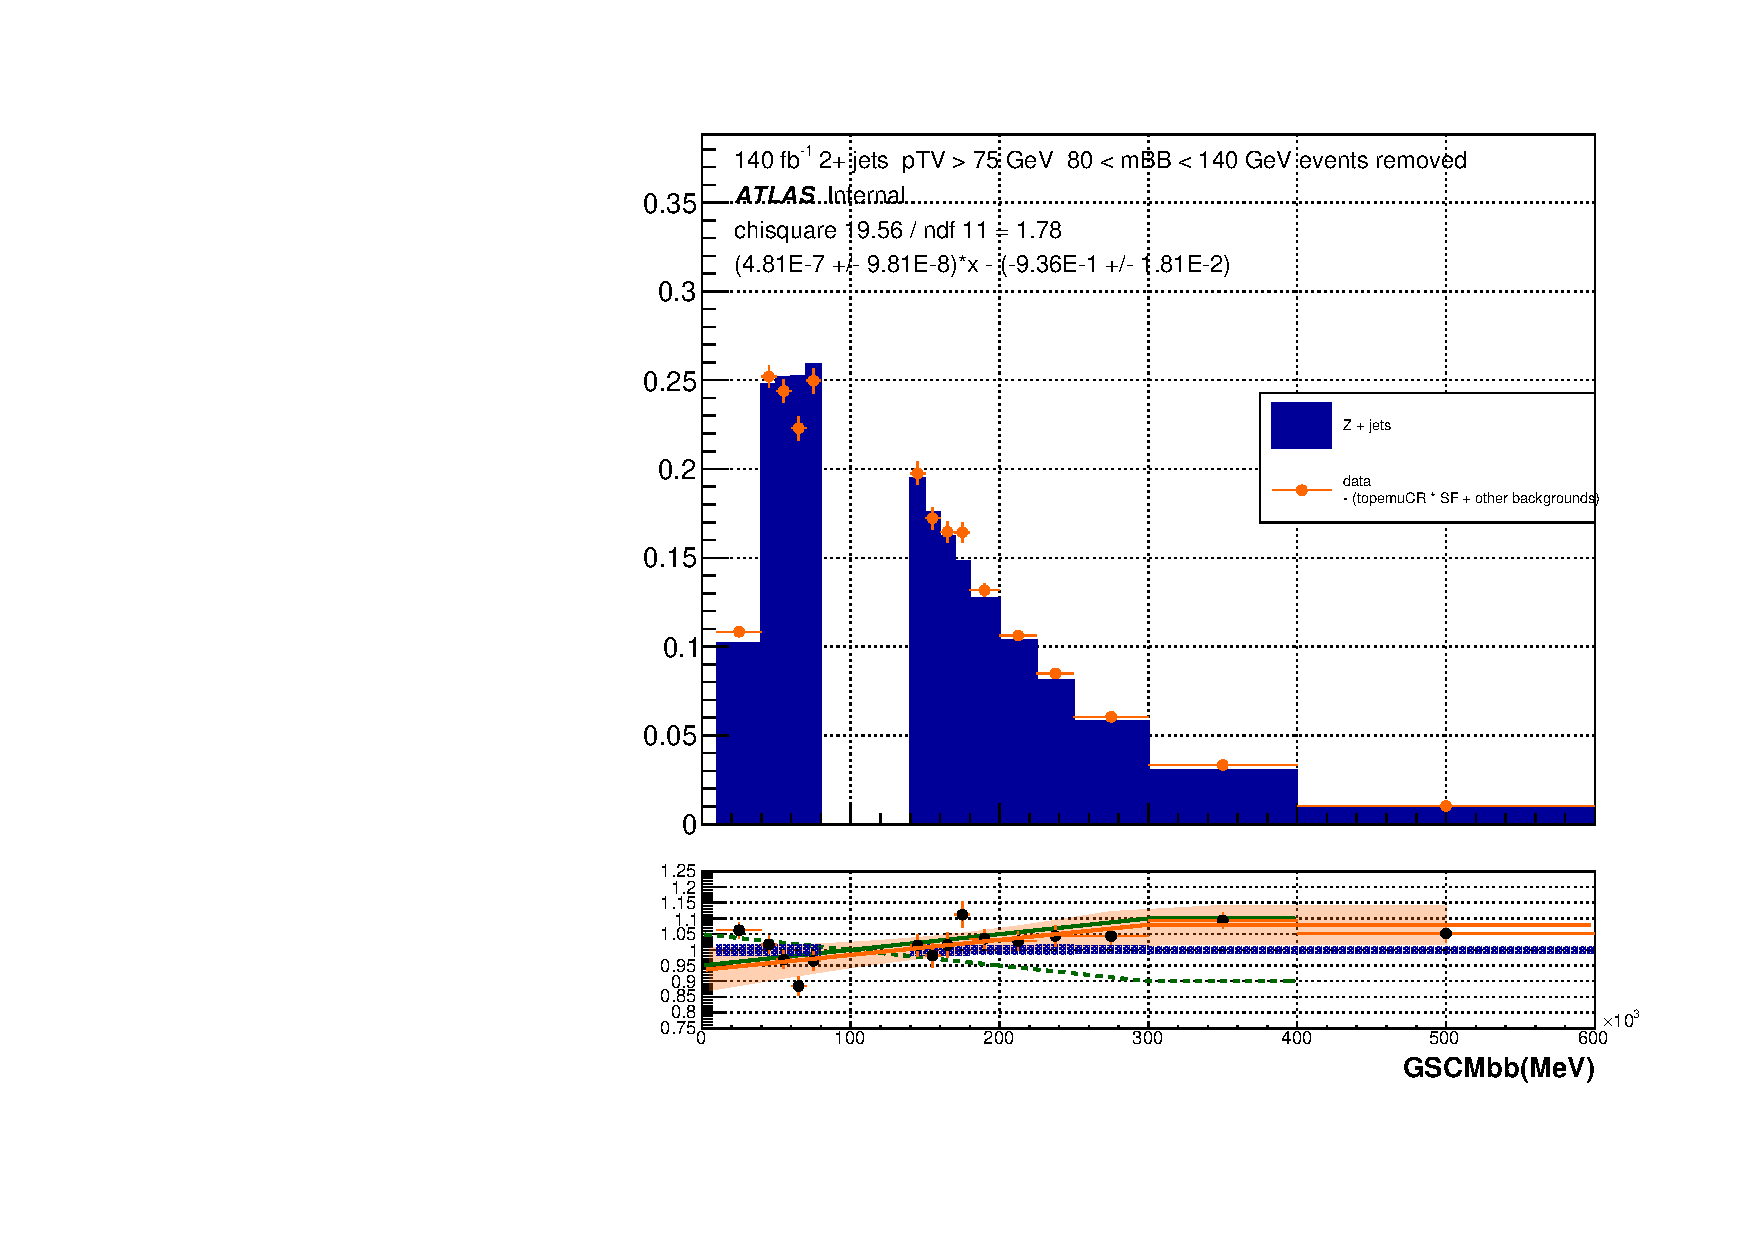
\includegraphics[width=0.59\textwidth]{Zjets-shapes/two_plus_jet_inclusive_blind_ttbardd/two_plus_jet_inclusive_blind_ttbardd_GSCMbb.pdf} \\
  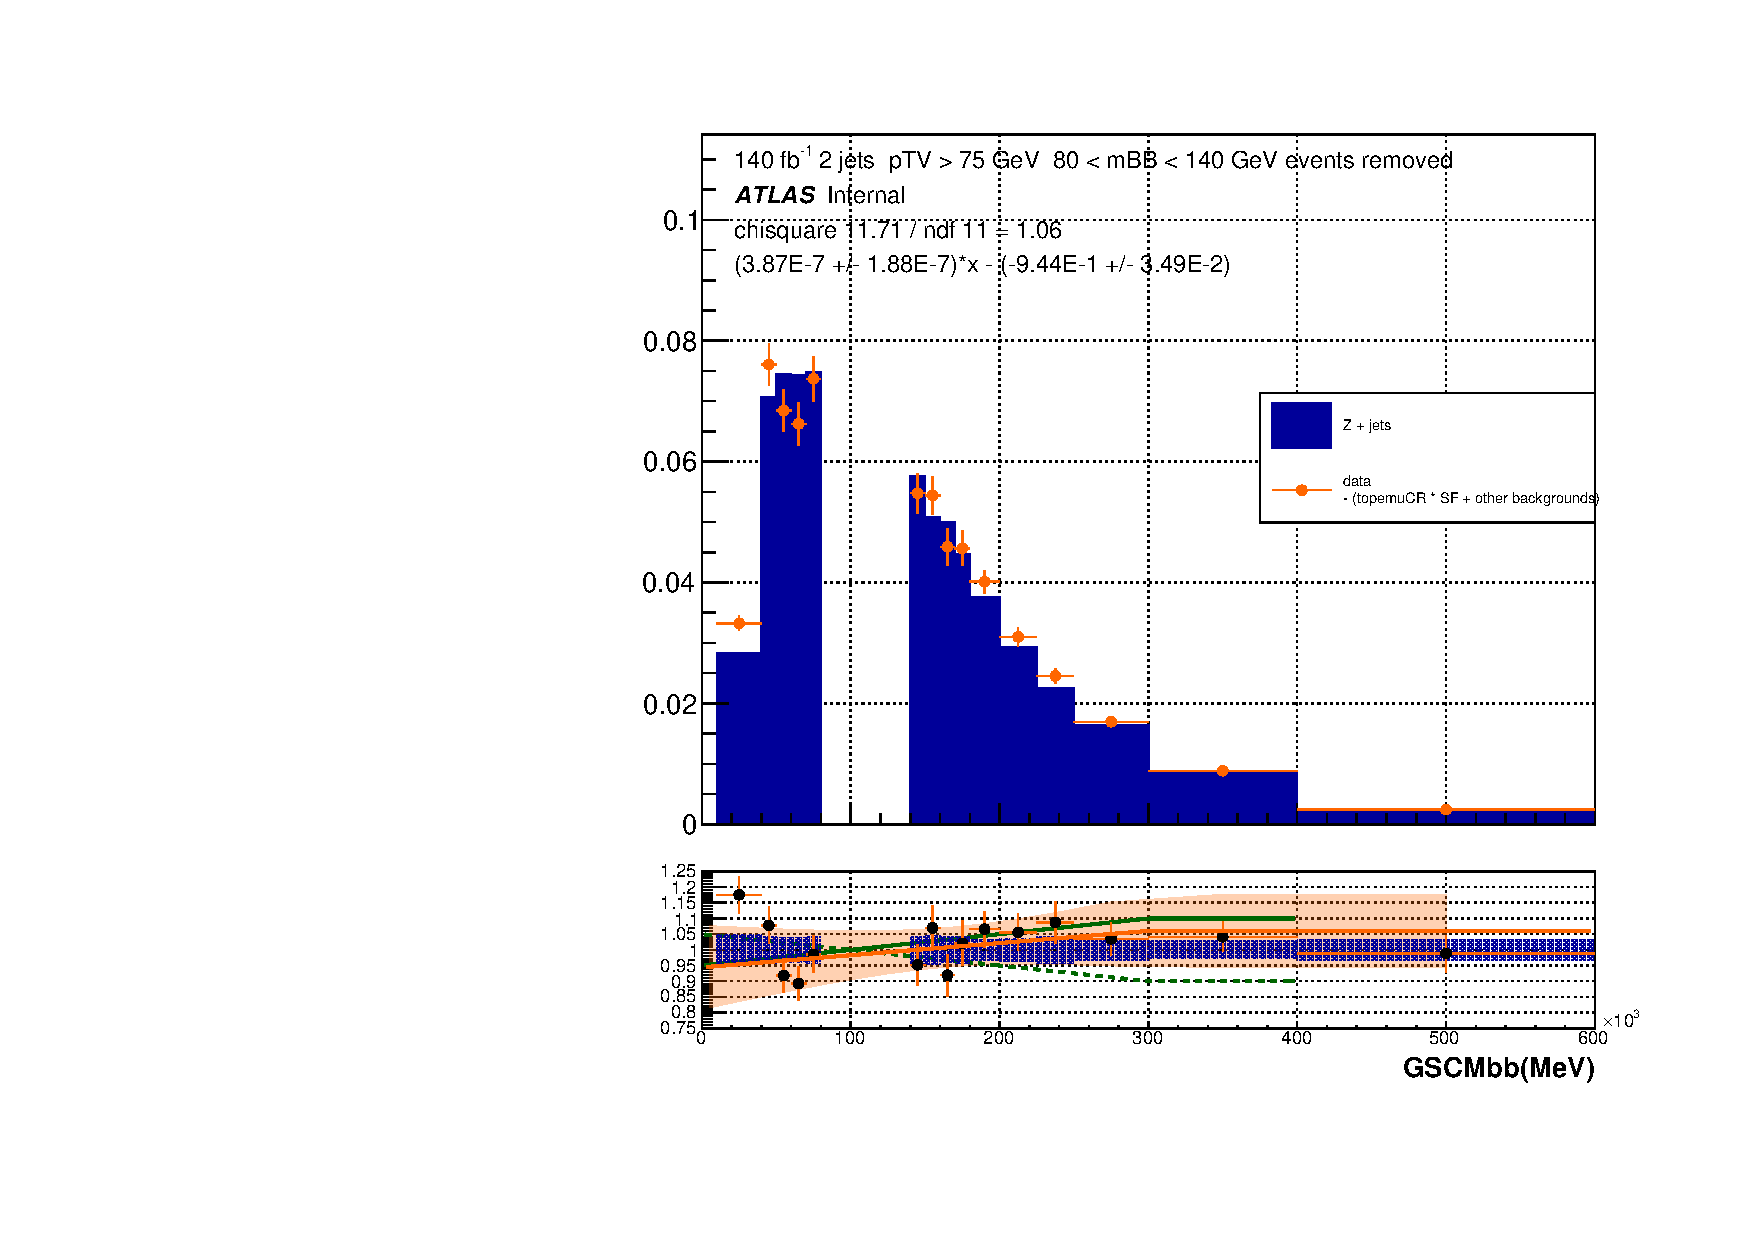
\includegraphics[width=0.59\textwidth]{Zjets-shapes/two_jet_inclusive_blind_ttbardd/two_jet_inclusive_blind_ttbardd_GSCMbb.pdf} \\
  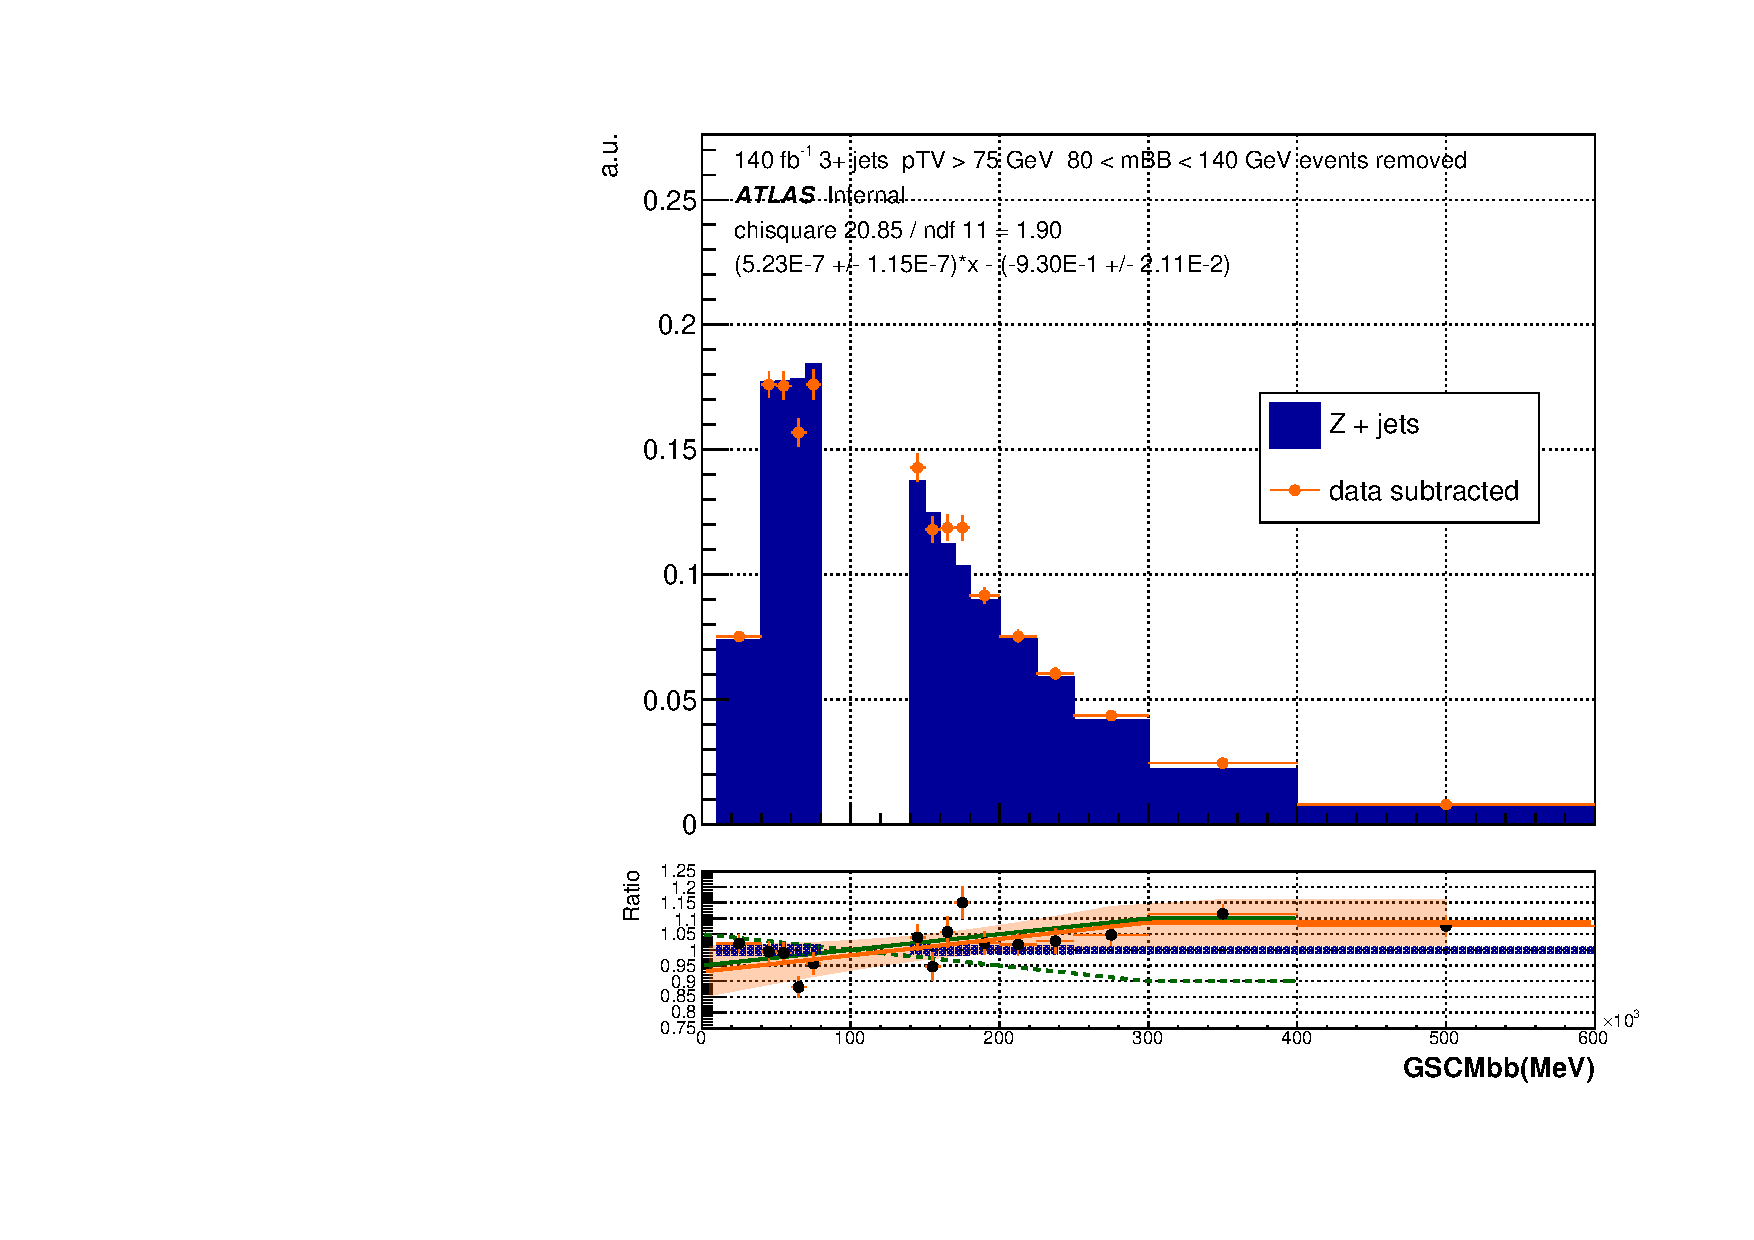
\includegraphics[width=0.59\textwidth]{Zjets-shapes/three_plus_jet_inclusive_blind_ttbardd/three_plus_jet_inclusive_blind_ttbardd_GSCMbb.pdf}
  \caption[Subtracted data versus the nominal $Z+$jets prediction, GSC
  $m_{bb}$.]{Subtracted data versus the nominal $Z+$jets prediction in the GSC
    $m_{bb}$ distribution. The solid and dashed green lines in the ratio panel
    show functional form of the fit used in the previous analysis and it's
    symmetrised version respectively. The solid orange line the ratio is the fit
    to the ratio of the subtracted data and the prediction, the shaded region
    represents the 95~\% confidence interval.}
  \label{fig:zjets-mbb-shapes}
\end{figure}
\begin{figure}[!htb]
  \centering
  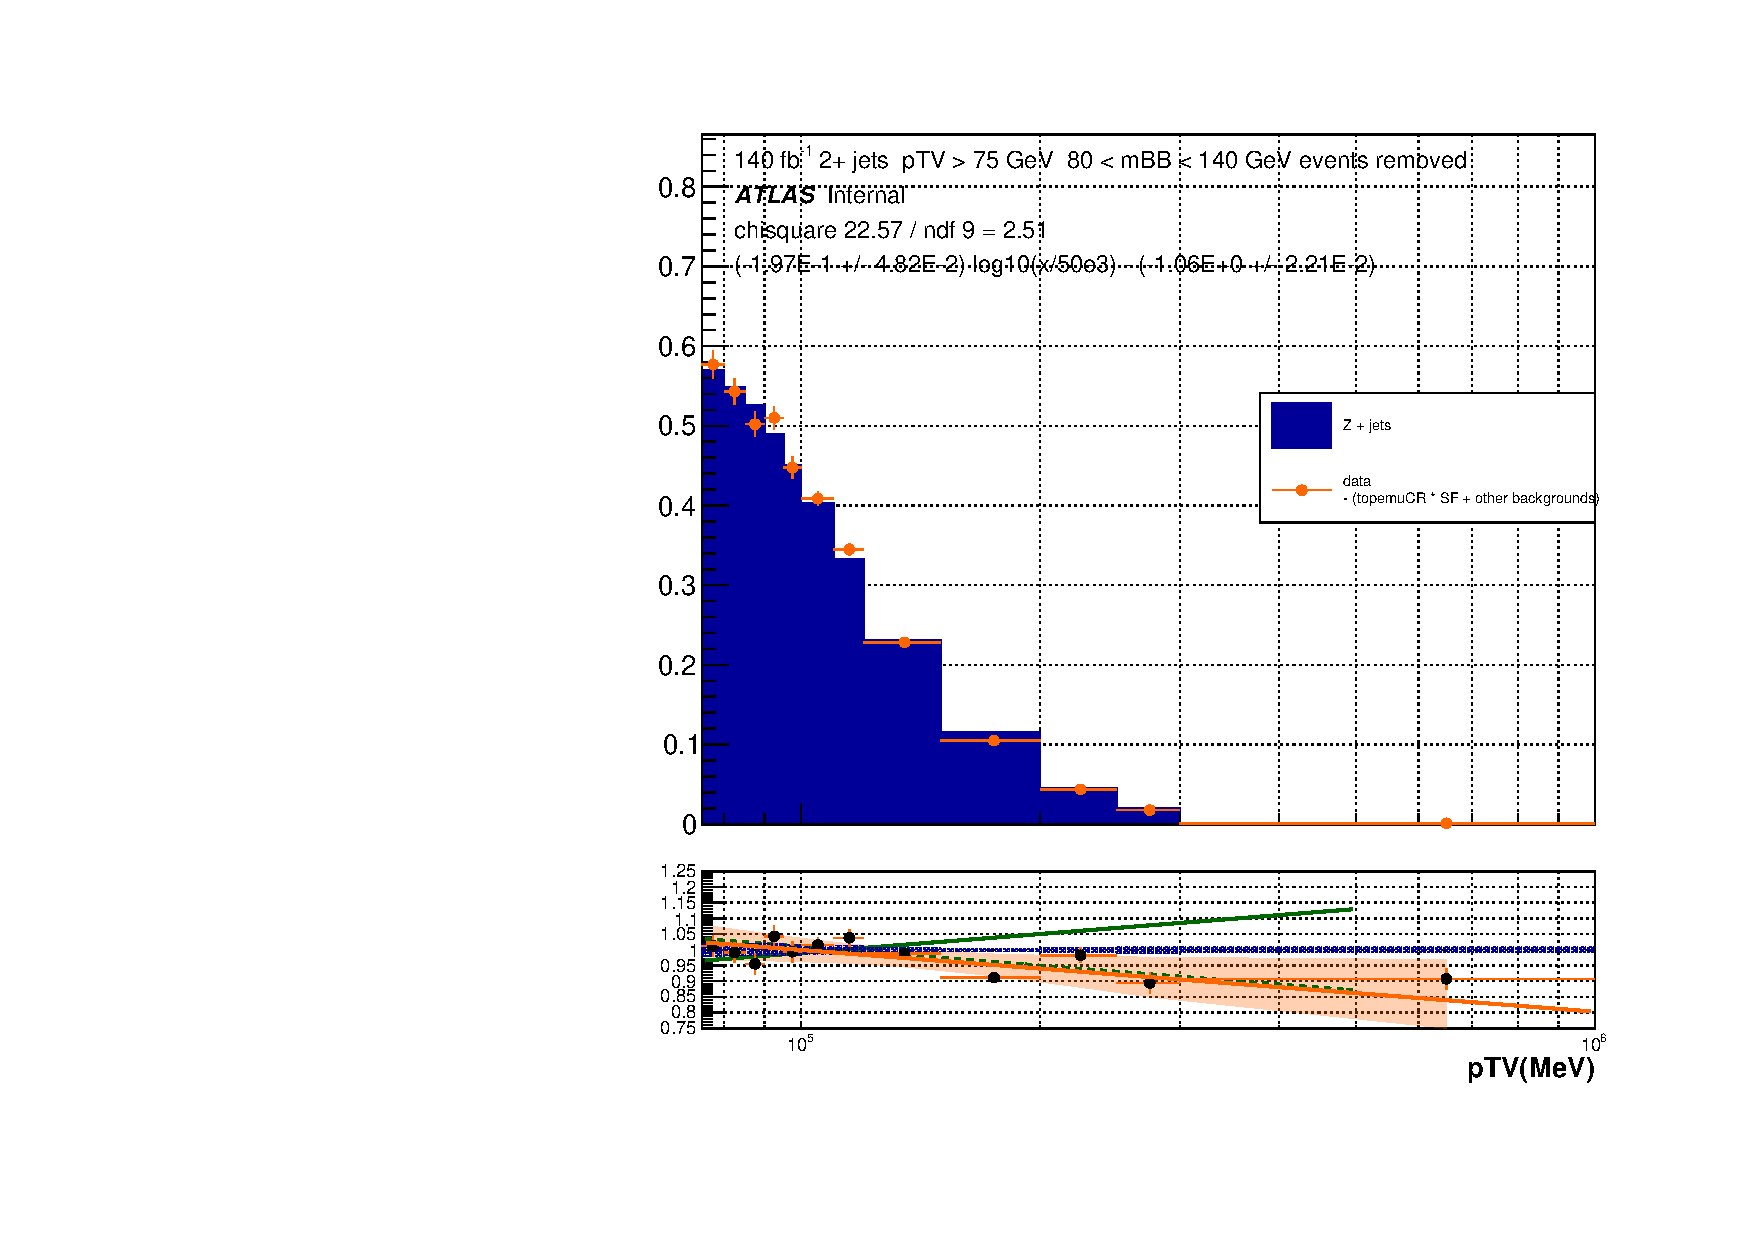
\includegraphics[width=0.49\textwidth]{Zjets-shapes/two_plus_jet_inclusive_blind_ttbardd/two_plus_jet_inclusive_blind_ttbardd_pTV_logx.pdf}
  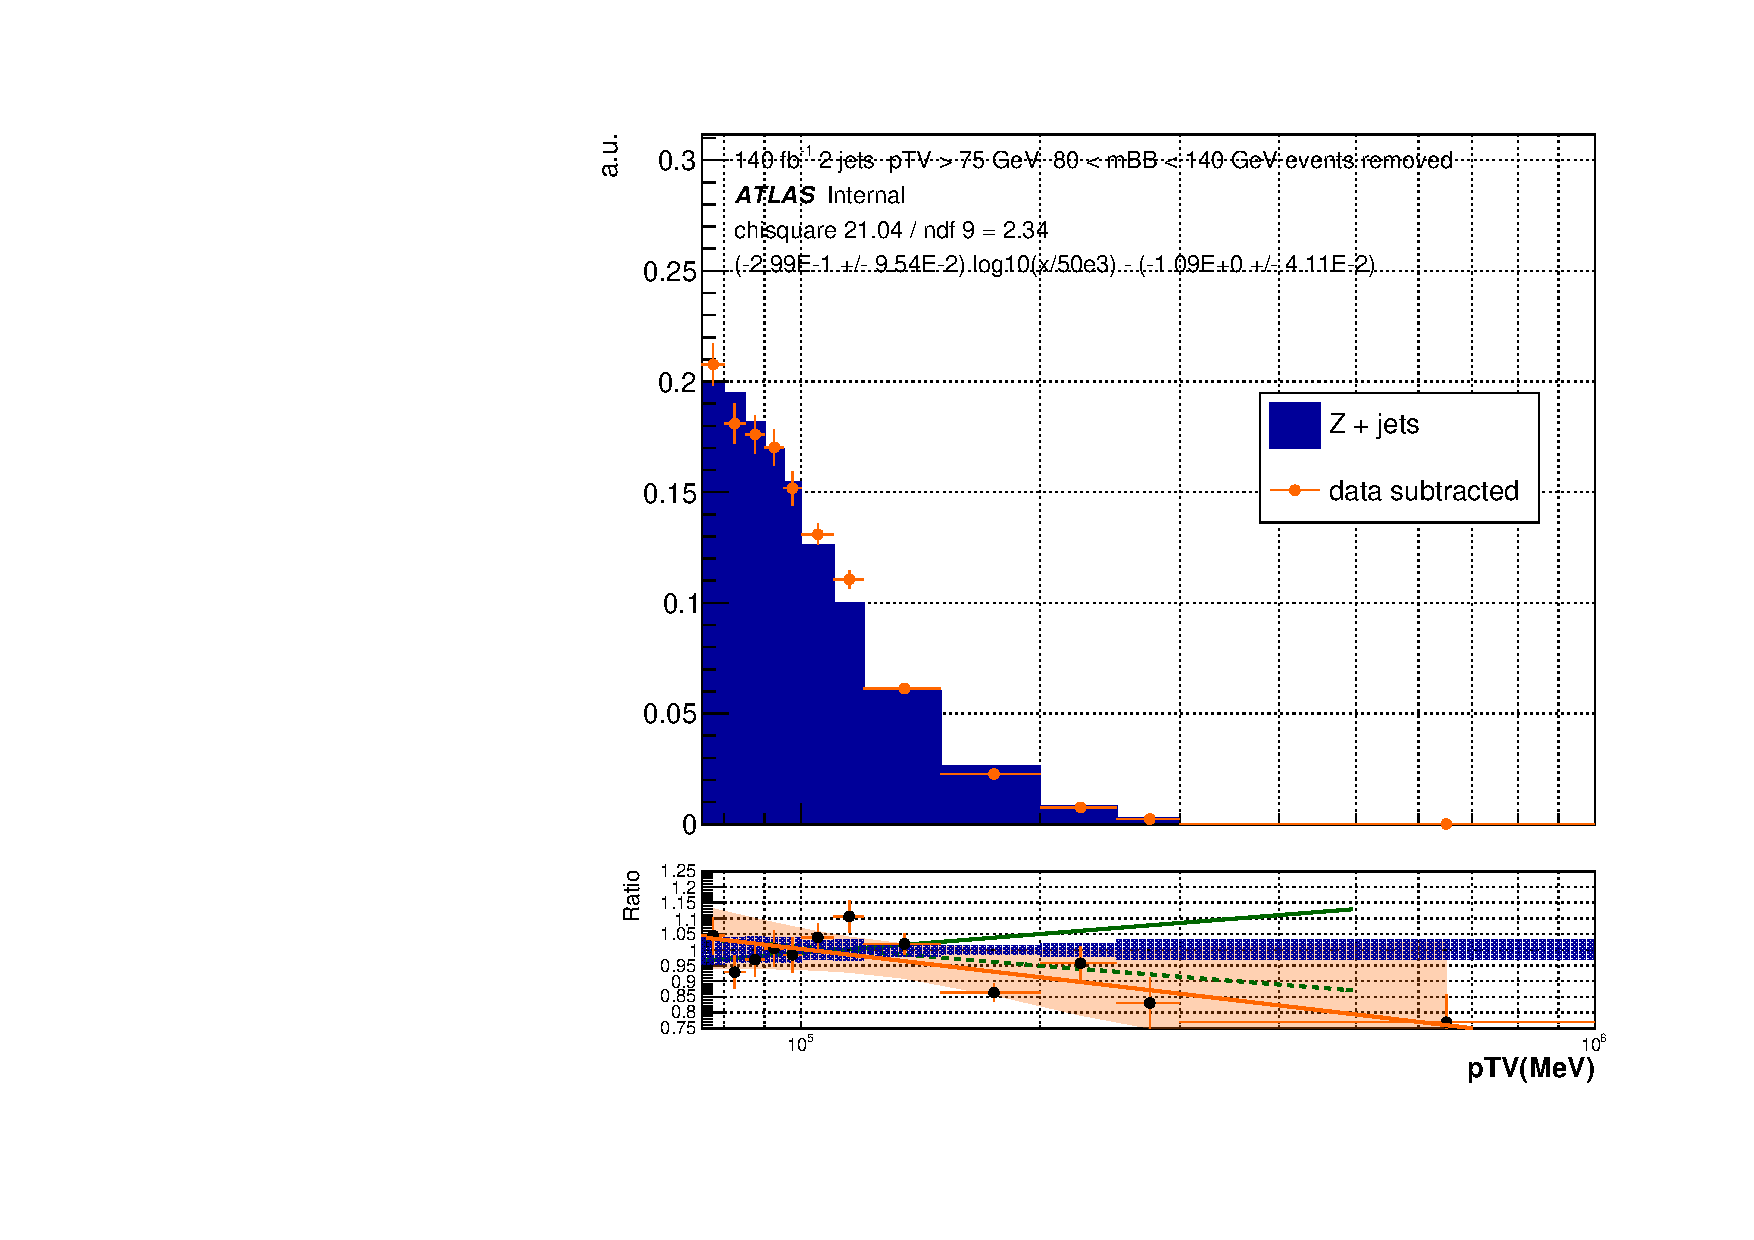
\includegraphics[width=0.49\textwidth]{Zjets-shapes/two_jet_inclusive_blind_ttbardd/two_jet_inclusive_blind_ttbardd_pTV_logx.pdf} \\
  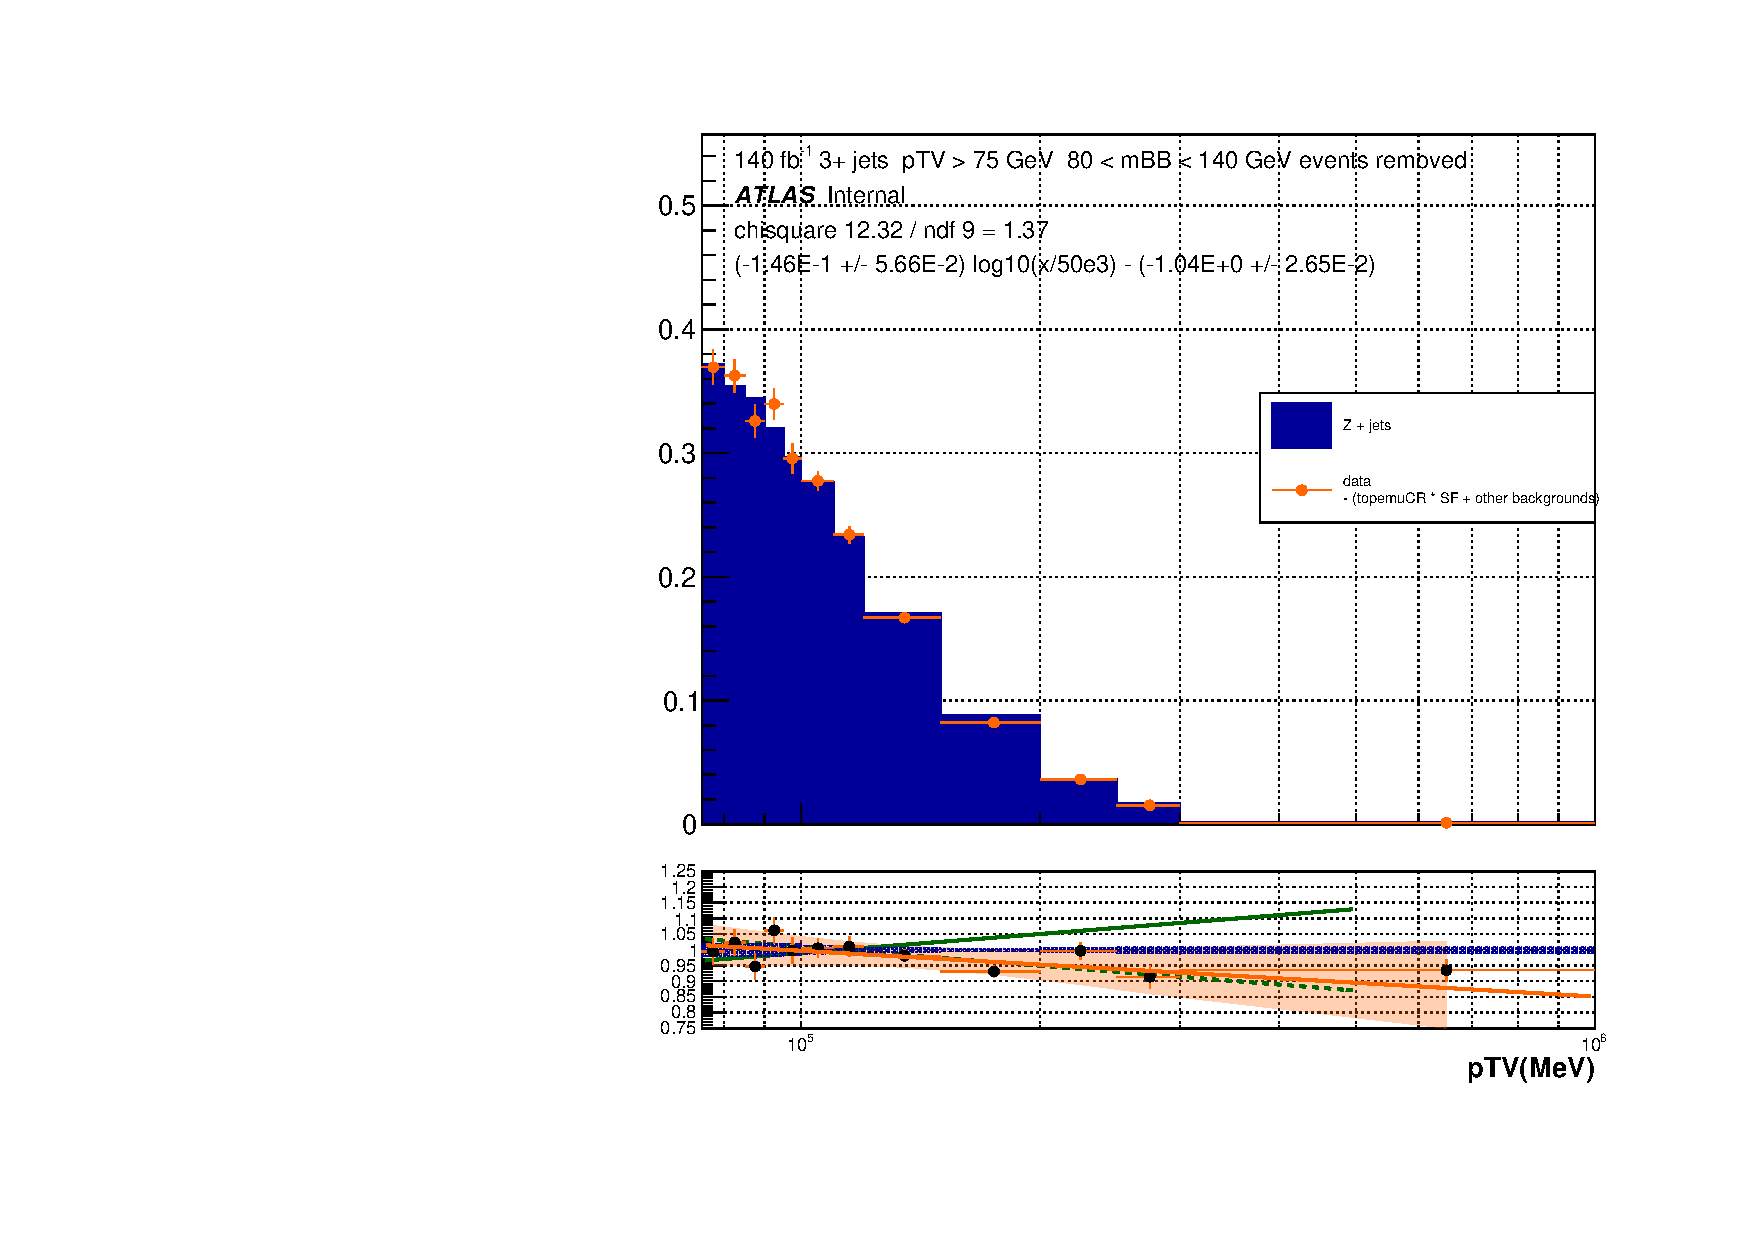
\includegraphics[width=0.49\textwidth]{Zjets-shapes/three_plus_jet_inclusive_blind_ttbardd/three_plus_jet_inclusive_blind_ttbardd_pTV_logx.pdf}
  \caption{The $m_{jj}$ distribution for the 2 lepton $\geq 2$ jets (a), 2-jet
    (b) and $\ge 3$ jets (c) categories.}
  \label{fig:zjets-ptv-shapes}
\end{figure}
The subtracted data is the data with a template comprised of the data from the
top $e\mu$ CR and the nominal predictions of all backgrounds other than Z + jets
subtracted from it. Plots are shown in the 2--jet, $\geq$3--jet and $\geq$2--jet
categories (the sum of the two jet multiplicity based categories in the
analysis) and are plotted across all $p_T^V$ bins of the analysis. The shape
uncertainty is derived by taking a fit to the ratio in the bottom pane of each
plot, the fit defines the 1-$\sigma$ up variation of the Gaussian constrained
nuisance parameter, the symmetrised version of the fit (not displayed) defines
the 1-$\sigma$ down variation. The $\geq$2--jet region is used to calculate the
prior for the systematic uncertainties \texttt{SysZPtV} and \texttt{SysZMbb}
that are applied to all Z + jets events in the 0-- and 2--lepton channels.

The nuisance parameters are correlated across leptonic channels, however as can
be seen by inspection of figure~\ref{fig:zjets-mbb-shapes} the fitted shape does
not cover the discrepancy between the subtracted data and the prediction at low
values of $m_{bb}$. Investigating the plots in
figure~\ref{fig:zjets-mbb-shape-ptv-range} shows that this discrepancy is coming
from the $75~\GeV < p_T^V < 150~\GeV$ analysis bin, therefore the aforementioned
nuisance parameters are decorrelated in this bin.
\begin{figure}[!htb]
  \centering
  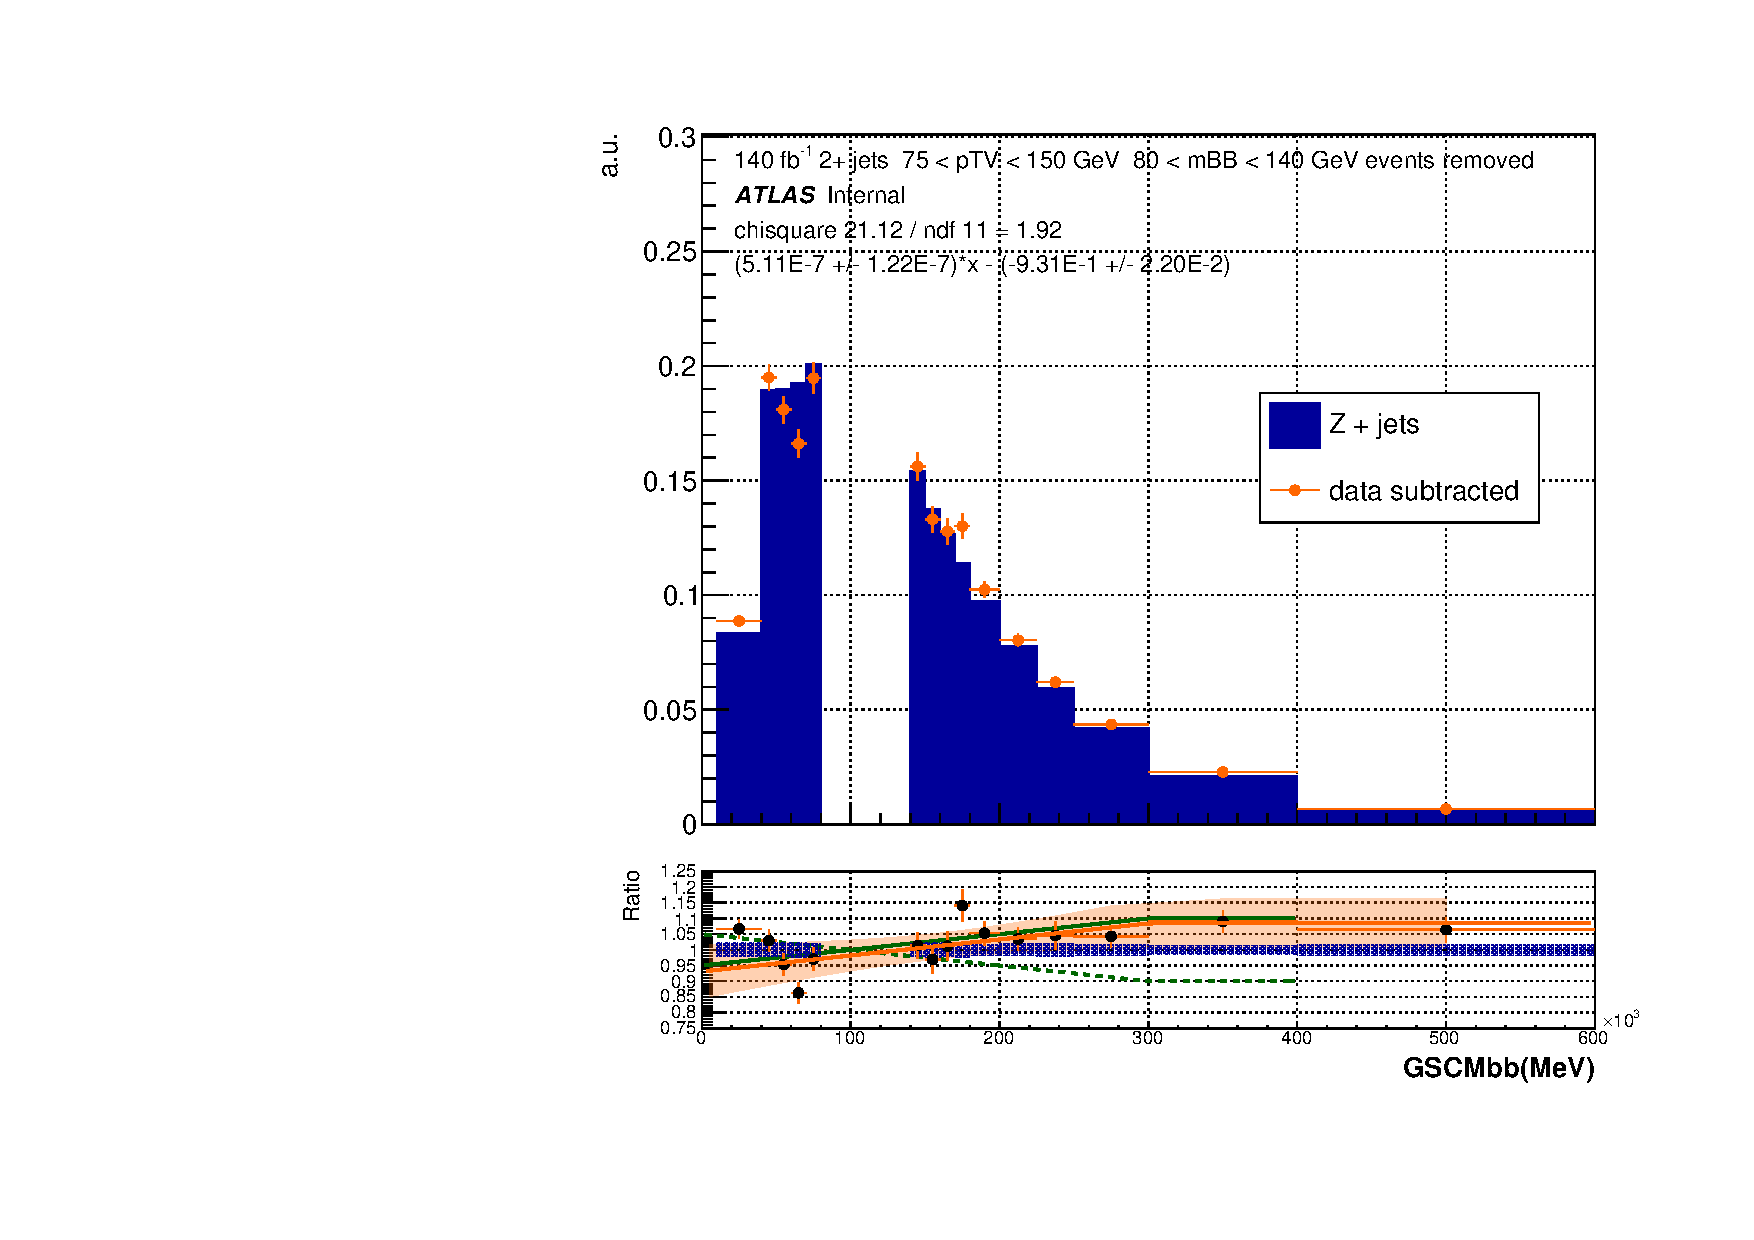
\includegraphics[width=0.59\textwidth]{Zjets-shapes/two_plus_jet_low_blind_ttbardd/two_plus_jet_low_blind_ttbardd_GSCMbb} \\
  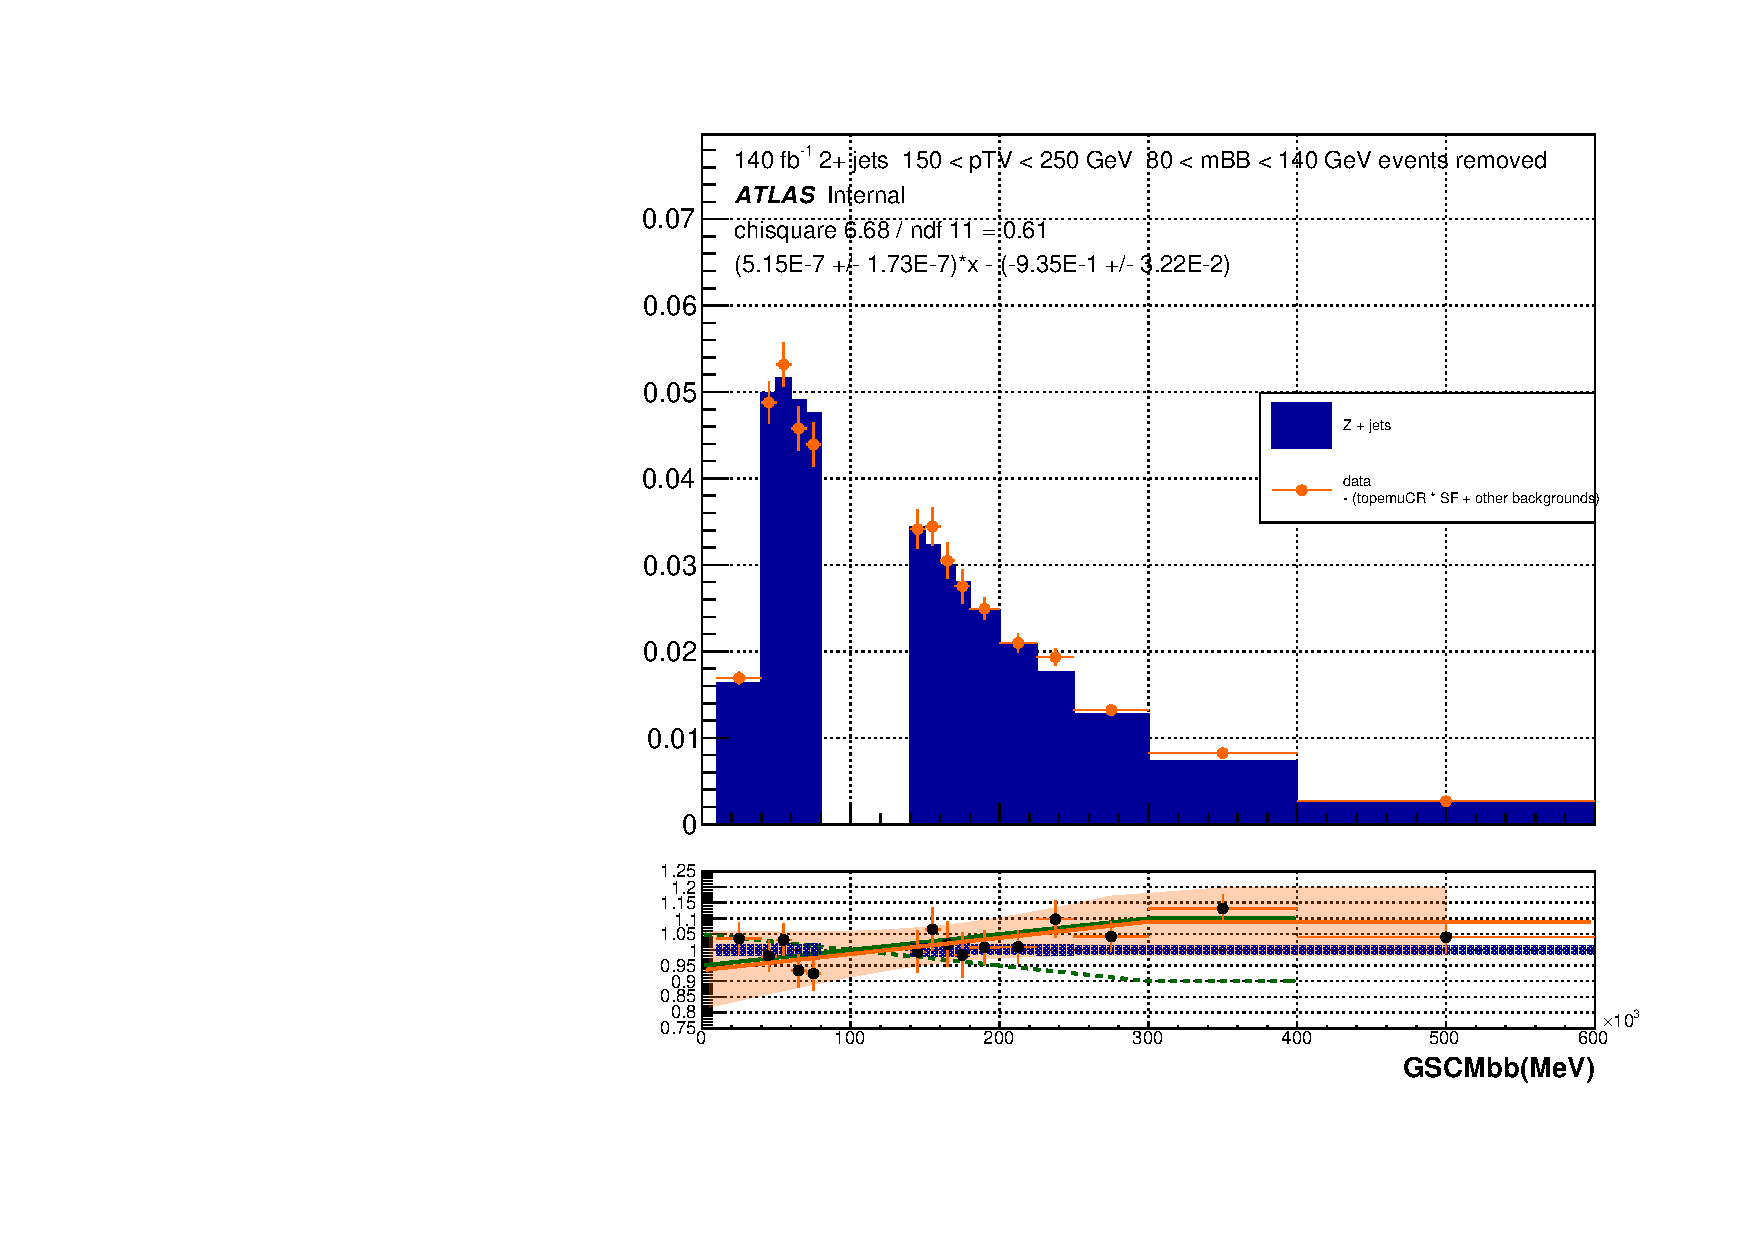
\includegraphics[width=0.59\textwidth]{Zjets-shapes/two_plus_jet_med_blind_ttbardd/two_plus_jet_med_blind_ttbardd_GSCMbb} \\
  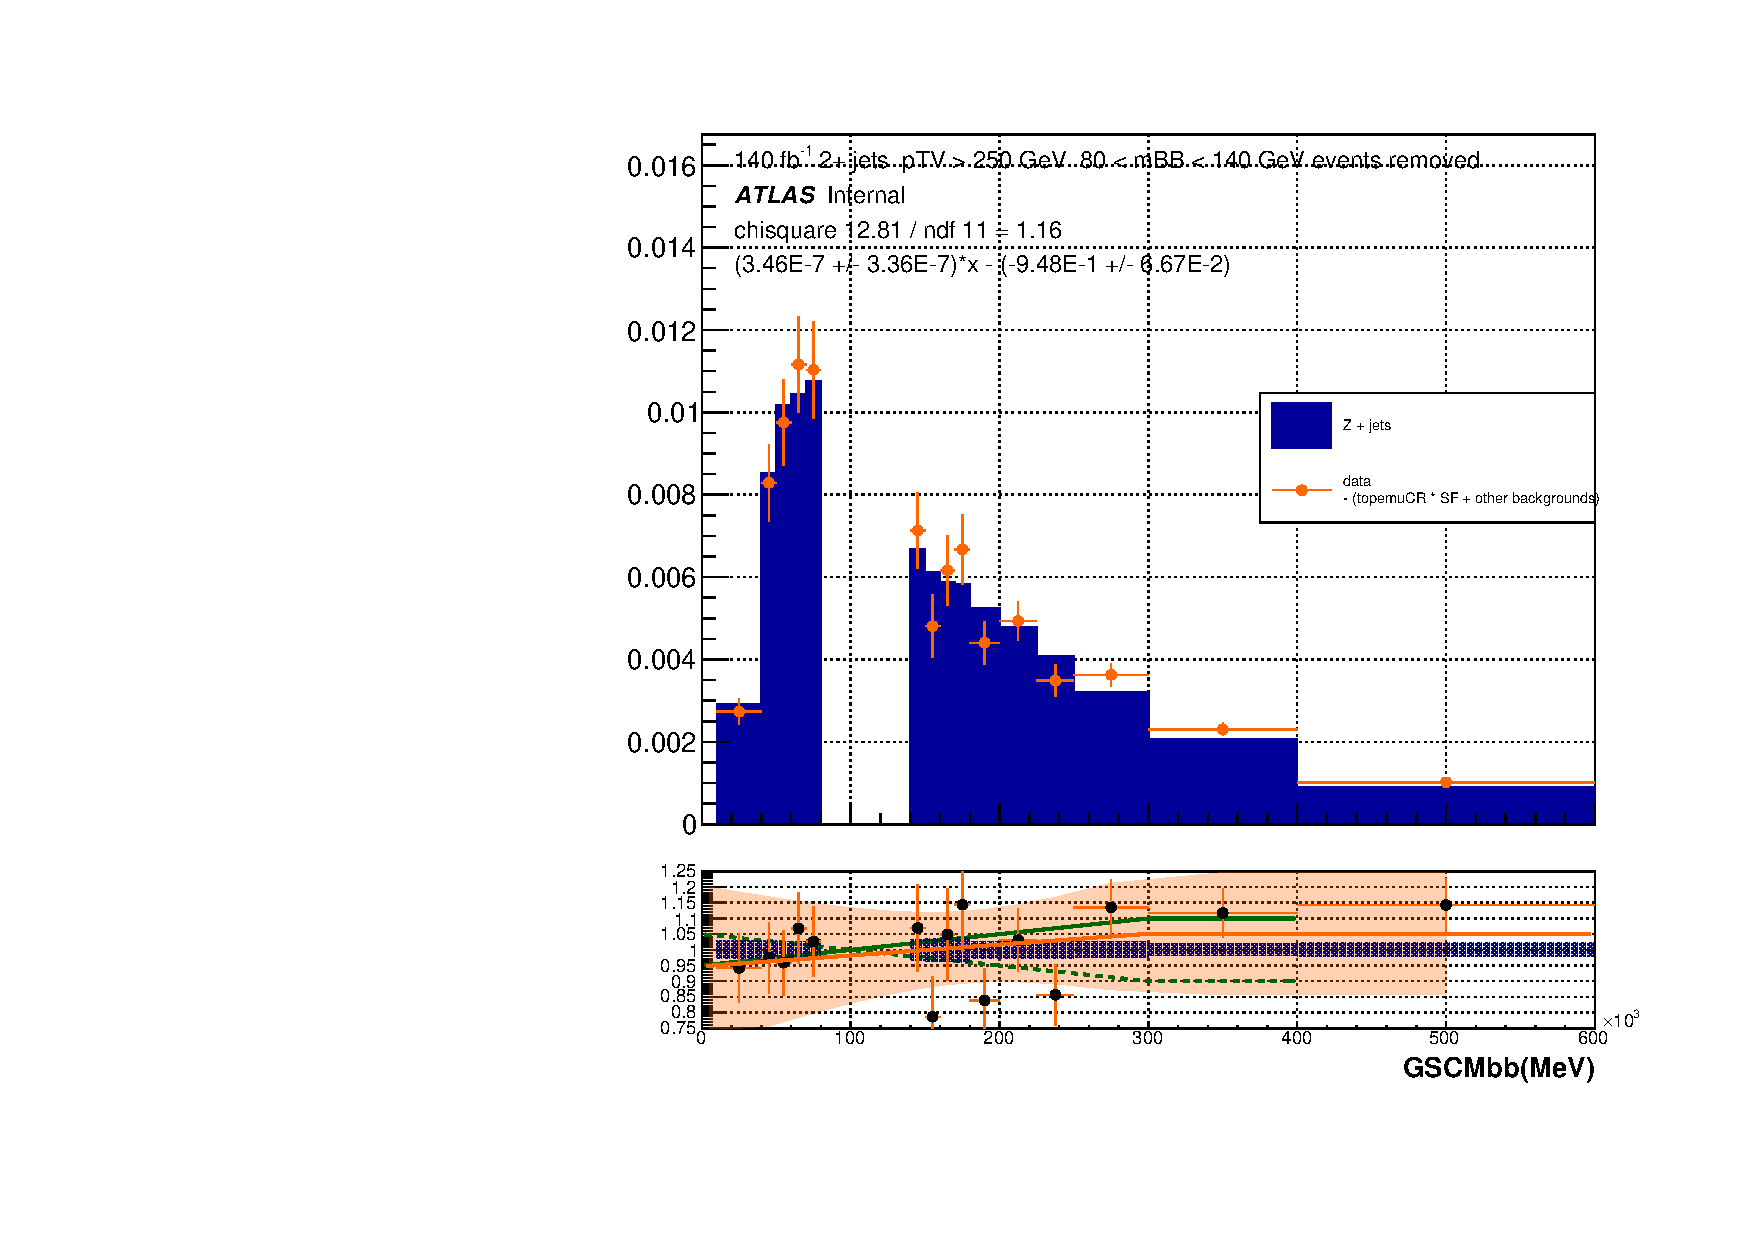
\includegraphics[width=0.59\textwidth]{Zjets-shapes/two_plus_jet_high_blind_ttbardd/two_plus_jet_high_blind_ttbardd_GSCMbb}
  \caption[Subtracted data versus the nominal $Z+$jets prediction, GSC
  $m_{bb}$ across different analysis $p_{\mathrm{T}}^V$ bins.]{Subtracted data
    versus the nominal $Z+$jets prediction in the GSC $m_{bb}$ distribution,
    shown in each of the $p_{\mathrm{T}}^V$ bins of the analysis. The solid and
    dashed green lines in the ratio panel show functional form of the fit used
    in the previous analysis and it's symmetrised version respectively. The
    solid orange line the ratio is the fit to the ratio of the subtracted data
    and the prediction, the shaded region represents the 95~\% confidence
    interval.}
  \label{fig:zjets-mbb-shape-ptv-range}
\end{figure}
The decorrelated parameters are named \texttt{SysZPtV\_BMin75\_L2} and
\texttt{SysMbb\_BMin75\_L2}. A summary of the Z + jets shape uncertainties is
found in table~\ref{tab:zjets-shapes}.
\begin{table}[!htb]
  \resizebox{\textwidth}{!}{%
    \begin{tabular}{lllll}
      \toprule
      {\bfseries Nuisance Parameter} & {\bfseries Uncertainty} & {\bfseries Effect} & {\bfseries Source} & {\bfseries Region} \\
      \midrule
      \texttt{SysZPtV} & $p_T^V$ shape & Shape \& normalisation &  fit to data & All regions with $p_T^V > 150$~\GeV \\
      \texttt{SysZMbb} & $m_{b\bar{b}}$ shape & shape 	& fit to data All regions with $p_T^V > 150$~\GeV \\
      \texttt{SysZPTV\_BMin75\_L2} & $p_T^V$ Shape \& normalisation & fit to data & All regions with $75~\GeV p_T^V < 150$~\GeV \\
      \texttt{SysZMbb\_BMin75\_L2} & $m_{b\bar{b}}$ shape & fit to data & All regions with $75~\GeV p_T^V < 150$~\GeV \\
      \bottomrule
    \end{tabular}
  }
  \caption{A summary of the shape uncertainties for the $Z$+jets background, all
    fits to data take place inclusive of jet multiplicity, $p_T^V$ bin and
    analysis region in the 2--lepton channel.}
  \label{tab:zjets-shapes}
\end{table}

- Shapes derived in CR$_{\text{high}}$ + SR + CR$_{\text{low}}$.
- List of subtracted backgrounds
- What happens to pTV shape when you remove mbb window
- Specifically mention the fit functional form, binning choice, etc. 

\section{Systematic Uncertainties on \texorpdfstring{$t\bar{t}$}{tt} Events}
\label{sec:ttbar-systs}
Modelling of $t\bar{t}$ events differs between the leptonic channels of the
analysis. Like many of the differences between channels that have been discussed
already the reason for this ultimately boils down to there being two visible
charged leptons in the final state of the 2--lepton channel, which come from the
vector boson. Using these charged leptons two regions can be defined in the
2--lepton channel, the same flavour region which breaks down into the usual
CR$_{\text{low}}$, SR and CR$_{\text{high}}$ and the opposite flavour region
known as the top $e\mu$ control region. These regions can be used to get a data
driven estimate of the background from top quark processes in the 2--lepton
channel, described in section~\ref{sec:ttbar_DD} but as they don't exist in the
0-- and 1--lepton channel Monte-Carlo generator predictions and theoretical
uncertainties are used instead. A summary of the nuisance parameters the control
the $t\bar{t}$ systematic uncertainties can be found in
table~\ref{tab:ttbar-systs}.
\begin{table}[hbpt!]
  \resizebox{\textwidth}{!}{
    \begin{tabular}{lllll}
      \toprule
      {\bfseries Nuisance Parameter} & {\bfseries Description} & {\bfseries Categories} & {\bfseries Value}  \\
      \midrule
      {\bfseries Normalisation} & & & & \\
      \texttt{norm\_ttbar\_J2} & Floating $t\bar{t}$ norm     &  $t\bar{t}$, $0/1$--lepton, $2$--jet regions 	& Float	\\
      \texttt{norm\_ttbar\_J3} & Floating $t\bar{t}$ norm     &  $t\bar{t}$, $0/1$--lepton, $3$--jet regions 	& Float	\\
      {\bfseries Acceptance} & & &  \\
      \texttt{SysTTbarNorm\_L0} &  1-- to 0--lep $t\bar{t}$ norm extrapolation     &  0--lepton 	& 8\%	\\
      {\bfseries Flavour Composition}  & & & \\ 
      \texttt{SysTTbarbcMeACC} &  $bc/bb$ acceptance ratio from ME variation & $0/1$--lepton channels & - \\
      \texttt{SysTTbarbcPSACC} &  $bc/bb$ acceptance ratio from PS variation & $0/1$--lepton channels & - \\
      \texttt{SysTTbarOthMeACC} &  $\text{Oth}/bb$ acceptance ratio from ME variation & $0/1$--lepton channels & - \\
      \texttt{SysTTbarOthPSACC} &  $\text{Oth}/bb$ acceptance ratio from PS variation & $0/1$--lepton channels & - \\
      {\bfseries Shape} & & &  \\ 
      \texttt{SysTTbarPtV\_J2} & 0+1--lep $p_{\mathrm{T}}^V$\ shape & $0/1$--lepton channels, 2--jet regions & - \\
      \texttt{SysTTbarPtV\_J3} & 0+1--lep $p_{\mathrm{T}}^V$\ shape & $0/1$--lepton channels, 3--jet regions & - \\
      \texttt{SysBDTr\_ttbar\_ME\_J2} & \textsc{Powheg} to \textsc{MadGraph} multi-variate shape  & $0/1$--lepton channels, 2--jet regions & - \\
      \texttt{SysBDTr\_ttbar\_ME\_J3} & \textsc{Powheg} to \textsc{MadGraph} multi-variate shape & $0/1$--lepton channels, 3--jet regions & - \\
      \texttt{SysBDTr\_ttbar\_PS\_L0} & \textsc{Pythia8} to \textsc{Herwig7} multi-variate shape  & $0$--lepton channel & - \\
      \texttt{SysBDTr\_ttbar\_PS\_Bmin150\_L1} & \textsc{Pythia8} to \textsc{Herwig7} multi-variate shape  & $1$--lepton channel, $150~\GeV< p_{\mathrm{T}}^V <250~\GeV$ & - \\
      \texttt{SysBDTr\_ttbar\_PS} & \textsc{Pythia8} to \textsc{Herwig7} multi-variate shape  & $1$--lepton channel, rest & - \\
      \bottomrule
    \end{tabular}
  }
  \caption[A summary of systematic uncertainties on $t\bar{t}$ events.]{A
    summary of systematic uncertainties of $t\bar{t}$ events. Uncertainties are
    listed by the nuisance parameter that controls them in the profile-likelihood
    fit, a short description is provided for each and the categories in which the
    uncertainty are applied are shown. If a prior is calculated it's value is
    listed. All uncertainties in this table except those under normalisation are
    allowed to affect both the yield and shape of distributions.}
  \label{tab:ttbar-systs}
\end{table}

\paragraph{Nominal and alternative predictions}

The nominal Monte-Carlo prediction for the $t\bar{t}$ process is
\textsc{Powheg}~+~\textsc{Pythia}~8 with the \textsc{Powheg} NLO matrix element
(ME) generator~\cite{JHEP0709.2007.126,JHEP0411.2004.040} interfaced to
\textsc{Pythia}~8~\cite{Comp.Phys.Comm.191.159} using the A14
tune~\cite{ATL-PHYS-PUB-2014-021} to model parton showering, hadronisation,
the underlying event, and multiple parton interactions. The NNPDF3.0 (NLO) and
NNPDF2.3 parton distribution function sets are used in the ME calculation and
parton showering respectively~\cite{ATL-PHYS-PUB-2016-020}.

Details of the samples making up the nominal $t\bar{t}$ prediction can be found
in table~\ref{tab:ttbar-nominal} these include the high and low radiation
variations called  RadHi and RadLo respectively, the samples making up the
alternative prediction can be found in table~\ref{tab:ttbar-alternative}. As
well as accounting for variations in radiation, samples are simulated with
\textsc{Powheg}~+~\textsc{Herwig}~7 to vary the parton shower model and
\textsc{MadGraph}~5\textsc{\_aMC@NLO}+\textsc{Pythia}~8 to vary the matrix
element calculation. 


\paragraph{Cross section}

The $t\bar{t}$ cross section relevant to this analysis is calculated for
proton-proton collisions at a centre of mass energy of $\sqrt{s} = 13$~\TeV and
using a top quark mass of 172.5~\GeV is $831.76^{+40}_{-46}$~pb. The
calculation is  at next-to-next-to leading order in QCD including re-summation
of next-to-next-to-leading logarithmic (NNLL) soft gluon terms with
\textsc{top++2.0}~\cite{Beneke2012695,Cacciari2012612,PhysRevLett.109.132001,NNLOcorr,NNLOcorrNLO,PhysRevLett.110.252004,Czakon:2011xx}.
The PDF and $\alpha_S$ uncertainties are calculated using the PDF4LHC
prescription ~\cite{Botje:2011sn} with the MSTW2008~68\% CL
NNLO~\cite{PDFLHC,alphasunc}, CT10
NNLO~\cite{PhysRevD.82.074024,PhysRevD.89.033009} and NNPDF2.3 5f
FFN~\cite{Ball:2012cx} PDF sets, added in quadrature to the scale uncertainty.
PDFs uncertainties alone correspond to an error of $\pm 35.06$~pb, while
the $\alpha_s$ variations correspond to an error of
$^{+19.77}_{-29.20}$~pb.

\paragraph{Normalisation and Acceptance}

In all fit regions the normalisation of the $t\bar{t}$ background is kept as a
floating normalisation in 2-- and 3--jet categories independently. The nuisance
parameters tracking this normalisation are \texttt{norm\_ttbar\_J2} and
\texttt{norm\_ttbar\_J3} respectively. In terms of acceptance uncertainties,
most of the potential migrations such as migration between analysis regions and
$p_T^V$ bins are covered by the shape uncertainties. There is one nuisance
parameter, \texttt{SysTTbarNorm\_L0} which is implemented to cover migrations
between the 1-- and 0-- lepton channels, it is implemented in the combination of
the 2-- and 3--jet categories, applied to events in the 0--lepton channel and
has a prior calculated using the usual formula in
equation~\ref{eq:acceptance-dr}.

\paragraph{Flavour Composition}

Flavour composition uncertainties are derived using ratios of flavour
sub-components as for other backgrounds, however given that only the $bb$ and
$bc$ sub-components are non-negligible so the remainder of sub-components are
combined into $\text{Oth} = [bl, cc, cl, ll]$. Nuisance parameters are therefore
implemented for $bc$ and Oth only with $bb$ on the bottom of the ratio as
before. Given that neither the matrix element nor parton shower variation
dominates the uncertainty heavily, nuisance parameters are implemented for each
in turn, in total the nuisance parameters controlling flavour composition
uncertainty are \texttt{SysTTbarbcMeACC}, \texttt{SysTTbarbcPSACC},
\texttt{SysTTbarOthMeACC}, \texttt{SysTTbarOthPSACC}.

\paragraph{Shape Uncertainties}

The $(N-1)$--dimensional parametrisation is used to estimate the shape
uncertainties on $t\bar{t}$ events. As in the W + jets the variable that is
factorised out of the multi-dimensional parametrisation is $p_T^V$ which is
chosen for the same reasons as mentioned before. The shape systematic is not as
correlated over as many of the analysis bins as in the W + jets case. The
$p_T^V$ shape uncertainty is correlated across 0-- and 1--lepton channels but
decorrelated in jet multiplicity as \texttt{SysTTbarPtV\_J2} and
\texttt{SysTTbarPtV\_J3} for the 2-- and 3--jet categories respectively. The
$p_T^V$ shapes used are coming from the largest variation when considering all
samples which turns out to be the comparison of
\textsc{Powheg}~+~\textsc{Pythia}~8 and
\textsc{MadGraph}~5~\textsc{\_aMC@NLO}~+~\textsc{Pythia}~8. The BDTr shape
uncertainty is not clearly dominated by one comparison of generators and
therefore multiple nuisance parameters enter to encapsulate all the potential
sources of uncertainty. Differences due to the matrix element calculation are
correlated in leptonic channel but decorrelated in 2-- and 3--jet categories as
\texttt{SysBDTr\_ttbar\_ME\_J2} and \texttt{SysBDTr\_ttbar\_ME\_J3}
respectively. For the parton shower variation the uncertainties are correlated
in jet multiplicity but decorrelated in leptonic channel and also in the
1--lepton channel decorrelated in $p_T^V$ bin, the nuisance parameters in
question are \texttt{SysBDTr\_ttbar\_PS\_L0},
\texttt{SysBDTr\_ttbar\_PS\_Bmin150\_L1}, and \texttt{SysBDTr\_ttbar\_PS}.

\subsection{Data Driven Estimation}
\label{sec:ttbar_DD}

As mentioned in section~\ref{sec:topemucr} the top $e\mu$ control region is
constructed and studied in the analysis in order to get a handle on top quark
backgrounds in the 2--lepton channel. Due to the flavour symmetry of the
$t\bar{t}$ and $Wt$ processes the shape of the top quark backgrounds in the top
$e\mu$ control region and the SR ought to be the same. In order to correct for
any differences in normalisation a scale factor $\alpha$ is derived as follows
\begin{align}
  N_{\text{top, data}}^{\text{SR}}
  =
  \frac{N_{\text{top, MC}}^{\text{SR}}}{N_{\text{top, MC}}^{\text{CR}}}
  \times
  N_{\text{top, data}}^{\text{ CR}}
  = \alpha \times N_{\text{top, data}}^{\text{ CR}}.
  \label{eq:TTbar_DD_ExtrapFac}
\end{align}
Once that factor is applied then the data from the top $e\mu$ control region can
be used as a template for top quark backgrounds in the SR.

Using the data driven estimate of the background eliminates the need to apply
the experimental systematics detailed in section~\ref{sec:experimental-systs}
which are related to detector performance, jet reconstruction and flavour
tagging. It also means we don't have to consider theoretical modelling
uncertainties associated with any Monte-Carlo generator. Note that systematic
uncertainties on the Monte-Carlo prediction used to derive the scale factor
$\alpha$ cancel.

In order to check the validity of this approach a data versus prediction check
was carried out as part of series of wider checks~\cite{VHModellingNote2019}.
This check includes the data from the top $e\mu$ control region as the
prediction for both $t\bar{t}$ and single top events. The plots showing the
comparison can be found in figure~\ref{fig:ttbar-mbb}.
% \begin{figure}[hpbt!]
% 	\begin{center}
% 		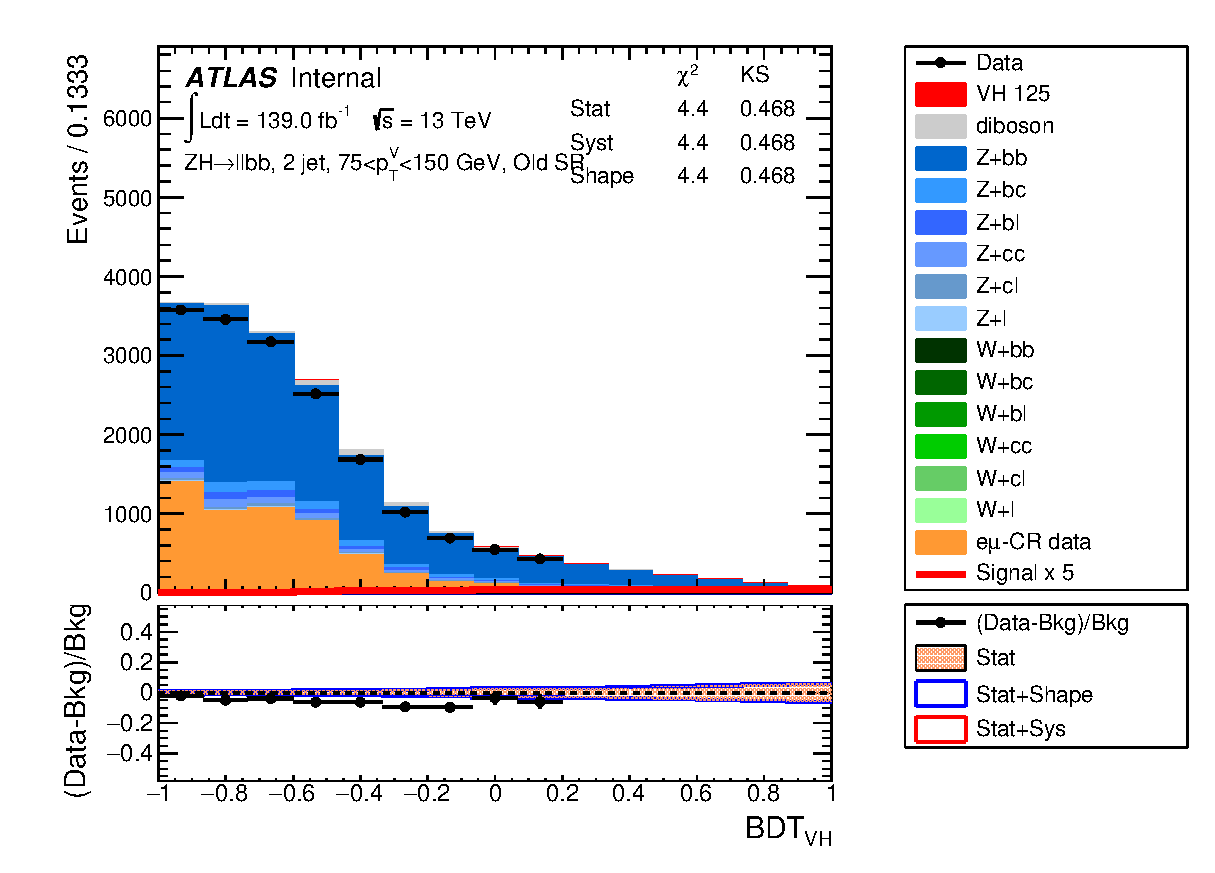
\includegraphics[width=75mm]{\ddtt@figures/dataMC_ade/C_2tag2jet_75_150ptv_SROld_mva_trafo.eps}
% 		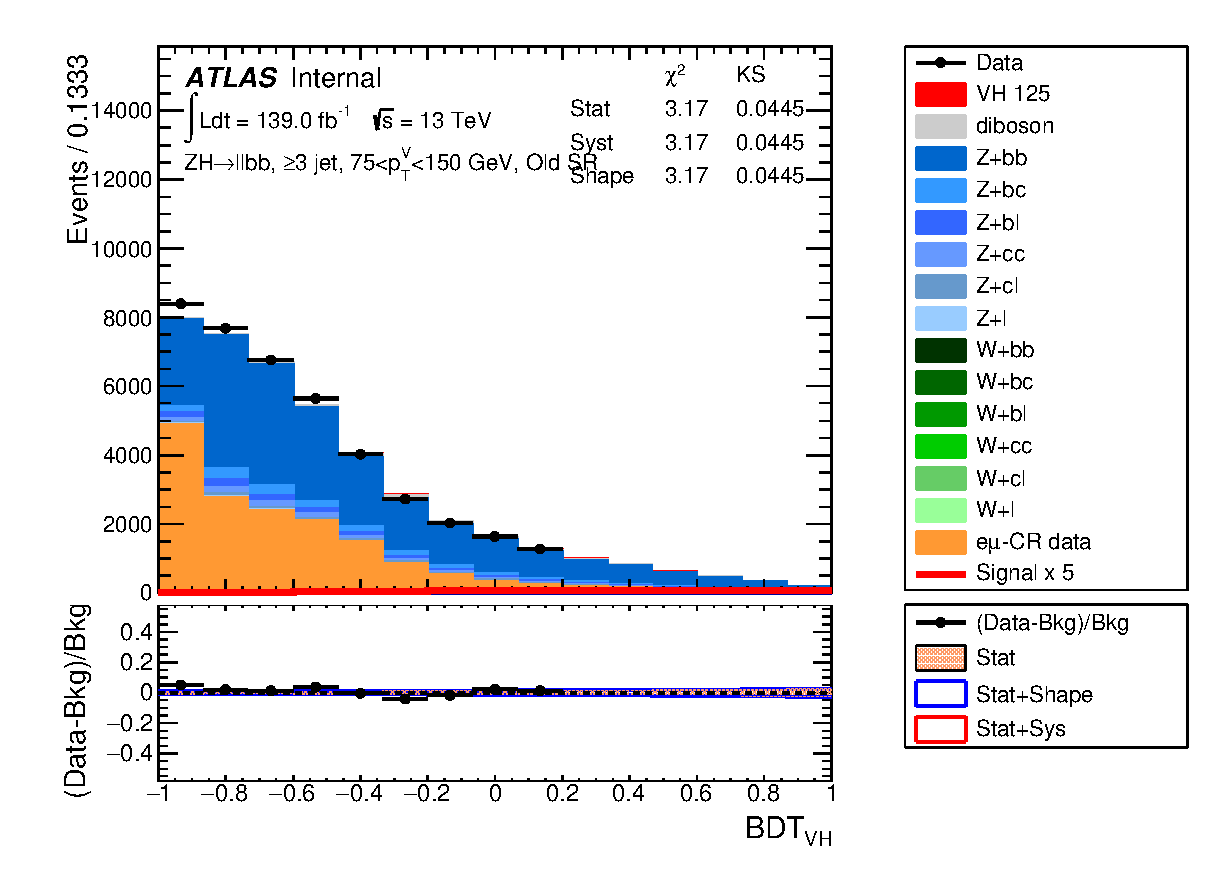
\includegraphics[width=75mm]{\ddtt@figures/dataMC_ade/C_2tag3pjet_75_150ptv_SROld_mva_trafo.eps}
% 		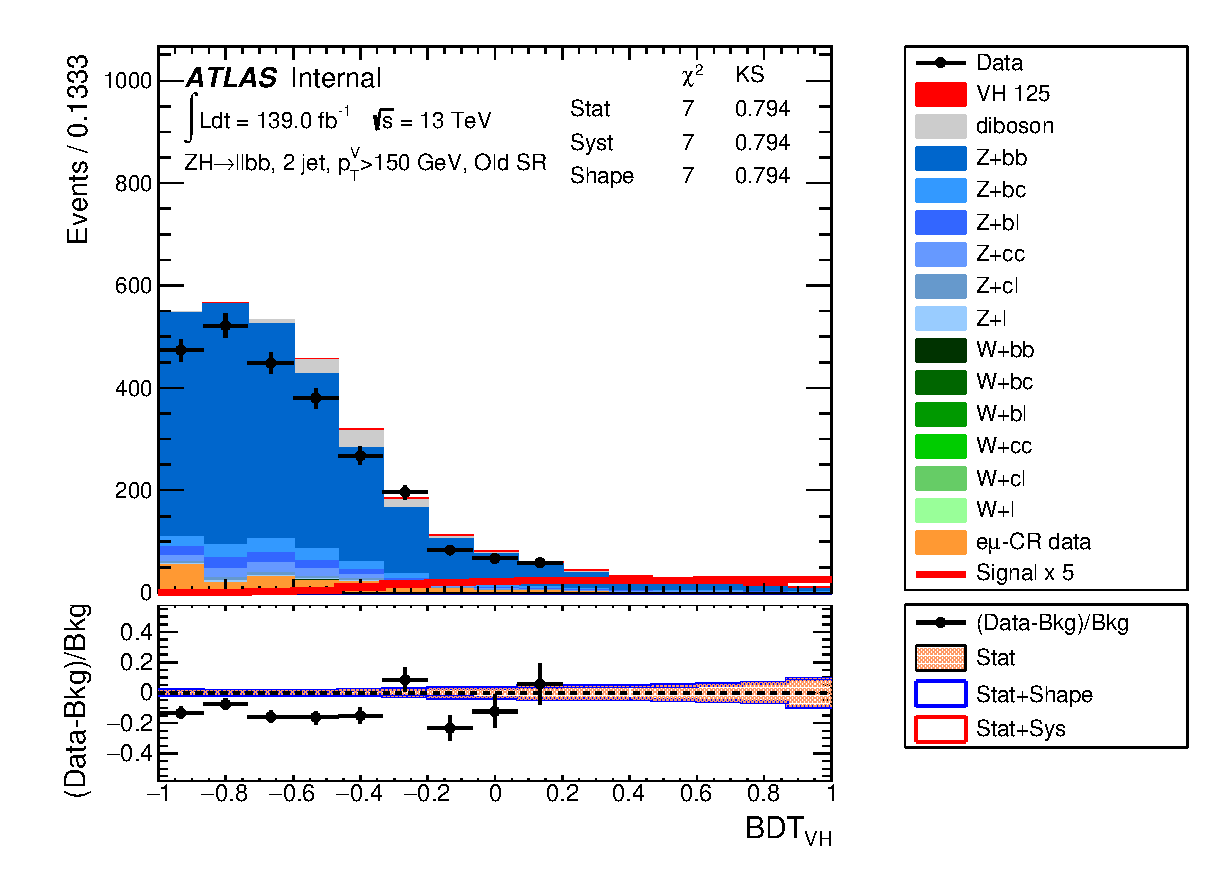
\includegraphics[width=75mm]{\ddtt@figures/dataMC_ade/C_2tag2jet_150ptv_SROld_mva_trafo.eps}
% 		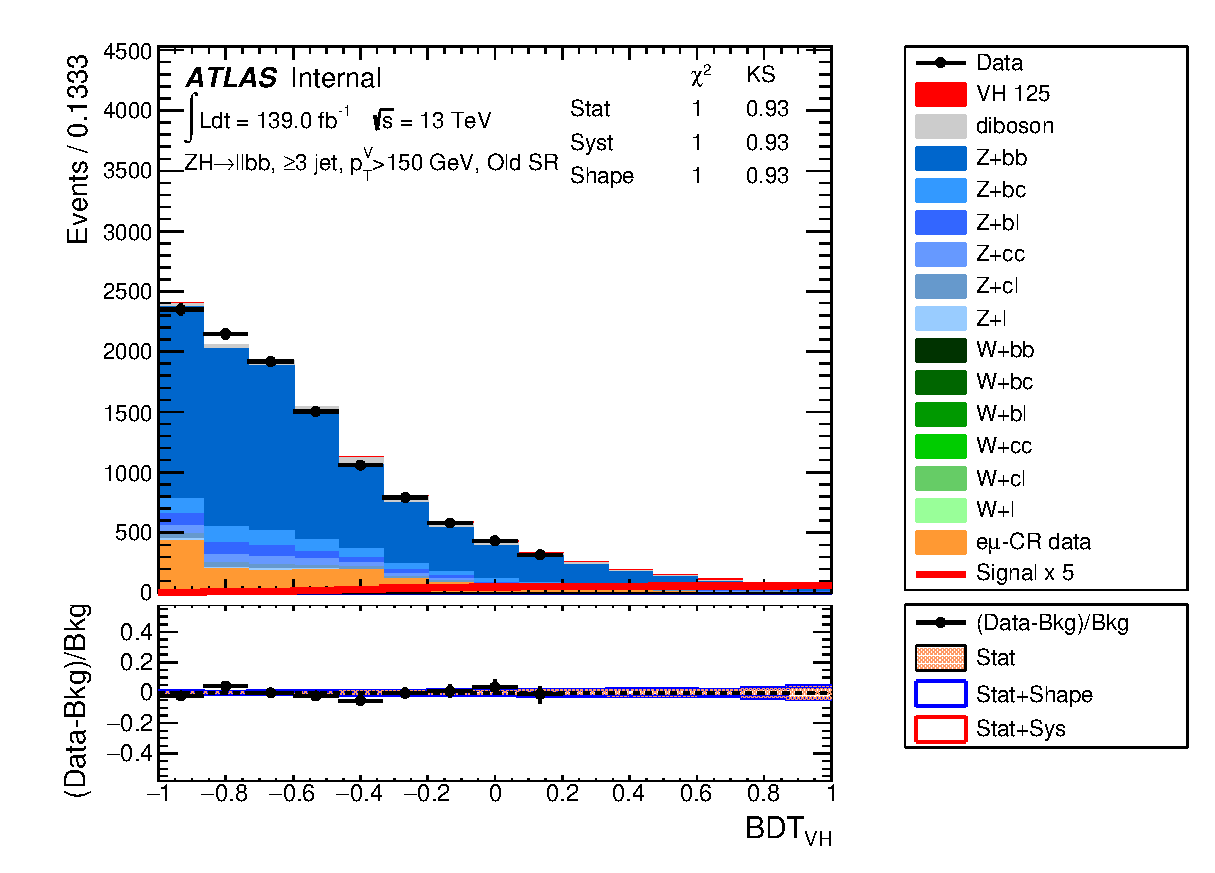
\includegraphics[width=75mm]{\ddtt@figures/dataMC_ade/C_2tag3pjet_150ptv_SROld_mva_trafo.eps}				
% 	\end{center}
% 	\caption{Data-MC comparison of BDT output distributions in SR in each \ptv{} and nJet bin.}
% 	\label{fig:DataMCmva}
% \end{figure}
\begin{figure}[hpbt!]
	\centering
  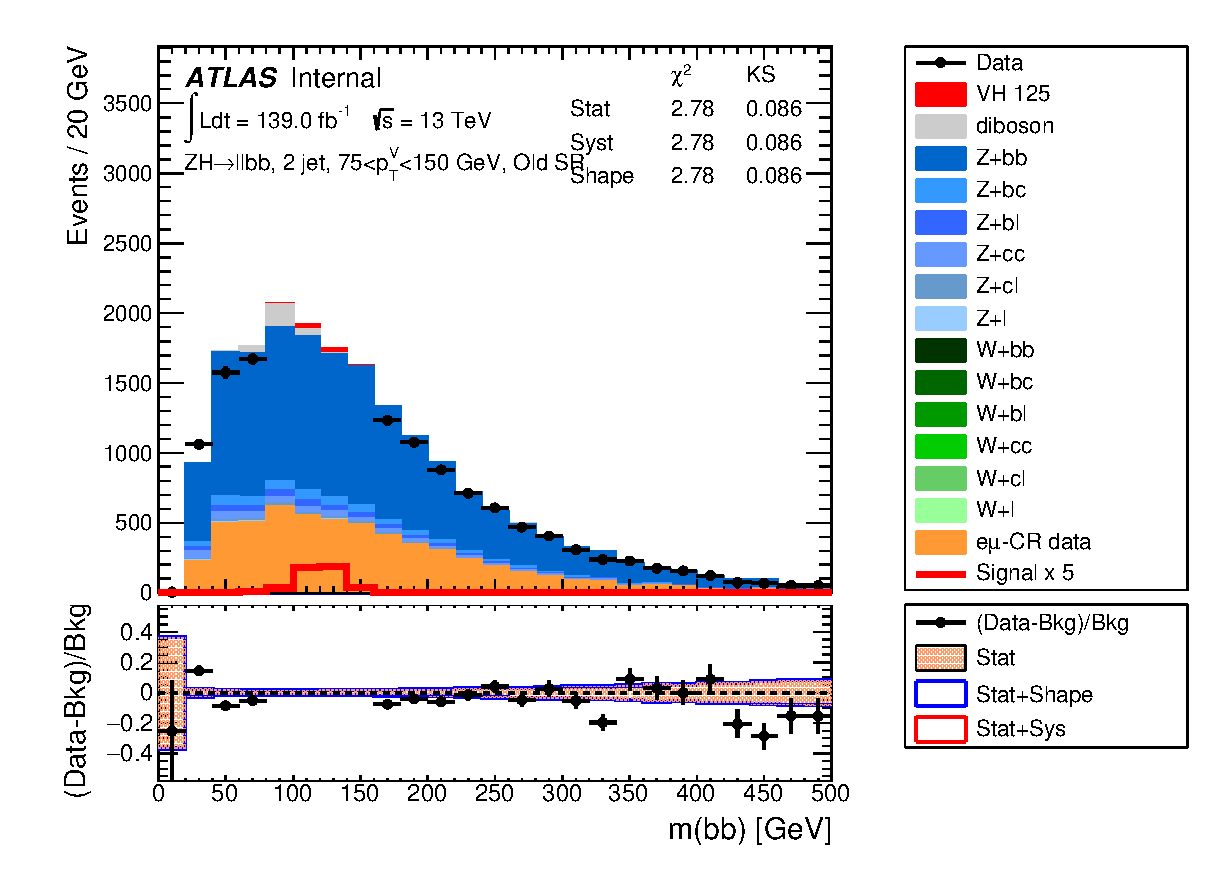
\includegraphics[width=75mm]{dataMC_ade/C_2tag2jet_75_150ptv_SROld_mBB.eps}
  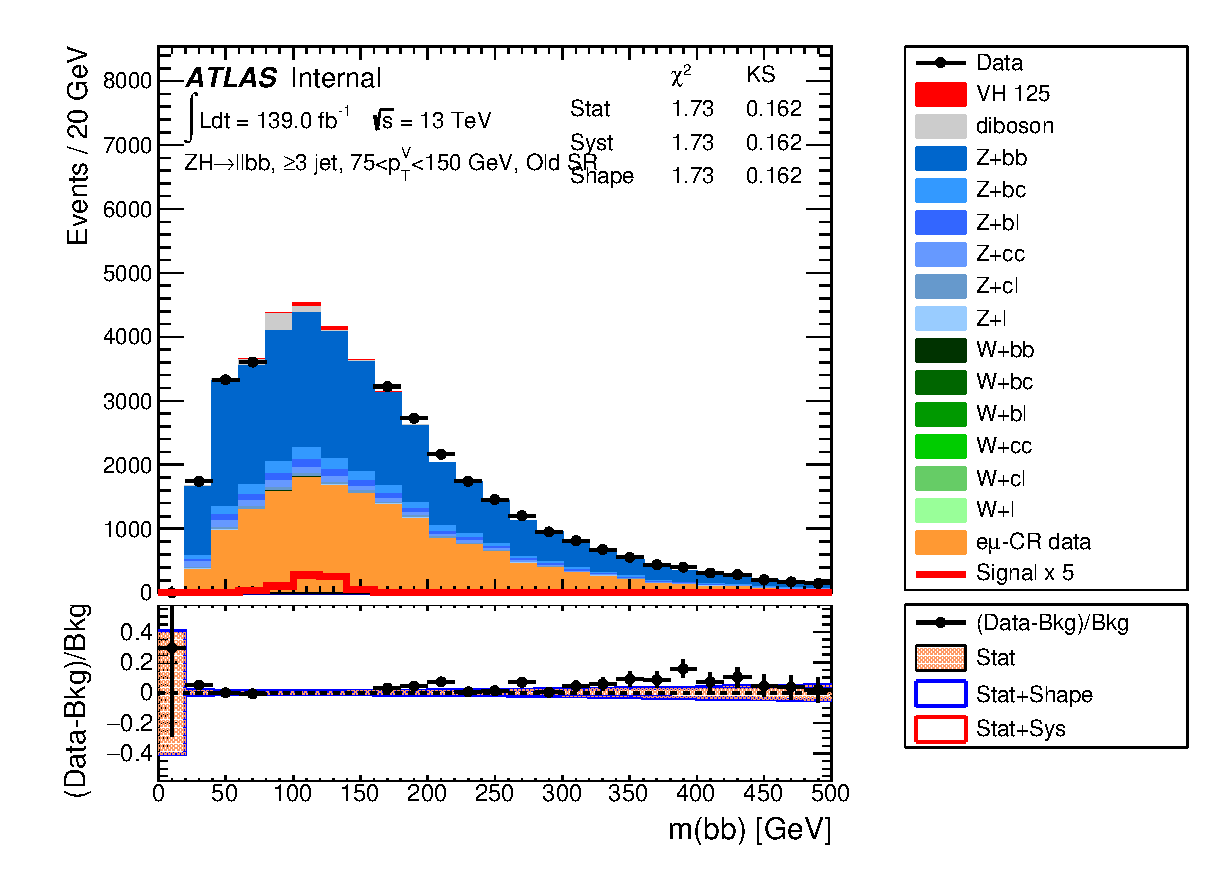
\includegraphics[width=75mm]{C_2tag3pjet_75_150ptv_SROld_mBB.eps}
  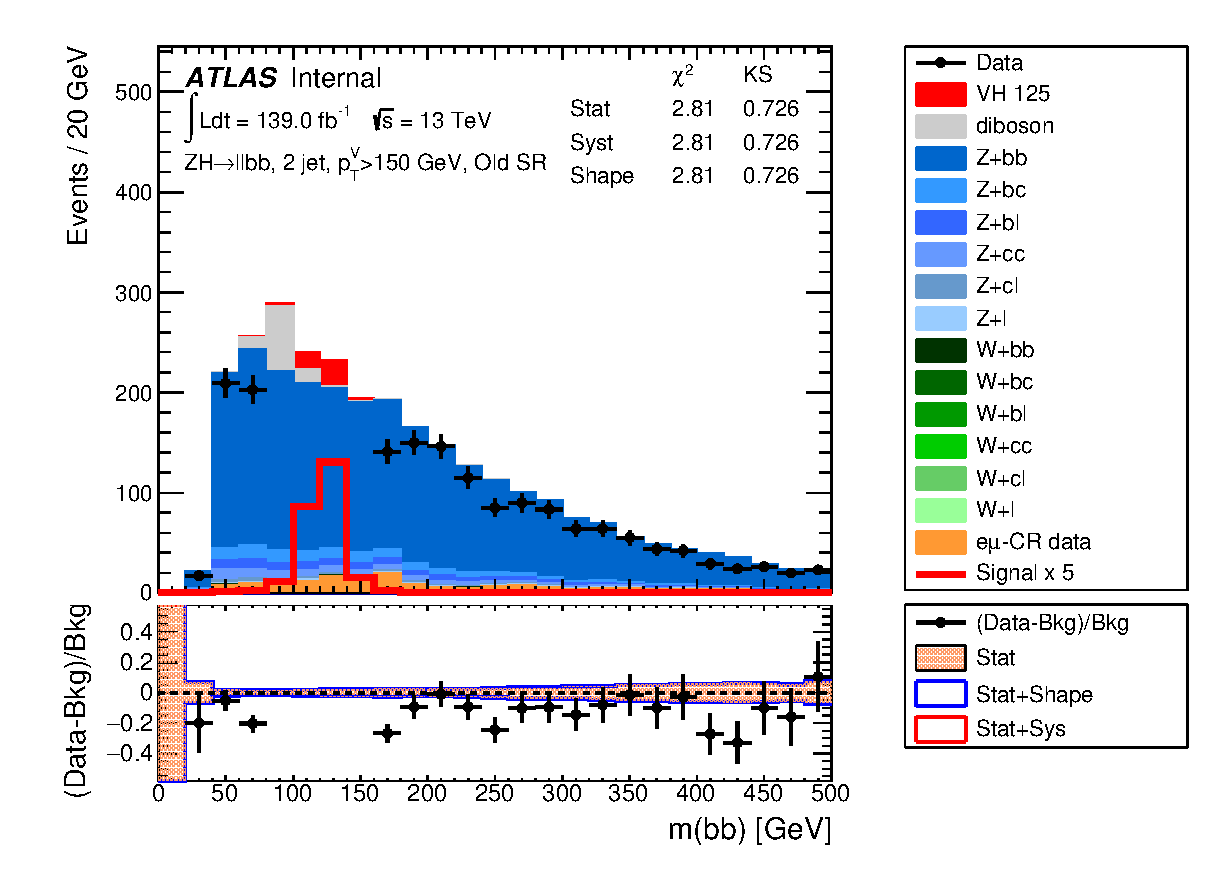
\includegraphics[width=75mm]{C_2tag2jet_150ptv_SROld_mBB.eps}
  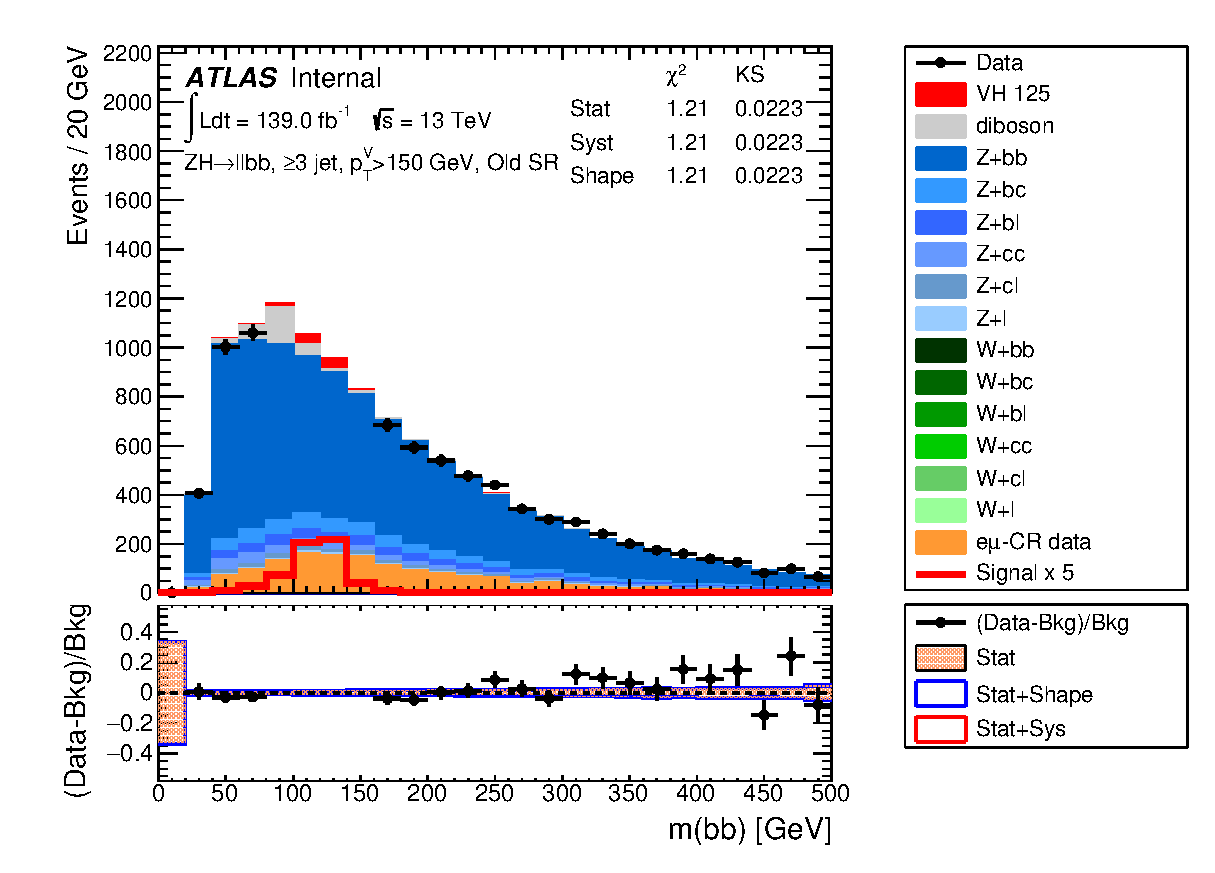
\includegraphics[width=75mm]{dataMC_ade/C_2tag3pjet_150ptv_SROld_mBB.eps}				
	\caption{Data versus prediction comparison of $m_{bb}$ distributions used to
    check how well the top $e\mu$ control region data models the shape of the
    $t\bar{t}$ and single top processes.}
	\label{fig:ttbardd-mbb}
\end{figure}
% \newcommand{\figDataMCptv}{
% \begin{figure}[bt]
% 	\begin{center}
% 		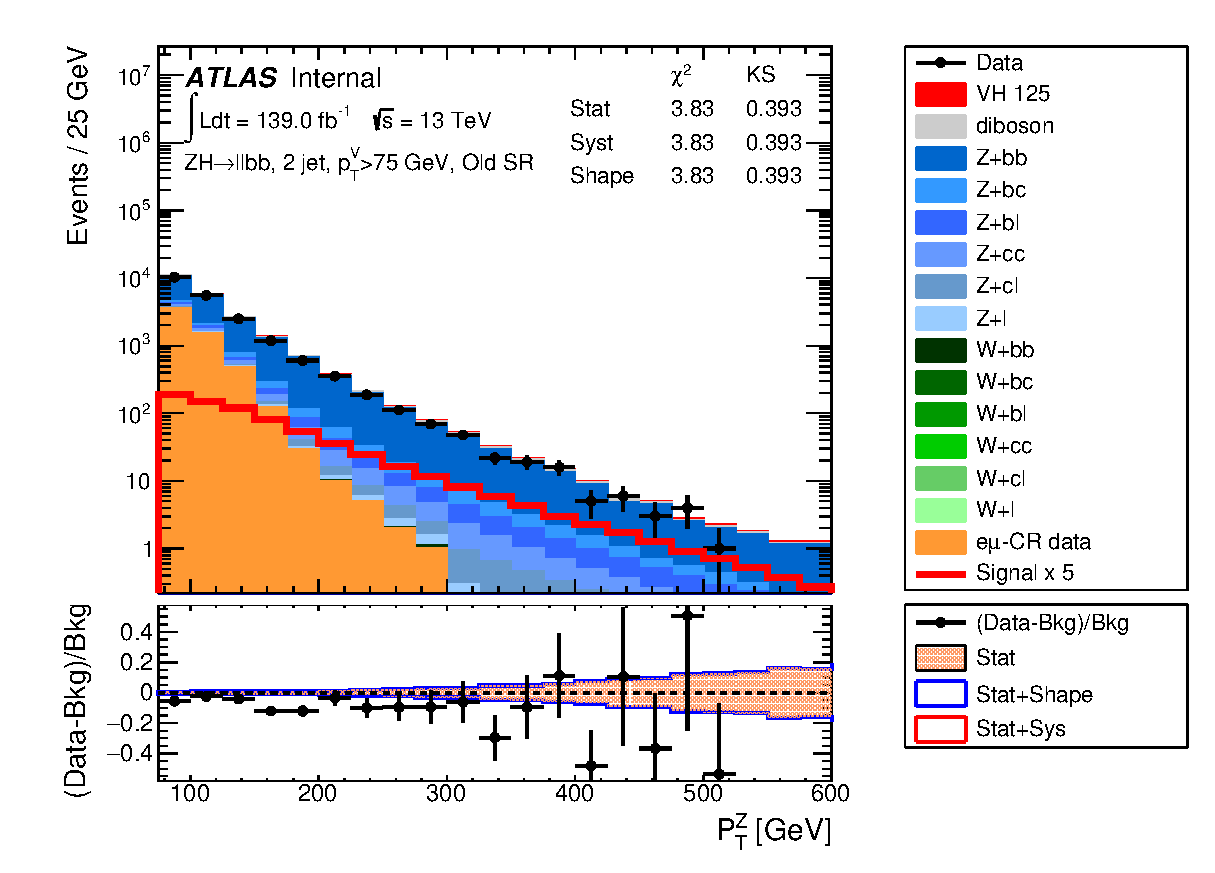
\includegraphics[width=75mm]{\ddtt@figures/dataMC_ade/C_2tag2jet_75ptv_SROld_pTV_Log.eps}
% 		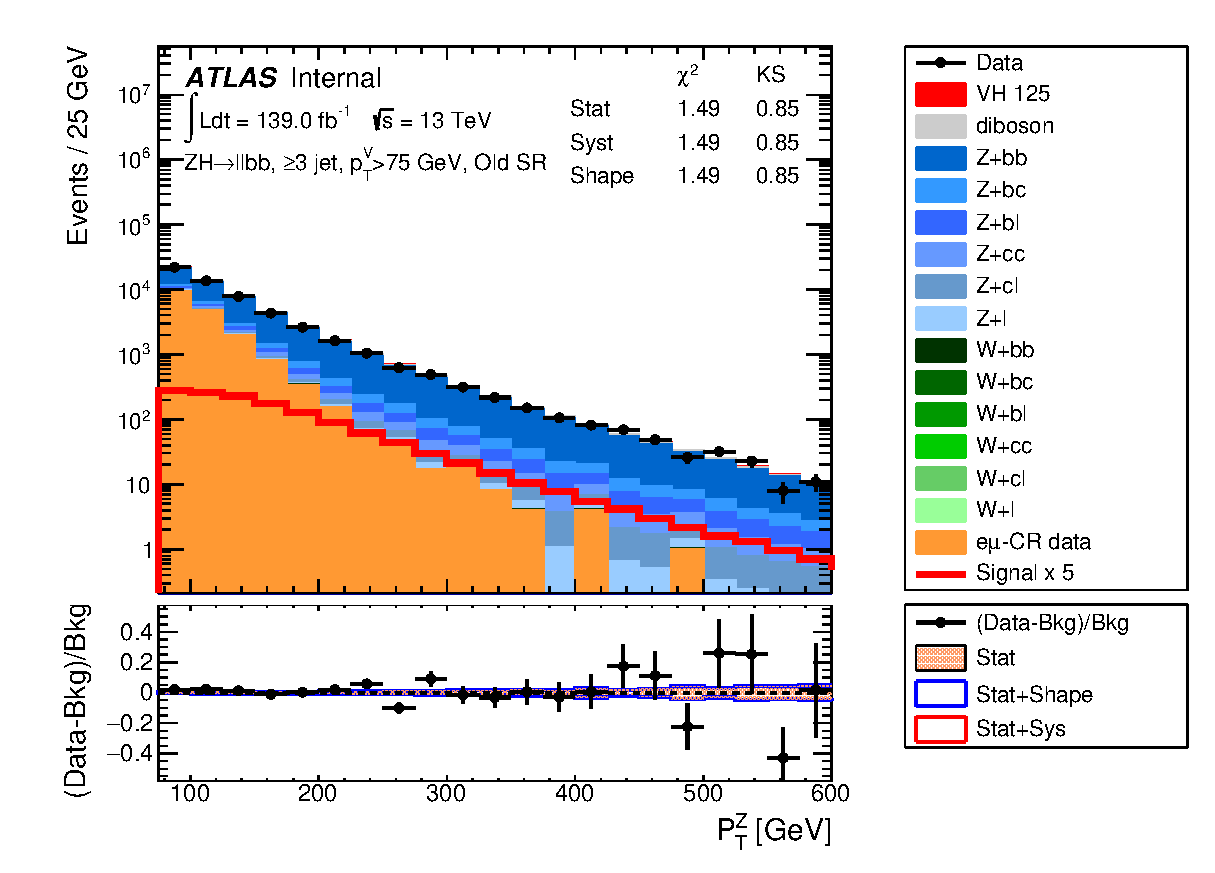
\includegraphics[width=75mm]{\ddtt@figures/dataMC_ade/C_2tag3pjet_75ptv_SROld_pTV_Log.eps}
% 	\end{center}
% 	\caption{Data-MC comparison of $p_{{\textrm T},V}$ distributions in SR in each nJet bin.}
% 	\label{fig:DataMCptv}
% \end{figure}
% }
% \newcommand{\figDataMCnjet}{
% \begin{figure}[bt]
% 	\begin{center}
% 		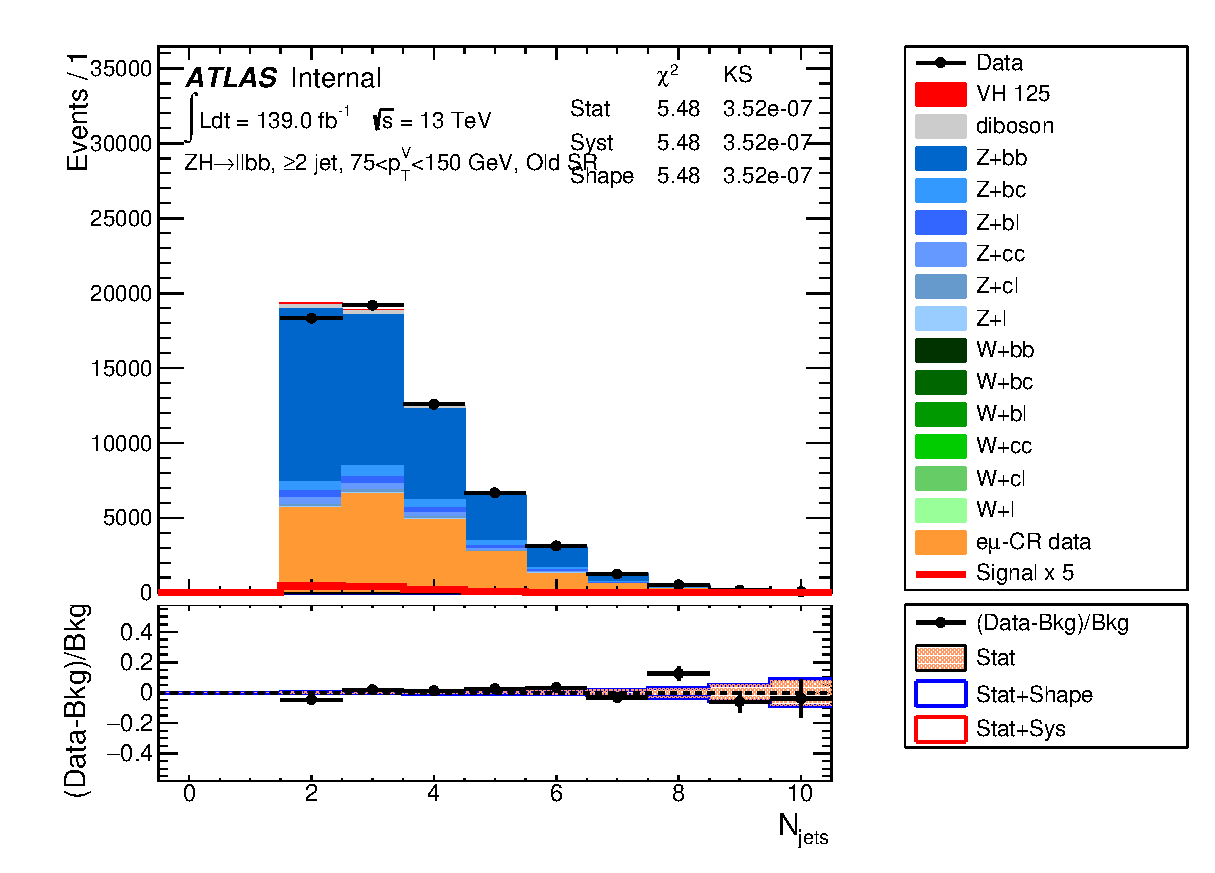
\includegraphics[width=75mm]{\ddtt@figures/dataMC_ade/C_2tag2pjet_75_150ptv_SROld_NJets.eps}
% 		\includegraphics[width=75mm]{\ddtt@figures/dataMC_ade/C_2tag2pjet_150ptv_SROld_NJets.eps}
% 	\end{center}
% 	\caption{Data-MC comparison of nJets distributions in SR in each $p_{{\textrm T},V}$ bin.}
% 	\label{fig:DataMCnjet}
% \end{figure}
% }
In order to see how the shape is modelled the scale factors controlling
normalisation of the other backgrounds have been taken from the previous
iteration of the analysis and applied, in this iteration there was no boundary
at 250~\GeV and therefore $p_T^V$ bins 75--150~\GeV and $\geq$150~\GeV are
shown. The previous iteration also did not categorise events into $\Delta R(b,
b)$ based regions and therefore the so-called SROld is shown which is the sum of
all the $\Delta R(b, b)$ regions in this version of the analysis. It can be seen
in the ratio panels that the data and prediction agree well and therefore the
prediction from the top $e\mu$ control region are considered to be accurate.

\clearpage
\newpage

\section{Systematic Uncertainties on Sub-Dominant Backgrounds}

This section details the systematic uncertainties on sub-dominant backgrounds.
None of these background processes dominate in any region of any channel of the
analysis and so they are not considered to have as large of an impact on the
analysis as the rest of the backgrounds. These descriptions will be briefer than
for the other backgrounds. All of the uncertainties of sub-dominant backgrounds
are summarised in table~\ref{tab:small_bkg_systematics}.
\begin{table}
  \resizebox{\textwidth}{!}{
    \begin{tabular}{lllll}
      \toprule
      {\bfseries Nuisance Parameter} & {\bfseries Description} & {\bfseries Categories} & {\bfseries Value} & {\bfseries Effect}  \\
      \midrule
      {\bfseries Multi-jet}&&&\\
      \texttt{SysMJNorm\_2J\_El}    & multi-jet normalization 	&  1--lepton channel, 2-jet, $e$ 	& +200\% - 100\% 	&Normalization\\
      \texttt{SysMJNorm\_3J\_El}    & multi-jet normalization 	&  1--lepton channel, 3-jet, $e$ 	& +100\% - 100\% 	&Normalization\\
      \texttt{SysMJNorm\_2J\_Mu}    & multi-jet normalization 	&  1--lepton channel, 2-jet, $\mu$       & +47\% -  29\% 	&Normalization\\
      \texttt{SysMJNorm\_3J\_Mu}    & multi-jet normalization 	&  1--lepton channel, 3-jet, $\mu$       & +100\% - 100\% 	&Normalization\\
      %% \texttt{SysMJNorm\_2J\_El}    & multi-jet normalization 	&  1--lepton channel, 2-jet, $e$, $$p_T^V$>150~\GeV$		& +200\% - 100\% 	&Normalization\\
      %% \texttt{SysMJNorm\_2J\_El\_BMin75}   & multi-jet normalization 	&  1--lepton channel, 2-jet, $e$, $$p_T^V$\in[75,150]~\GeV$		& +200\% - 100\% 	&Normalization\\
      %% \texttt{SysMJNorm\_3J\_El}    & multi-jet normalization 	&  1--lepton channel, 3-jet, $e$, $$p_T^V$>150~\GeV$		& +100\% - 100\% 	&Normalization\\
      %% \texttt{SysMJNorm\_3J\_El\_BMin75}   & multi-jet normalization 	&  1--lepton channel, 3-jet, $e$, $$p_T^V$\in[75,150]~\GeV$		& +100\% - 100\% 	&Normalization\\
      %% \texttt{SysMJNorm\_2J\_Mu}    & multi-jet normalization 	&  1--lepton channel, 2-jet, $\mu$, $$p_T^V$>150~\GeV$	        & +47\% -  29\% 	&Normalization\\
      %% \texttt{SysMJNorm\_2J\_Mu\_BMin75}   & multi-jet normalization 	&  1--lepton channel, 2-jet, $\mu$, $$p_T^V$\in[75,150]~\GeV$	& +47\% -  29\% 	&Normalization\\
      %% \texttt{SysMJNorm\_3J\_Mu}    & multi-jet normalization 	&  1--lepton channel, 3-jet, $\mu$, $$p_T^V$>150~\GeV$	        & +100\% - 100\% 	&Normalization\\
      %% \texttt{SysMJNorm\_3J\_Mu\_BMin75}  & multi-jet normalization 	&  1--lepton channel, 3-jet, $\mu$, $$p_T^V$\in[75,150]~\GeV$	& +100\% - 100\% 	&Normalization\\
      % \texttt{SysMJTrigger} & multi-jet shape & 1--lepton, electron channel & - & Shape \\
      \texttt{SysMJReduced} & multi-jet shape change with isolation criteria & 1--lepton, $e$ and $\mu$ channel & - & Shape \\
      \texttt{SysMJSFsCR} & multi-jet shape change with $W +$HF/Top scaling & 1--lepton, $e$ and $\mu$ channel & - & Shape \\
      %% \texttt{SysMJReduced} & multi-jet shape change with isolation criteria & 1--lepton, $e$ and $\mu$ channel, $$p_T^V$>150~\GeV$ & - & Shape \\
      %% \texttt{SysMJReduced\_BMin75} & multi-jet shape change with isolation criteria & 1--lepton, $e$ and $\mu$ channel, $$p_T^V$\in[75,150]~\GeV$ & - & Shape \\
      %% \texttt{SysMJSFsCR} & multi-jet shape change with $W +$HF/Top scaling & 1--lepton, $e$ and $\mu$ channel, $$p_T^V$>150~\GeV$ & - & Shape \\
      %% \texttt{SysMJSFsCR\_BMin75} & multi-jet shape change with isolation criteria & 1--lepton, $e$ and $\mu$ channel, $$p_T^V$\in[75,150]~\GeV$ & - & Shape \\
      {\bfseries Single top}&&&&\\
      \texttt{stopsNorm}    & single-top ($s$-channel) normalization 	&  all regions	& 4.6\%	&Normalization\\
      \texttt{stoptNorm}    & single-top ($t$-channel) normalization 	&  all regions	& 4.4\%	&Normalization\\
      \texttt{stopWtNorm}   & single-top ($Wt$-channel) normalization &  all regions	& 6.2\%	&Normalization\\
      \texttt{stoptAcc}     & single-top ($t$-channel) acceptance 	&  all regions & 17\% (2jets), 20\% (3jets)	&Normalization\\
      \texttt{StopWtbbAcc} 	& single-top ($Wt$ channel $Wt\rightarrow b\bar{b}$) acceptance &  all regions	& 54.9\% (2jets), 50.7\% (3jets)	&Normalization\\
      \texttt{StopWtothAcc} 	& single-top ($Wt$ channel $Wt\rightarrow oth.$) acceptance &  all regions	& 24.1\% (2jets), 21.2\% (3jets)	&Normalization\\
      \texttt{StoptPTV} & single-top ($t$-channel) $p_T^V$\ shape & all regions & - & Migration+Shape\\
      \texttt{StoptMBB} & single-top ($t$-channel) $m_{bb}$\ shape & all regions & - & Migration+Shape\\
      \texttt{StopWtPTV} & single-top ($Wt$-channel) $p_T^V$\ shape & all regions & - & Migration+Shape\\
      \texttt{StopWtMBB} & single-top ($Wt$-channel) $m_{bb}$\ shape & all regions & - & Migration+Shape\\
      {\bfseries Diboson}&&&&\\
      \texttt{SysZZNorm}    & $ZZ$ normalization 	&  all regions  & 20\%	&Normalization\\
      \texttt{SysWZNorm}    & $WZ$ normalization 	&  all regions	& 26\%	&Normalization\\
      \texttt{SysWWNorm}    & $WW$ normalization 	&  all regions	& 25\%	&Normalization\\
      \texttt{SysVZUEPSAcc} & UEPS acceptance: overall variation &  all regions & $WZ\ell\nu b\bar{b}$: 3.9\%, $ZZ\ell\ell b\bar{b}$: 5.8\%, $ZZ\nu\nu b\bar{b}$: 5.6\% & Normalization\\
      \texttt{SysVZUEPS\_J3} & UEPS acceptance: $2$- to $3$(+)-jet ratio & 3(+)jet regions & $WZ\ell\nu b\bar{b}$: 10.8\%, $ZZ\ell\ell b\bar{b}$: 3.1\%, $ZZ\nu\nu b\bar{b}$: 7.3\% & Normalization\\
      \texttt{SysWZUEPSResid\_L0} & $WZ$ UEPS acceptance: $0$-lep residual & $0$-lepton & 11.0\% & Normalization\\
      \texttt{SysZZUEPSResid\_L0} & $ZZ$ UEPS acceptance: $0$-lep residual & $0$-lepton & 6.0\% & Normalization\\
      \texttt{SysVZQCDscale\_J2} & $2$-jet QCD scale acceptance variation & 2-jet regions & $WZ\ell\nu b\bar{b}$: 12.7\%, $ZZ\ell\ell b\bar{b}$: 11.9\%, $ZZ\nu\nu b\bar{b}$: 10.3\% & Normalization\\
      \texttt{SysVZQCDscale\_J3}
            & $2$- to $3$(+) jet QCD scale acceptance ratio & 2-jet regions   & $WZ\ell\nu b\bar{b}$: -17.7\%, $ZZ\ell\ell b\bar{b}$: -16.4\%, $ZZ\nu\nu b\bar{b}$: -15.2\% & Normalization\\
                                     &  & 3(+)-jet regions & $WZ\ell\nu b\bar{b}$: 21.2\%, $ZZ\ell\ell b\bar{b}$: 10.1\%, $ZZ\nu\nu b\bar{b}$: 17.4\% & Normalization\\
      \texttt{SysVZQCDscale\_JVeto} & $4^{\text{th}}$-jet veto QCD scale acceptance variation & 3-jet, 0- and 1--lepton & $WZ \ell \nu b \bar{b}$: 19.0\%, $ZZ\nu \nu b\bar{b}$: 18.2\% & Normalization\\
      \texttt{SysggZZQCDscale} & $gg\to ZZ$ QCD scale acceptance variation & all regions & 59\% & Normalization\\
      \texttt{SysVVPTVME} & di-boson $p_T^V$\ shape & all regions & - & Migration+Shape \\ 
      \texttt{SysVVMbbME} & di-boson $m_{bb}$\ shape & all regions & - & Migration+Shape \\ 
      \texttt{SysVVPTVUEPS} & di-boson $p_T^V$\ shape variation & all regions & - & Migration+Shape \\
      \texttt{SysVVMbbUEPS} & di-boson $m_{bb}$\ shape variation & all regions & - & Migration+Shape\\
\bottomrule
\end{tabular}
}
\caption[A summary of systematic uncertainties on sub-dominant backgrounds of
the analysis.]{Small bkg syst summary}
  % Summary of the systematic
  % uncertainties for single-top, di-boson : the first column quotes the name of
  % the nuisance parameter implemented in the fit referring to a specific
  % systematic uncertainty, the second column the source of the uncertainty, the
  % third the categories and sample on which it is applied, the fourth column the
  % value of  the Gaussian prior on the NP (if applicable) and the fifth column
  % the effect of the systematic uncertainty. The listed systematic uncertainties
  % are separated in normalization effects, acceptance variations  and shape
  % systematic uncertainties.
\label{tab:small_bkg_systematics}
\end{table}
All of these systematic uncertainties are based on the comparison of different
Monte-Carlo predictions, details of the nominal predictions for multi-jet,
single top and diboson are found in tables~\ref{tab:mj-nom}, \ref{tab:st-nom},
\ref{tab:diboson-nom} respectively, with the alternative predictions found in
tables~\ref{tab:mj-alt}, \ref{tab:st-alt} and \ref{tab:diboson-alt}. (Check
multi-jet doesn't have a data-driven component).


\subsection{Multi-Jet}
Systematic uncertainties on the multi-jet background due to QCD are considered
only in the 1--lepton channel. This is due to heavy suppression of multi-jet
processes in the 0-- and 2--lepton channels. The uncertainties considered are on
the normalisation and shape effects only. For normalisation a nuisance parameter
is introduced for each category in jet multiplicity and each channel ($e$ or
$\mu$) of the multi-jet process, totalling four parameters. Two parameters
control the shape uncertainty which are associated to altering the isolation
criteria described in section~\ref{sec:lepton} and altering the scaling with
respect to the W + hf and top quark processes. 

\subsection{Single Top}
Systematic uncertainties on the single top process are applied to all regions of
the analysis and include parameters controlling the normalisation, acceptance
effects and shape effects. Normalisation is considered for the s-channel,
t-channel and Wt-channel single top decays individually. Acceptances in the
2--jet and 3--jet categories are considered for the t- and Wt-channels where the
Wt-channel has a parameter for $bb$ and Oth flavour sub-components where Oth is
defined as in~\ref{sec:ttbar-systs}. Shape uncertainties are considered for the
$p_T^V$ and $m_{bb}$ variables for the t- and Wt-channels totally four
parameters controlling the shapes.

\subsection{Diboson}
Systematic uncertainties on the diboson process are considered in all regions of
the analysis and include normalisation, acceptance and shape uncertainties.
There is one parameter controlling normalisation for each of the $WW$, $ZZ$ and
$WZ$ processes. A number of parameters controlling acceptance uncertainty due to
the underlying event and parton shower variations are introduced. There are two
for the $VZ$ process controlling the overall variation and the acceptance
between categories in jet multiplicity. There is one parameter for each of the
$WZ$ and $ZZ$ process that controls the acceptance in the 0--lepton channel.
Additionally there are four parameters controlling acceptance uncertainty
originating from the chosen QCD strength parameter, there is one for acceptance
of $VZ$ events in the 2--jet category, one to control migration of $VZ$ events
between the 2-- and 3--jet categories, one that controls acceptance changes due
to the veto based on the total number of jets in any $VZ$ event, and one that
controls the acceptance of $gg$ initiated $ZZ$ events. Four shape uncertainties
are considered, one for variations due to the matrix element calculation and one
for variations due to the underlying events and parton shower calculations, for
the $p_T^V$ and $m_{bb}$ variables.

\section{Systematic Uncertainties on the Signal Process}

Predictions of the number of events expected due to the \VHbb\ signal process
are generated as follows. Processes initiated by a $q\bar{q}$ interaction are
simulated with
\textsc{Powheg}~+~\textsc{MiNLO}~+~\textsc{Pythia}~8~\cite{Luisoni2013,
  Sjostrand2008852} at NLO whereas processes initiated by a $gg$ interaction are
simulated with \textsc{Powheg}~+~\textsc{Pythia}~8 at LO. Both sets of samples
are have the AZNLO tune~\cite{Aad:2014xaa} applied with the NNPDF3.0
PDF~\cite{Ball:2014uwa} set being used. Alternative predictions are generated 
using variations of the internal parameters of the nominal generators and also
with \textsc{Powheg}~+~\textsc{MiNLO}~+~\textsc{Herwig}~7. Details of the
nominal and alternative predictions are found in
tables~\ref{tab:VHSMsignals-nom} and~\ref{tab:VHSMsignals-alt} respectively.

The cross section that samples are normalised to is the best theoretical
prediction available which is calculated at NNLO in QCD~\cite{Brein:2003wg,
  Brein:2011vx}, NLO in EW~\cite{Denner:2012sx} and includes higher order
contributions to the gluon-induced heavy quark loop entering into the \ZH
calculation~\cite{Altenkamp:2012sx}.

A summary of the systematic uncertainties considered on the signal samples can
be found in table~\ref{tab:sig_systematics}.
\begin{table}
\resizebox{\textwidth}{!}{
\begin{tabular}{l|llcc}
\hline\hline Nuisance Parameter & Description & Categories/Sample & Value & Effect  \\
\hline
\hline
\texttt{SysTheoryBRbb}      & BR variation         & all regions   & 1.7\%                  & Normalization\\
\hline
\texttt{QCDScaleDeltaY\_qqVH}  & Scale uncertainty on qqVH production cross-section   & all reg / $qqVH$   & 0.7\%  & Normalization\\
\texttt{QCDScaleDelta75\_qqVH}  & Scale uncertainty due to $p_T^V$ STXS boundary at $75$~GeV   & all reg / $qqVH$   & -  & Migration+Shape \\
\texttt{QCDScaleDelta150\_qqVH}  & Scale uncertainty due to $p_T^V$ STXS boundary at $150$~GeV   & all reg / $qqVH$   & -  & Migration+Shape \\
\texttt{QCDScaleDelta250\_qqVH}  & Scale uncertainty due to $p_T^V$ STXS boundary at $250$~GeV   & all reg / $qqVH$   & -  & Migration+Shape \\
\texttt{QCDScaleDelta400\_qqVH}  & Scale uncertainty due to $p_T^V$ STXS boundary at $400$~GeV   & all reg / $qqVH$   & -  & Migration+Shape \\
\texttt{TheoryDelta1\_qqVH}  & Scale uncertainty due to STXS boundary at $N(jet)-N(Higgs jets)==1$   & all reg / $qqVH$   & -  & Migration+Shape \\
\texttt{TheoryDelta2\_qqVH}  & Scale uncertainty due to STXS boundary at $N(jet)-N(Higgs jets)==2$   & all reg / $qqVH$   & -  & Migration+Shape \\
\texttt{QCDScaleDeltaY\_ggZH}  & Scale uncertainty on ggZH production cross-section   & all reg / $ggZH$   & 25\%  & Normalization\\
\texttt{QCDScaleDelta75\_ggZH}  & Scale uncertainty due to $p_T^V$ STXS boundary at $75$~GeV   & all reg / $ggZH$   & -  & Migration+Shape \\
\texttt{QCDScaleDelta150\_ggZH}  & Scale uncertainty due to $p_T^V$ STXS boundary at $150$~GeV   & all reg / $ggZH$   & -  & Migration+Shape \\
\texttt{QCDScaleDelta250\_ggZH}  & Scale uncertainty due to $p_T^V$ STXS boundary at $250$~GeV   & all reg / $ggZH$   & -  & Migration+Shape \\
\texttt{QCDScaleDelta400\_ggZH}  & Scale uncertainty due to $p_T^V$ STXS boundary at $400$~GeV   & all reg / $ggZH$   & -  & Migration+Shape \\
\texttt{TheoryDelta1\_ggVH}  & Scale uncertainty due to STXS boundary at $N(jet)-N(Higgs jets)==1$   & all reg / $ggVH$   & -  & Migration+Shape \\
\texttt{TheoryDelta2\_ggVH}  & Scale uncertainty due to STXS boundary at $N(jet)-N(Higgs jets)==2$   & all reg / $ggVH$   & -  & Migration+Shape \\
\hline
\texttt{TheoryPDF\_[1-30]}  & 30 PDF4LHC uncertainties on predicted cross-section in all STXS bins   & all regions   & -  & Normalization+Shape \\
\texttt{TheoryPDFalphas}  & $\alpha_S$ variation uncertainties on predicted cross-section in all STXS bins   & all regions   & -  & Normalization+Shape \\
\hline
\texttt{TheoryPSUE\_H7}  & STXS bin acceptance uncertainty comparing \textsc{Pythia8} and \textsc{Herwig7}   & all regions   & -  & Migration+Shape \\
\texttt{TheoryPSUE\_AZNLO\_Ren}  & STXS bin acceptance uncertainty due to AZNLO renormalisation scales   & all regions   & -  & Migration+Shape \\
\texttt{TheoryPSUE\_AZNLO\_MPI}  & STXS bin acceptance uncertainty due to AZNLO MPI tune   & all regions   & -  & Migration+Shape \\
\texttt{TheoryPSUE\_AZNLO\_Var1} & STXS bin acceptance uncertainty after using Var1 AZNLO tune    & all regions   & -  & Migration+Shape \\
\texttt{TheoryPSUE\_AZNLO\_Var2} & STXS bin acceptance uncertainty after using Var2 AZNLO tune    & all regions   & -  & Migration+Shape \\
\hline
\texttt{VHNLOEWK} & $p_T^V$ shape variation from NLO EW correction & all regions & - & Migration+Shape\\
\texttt{VHUEPSMbb}  & $m_{bb}$\ shape variation from UEPS variations & all regions & - & Migration+Shape\\
\texttt{VHQCDscaleMbb} & $m_{bb}$\ shape variation from scale variations & all regions & - & Migration+Shape\\
\texttt{VHQCDscaleMbb\_ggZH} & \multicolumn{4}{l}{$\rightarrow$ Decorrelate: "\texttt{\_qqVH}" and "\texttt{\_ggZH}"} \\
\hline\hline
\end{tabular}}
\caption[Summary of $VH$ signal nuisance parameters.]{Summary of the systematic uncertainties for SM VH processes: the first column quotes the name of the nuisance parameter implemented in the fit referring to a specific systematic uncertainty, the second column the source of the uncertainty, the third the categories and sample on which it is applied, the fourth column the value of  the Gaussian prior on the NP (if applicable) and the fifth column the effect of the systematic uncertainty. The listed systematic uncertainties are separated in branching ratio uncertainty, STXS cross-section QCD scale and PDF variations, STXS acceptance effects and shape systematic uncertainties.}
{\label{tab:sig_systematics}}
\end{table}
The majority of these uncertainties account for migration between STXS bins
(which are defined in $p_T^V$) due to the QCD scale uncertainty. Parameters are
decorrelated for each STXS bin boundary (75, 150, 250, 400)~\GeV and for the
$q\bar{q}$ and $gg$ initiated processes. Similarly there are parameters that
control for migration at the relevant $N_{\text{jet}} - N_{H\text{jet}}$
boundaries that are decorrelated in the same way. Additionally there are
parameters that control the uncertainty of the overall cross-section of the
$q\bar{q}$ and $gg$ processes due to the QCD scale uncertainty. More parameters
control uncertainties arising from the choice of PDF set which control both
shape and normalisation. A single parameter controls for the uncertainty of the
branching ratio of the $H \to b{\bar{b}}$ decay. Finally several parameters
control  $p_T^V$ and $m_{bb}$ shape variations due to NLO EW corrections and
underlying event and parton shower calculations, with the latter also being
decorrelated based on sub-process. 